\documentclass{report}
\usepackage{spikey}
\usepackage{amsmath}
\usepackage{mathrsfs}
\usepackage{amssymb}
\usepackage{soul}
\usepackage{float}
\usepackage{graphicx}
\usepackage{hyperref}
\usepackage{fancyhdr}
\usepackage{xcolor}
\usepackage{chngcntr}
\usepackage{centernot}
\usepackage[shortlabels]{enumitem}
\usepackage[margin=1truein]{geometry}
\usepackage{tkz-graph}
\usepackage{dsfont}
\usepackage{caption}
\usepackage{subcaption}

\usepackage{setspace}
\linespread{1.15}
\usepackage[margin=1truein]{geometry}

\counterwithin{equation}{section}
\counterwithin{figure}{section}

\pagestyle{fancy}
\lhead{MAT395: Independent Reading in Mathematics}

\usepackage[
    type={CC},
    modifier={by-nc},
    version={4.0},
]{doclicense}

\title{MAT395 Independent Reading in Mathematical Economics\\ \small Individual Decision Making, Partial Equilibrium, General Equilibrium, and Fundamental Theorems of Welfare Economics}
\date{\today}
\author{Tianyu Du}
\begin{document}
	\maketitle
	\doclicenseThis
	\begin{itemize}
		\item GitHub: \url{https://github.com/TianyuDu/Spikey_UofT_Notes}
		\item Website: \url{TianyuDu.com/notes}
	\end{itemize}
	\tableofcontents
	
	\chapter{Individual Choices}
	\section{Chapter 1. Preference and Choice}
	\subsection{Preference Relations}
	
		\begin{definition} \quad
			\begin{enumerate}[(i)]
				\item The \textbf{strict preference} relation, $\succ$, is defined by
					\begin{equation}
						x \succ y \iff x \pref y \land \neg (y \pref x)
					\end{equation}
				\item The \textbf{indifference} relation, $\sim$, is defined by
					\begin{equation}
						x \sim y \iff x \pref y \land y \pref x
					\end{equation}
			\end{enumerate}
		\end{definition}
	
		\begin{definition}[1.B.1]
			The preference relation $\pref$ is \textbf{rational} if it possesses the following two properties
			\begin{enumerate}[(i)]
				\item \emph{Completeness} 
					\begin{equation}
						\forall x, y \in X,\ x \pref y \lor y \pref x
					\end{equation}
				\item \emph{Transitivity}
					\begin{equation}
						\forall x, y, z \in X,\ x \pref y \land y \pref z \implies x \pref z
					\end{equation}
			\end{enumerate}
		\end{definition}
	
		\begin{proposition}[1.B.1]
			If $\pref$ is rational, then
			\begin{enumerate}[(i)]
				\item $\succ$ is both \textbf{reflexive} ($\neg\ x \succ x$) and \textbf{transitive} ($x \succ y \land y \succ z \implies x \succ z$);
				\item $\sim$ is both \textbf{reflexive} and \textbf{transitive};
				\item $x \succ y \pref z \implies x \succ z$.
			\end{enumerate}
		\end{proposition}
		
		\begin{example}
			Typical scenarios when transitivity of preference is violated:
			\begin{enumerate}[(i)]
				\item \emph{Just perceptible differences};
				\item \emph{Framing problem};
				\item \emph{Observed preference might from the result of the interaction of several more primitive rational preferences (Condorcet paradox)};
				\item \emph{Change of tastes}.
			\end{enumerate}
		\end{example}
		
		\begin{definition}[1.B.2]
			A function $u: X \to \R$ is a \textbf{utility function representing preference relation} $\pref$ if
			\begin{equation}
				\forall x, y \in X,\ x \pref y \iff u(x) \geq u(y)
			\end{equation}
		\end{definition}
		
		\begin{proposition}[1.B.2]
			If a preference relation $\pref$ can be represented by a utility function, then $\pref$ is rational.
		\end{proposition}
	
	\subsection{Choice Rules}
		\begin{definition}
			A \textbf{choice structure}, $(\mathscr{B}, C(\cdot))$, is a tuple consists of
			\begin{enumerate}[(i)]
				\item The collection of \textbf{budget sets} $\mathscr{B}$, which is a set of nonempty subsets of $X$.
				\item The \textbf{choice rule}, $C(B) \subset B$, is a \emph{correspondence} for every $B \subset \mathscr{B}$ denotes the individual's choice from among the alternatives in $B$. If $C(B)$ is not a singleton, it can be interpreted as the \emph{acceptable alternatives} in $B$, which the individual would actually chosen if the decision-making process is run repeatedly. 
			\end{enumerate}
		\end{definition}
		
		\begin{definition}[1.C.1]
			The choice structure $(\mathscr{B}, C(\cdot))$ satisfies the \textbf{weak axiom of revealed preference} if
			\begin{equation}
				\Big(\underbrace{
					\exists B \in \mathscr{B}\ s.t.\ x, y \in B \land x \in C(B)
					}_{\tx{$x \pref* y$ revealed.}}
				\Big)
				\implies 
				\Big(
					\forall B' \in \mathscr{B}\ s.t.\ x, y \in B',\ y \in C(B') \implies x \in C(B')
				\Big)
			\end{equation}
		\end{definition}
		
		\begin{definition}
			Given a choice structure $(\mathscr{B}, C(\cdot))$, the \textbf{revealed preference relation} $\pref^*$ is defined as
			\begin{equation}
				x \pref^* y \iff \exists B \in \mathscr{B}\ s.t.\ x, y \in B \land x \in C(B)
			\end{equation}
		\end{definition}
		
		\begin{remark}[Interpretation on the definition of WARP]
			If $x$ is \emph{revealed} at least as good as $y$, then $y$ cannot be revealed preferred to $x$.
		\end{remark}
	
	\subsection{The Relationship between Preference Relations and Choice Rules}
		\begin{definition}
			Given \ul{rational} preference relation $\pref$ on $X$, the \textbf{preference-maximizing choice rule} is defined as 
			\begin{equation}
				C^*(B, \pref) := \{x \in B: x \pref y\ \forall y \in B\}\ \forall B \in \mathscr{B}
			\end{equation}
			We say the \ul{rational} preference relation \textbf{generates} the choice structure $(\mathscr{B}, C^*(\cdot, \pref))$.
		\end{definition}
		
		\begin{assumption}
			Assume $C^*(B, \pref) \neq \varnothing$ for all $B \in \mathscr{B}$.
		\end{assumption}
		
		\begin{proposition}[1.D.1 (\hl{Rational $\to$ WARP})]
			Suppose that $\pref$ is a \ul{rational} preference relation. Then the choice structure generated by $\pref$, $(\mathscr{B}, C^*(\cdot, \pref))$, satisfies the weak axiom.
		\end{proposition}
		
		\begin{definition}[1.D.1]
			Given choice structure $(\mathscr{B}, C(\cdot))$, we say that the \ul{rational preference relation $\pref$ \textbf{rationalizes} $C(\cdot)$ relative to $\mathscr{B}$} if
			\begin{equation}
				C(B) = C^*(B, \pref)\ \forall B \in \mathscr{B}
			\end{equation}
			That is, \emph{$\pref$ generates the choice structure $(\mathscr{B}, C(\cdot))$}.
		\end{definition}
		
		\begin{remark}
			In general, for a given choice structure $(\mathscr{B}, C(\cdot))$, there may be more than one rational preference relation $\pref$ rationalizing it.
		\end{remark}
		
		\begin{proposition}[1.D.2 (\hl{WARP $\to$ Rational})]
			If $(\mathscr{B}, C(\cdot))$ is a choice structure such that
			\begin{enumerate}[(i)]
				\item The weak axiom is satisfied;
				\item $\mathscr{B}$ includes all subsets of $X$ up to three elements.
			\end{enumerate}
			Then there is a rational preference relation $\pref$ that rationalizes $C(\cdot)$ relative to $\mathscr{B}$.
		\end{proposition}
	
	\section{Chapter 2. Consumer Choice}
		\subsection{Commodities}
			\begin{definition}
				Assume the number of \textbf{commodities} is finite and equal to $L$. In general, a \textbf{commodity vector} or \textbf{commodity bundle} is an element in a \textbf{commodity space}, typically $\R^L$.
				\begin{equation}
					\vex := \begin{bmatrix}
						x_1 \\ \vdots \\ x_L
					\end{bmatrix} \in \R^L
				\end{equation}
 			\end{definition}
 			
 			\begin{remark}[Time Aggregation]
 				The time/location of commodity matters in some scenarios, and can be built into the definition of a commodity.
 			\end{remark}
 			
 			\begin{remark}
 				We should also note that in some contexts it becomes convenient, and even necessary, to expand the set of commodities to include goods and services that may potentially be available for purchase but are not actually so and even some that may be available by means other than market exchange.
 			\end{remark}
 		
 		\subsection{The Consumption Set}
 			\begin{definition}
 				The \textbf{consumption set} is a subset of the commodity space $\R^L$, denoted by $X \subset \R^L$, whose elements are the consumption bundles that the individual can conceivably consume given the physical constraints imposed by his environment.
 			\end{definition}
 			
 			\begin{assumption}
 				For simplicity, we assume the consumption set to be $\R_+^L$, which is \emph{convex}.
 				\begin{equation}
 					X := \R_+^L = \{\vex \in \R^L: x_{\ell} \geq 0,\ \forall \ell \in [L]\}
 				\end{equation}
 			\end{assumption}
 			
 		\subsection{Competitive Budgets}
 			\begin{definition}
 				A \textbf{price vector} is defined as
 				\begin{equation}
 					\vep := \begin{bmatrix} p_1 \\ \vdots \\ p_L \end{bmatrix} \in \R^L
 				\end{equation}
 				For simplicity, here we always assume 
 				\begin{enumerate}[(i)]
 					\item \emph{Positive price}: $\vep \gg \ve{0}$;
 					\item \emph{Price-taking assumption}: $\vep$ is beyond the influence of the consumer.
 				\end{enumerate}
 			\end{definition}
 			
 			\begin{definition}[2.D.1]
 				The \textbf{Walrasian}, or \textbf{competitive budget set} is defined as
 				\begin{equation}
 					B_{\vep, w} := \{
 						\vex \in \R^L_+: \vep \cdot \vex \leq w
 					\}
 				\end{equation}
 				where $w$ is the \emph{wealth} of consumer, and assumed to be positive.
 			\end{definition}
 			
 			\begin{definition}
 				The \textbf{consumer's problem} is choosing a consumption bundle $\vex \in B_{\vep, w}$, for each given $(\vep, w) \in \R^L_{++}$.
 			\end{definition}
 			
 			\begin{definition}
 				The set $\{\vex \in \R^L_+: \vep \cdot \vex = w\}$ is called the \textbf{budget hyperplane}.
 			\end{definition}
 			
 			\begin{proposition}
 				The price vector $\vep$ is orthogonal to the budget hyperplane.
 			\end{proposition}
 			
 			\begin{proposition}
 				The Walrasian budget set $B_{\vep, w}$ is a \emph{convex} set.
 			\end{proposition}
 		
 		\subsection{Demand Functions and Comparative Statics}
 			\begin{definition}
 				The consumer's \textbf{Walrasian demand correspondence} $x(\vep, w): \R_{++}^{L+1} \rightrightarrows \R_+^L$ assigns a \emph{set} of chosen consumption bundles for each price-wealth pair $(\vep, w)$. When $x(\vep, w)$ is single-valued, we refer to it as a \textbf{demand function}
 				\begin{equation}
 					\vex(\vep, w) = 
 					\begin{bmatrix}
 						x_1(\vep, w) \\
 						x_2(\vep, w) \\
 						\vdots \\
 						x_L(\vep, w)
 					\end{bmatrix}
 				\end{equation}
 			\end{definition}
 			
 			\begin{definition}[2.E.1]
 				The Walrasian demand correspondence $x(\vep, w): \R_{++}^{L+1} \rightrightarrows \R_+^L$ is \textbf{homogenous of degree zero} if 
 				\begin{equation}
 					x(\alpha \vep, \alpha w) = x(\vep, w)\ \forall (\vep, w, \alpha) \in \R_{++}^{L+2}
 				\end{equation}
 				Also note that
 				\begin{equation}
 					B_{\vep, w} = B_{\alpha \vep, \alpha w}\ \forall (\vep, w, \alpha) \in \R_{++}^{L+2}
 				\end{equation}
 			\end{definition}
 			
 			\begin{definition}[2.E.2]
 				The Walrasian demand correspondence $x(\vep, w)$ satisfies \textbf{Walras' law} if
 				\begin{equation}
 					\forall (\vep, w) \gg \ve{0},\ \forall \vex \in x(\vep, w),\ \vep \cdot \vex = w
 				\end{equation}
 			\end{definition}
 			
 			\begin{assumption}
 				For simplicity, we assume $x(\vep, w)$ is always \emph{single-valued, continuous and differentiable}.
 			\end{assumption}
 			
 			\begin{proposition}
 				The \textbf{family of Walrasian budget sets} defined as
 				\begin{equation}
 					\mathscr{B}^{\mathscr{W}} := \{B_{\vep, w}: {\vep, w} \gg \ve{0}\}
 				\end{equation}
 				altogether with Walrasian demand homogeneous to degree zero forms a \emph{choice structure}
 				\begin{equation}
 					(\mathscr{B}^{\mathscr{W}}, x(\cdot))
 				\end{equation} 
 			\end{proposition}
 		
 			\begin{definition}
 				For fixed prices $\overline{\vep} \in \R_{++}^L$, the function of wealth $\vex(\overline{\vep}, w)$ is called consumer's \textbf{Engel function}. Its image in $\R^L_+$,
 				\begin{equation}
 					E_{\overline{\vep}} := \{\vex(\overline{\vep}, w): w \in \R_{++}\} \subset \R^L_+
 				\end{equation}
 				is defined as the \textbf{wealth expansion path}.
 			\end{definition}
 			
 			\begin{definition}
 				Given $(\vep, w)$, the \textbf{wealth effect} is defined as
 				\begin{equation}
 					D_w \vex(\vep, w) 
 					= \begin{bmatrix}
 						\pd{x_1(\vep, w)}{w} \\
 						\pd{x_2(\vep, w)}{w} \\
 						\vdots \\
 						\pd{x_L(\vep, w)}{w}
 					\end{bmatrix} \in \R^L
 				\end{equation}
 				For the $\ell$-th commodity, it's called \textbf{normal} at $(\vep, w)$ if $\pd{x_{\ell}(\vep, w)}{w} \geq 0$, and \textbf{inferior} otherwise. And the $\ell$-th commodity is normal/inferior if its normal/inferior every where in $\R_{++}^{L+1}$. 
 			\end{definition}
 			
 			\begin{definition}
 				The \textbf{offer curve} is defined as the locus
 				\begin{equation}
 					\{\vex(\vep, w): p_j > 0\}
 				\end{equation}
 				for any chosen $j$.
 			\end{definition}
 			
 			\begin{definition}
 				Good $\ell$ is said to be a \textbf{Giffen good} at $(\vep, w)$ if
 				\begin{equation}
 					\pd{x_\ell(\vep, w)}{p_\ell} > 0
 				\end{equation}
 			\end{definition}
 			
 			\begin{definition}
 				The \textbf{price effects} at $(\vep, w)$ is defined as
 				\begin{equation}
 					D_{\vep} (\vep, w) = 
 					\begin{bmatrix}
 						\pd{x_1(\vep, w)}{p_1} & \cdots & \pd{x_1(\vep, w)}{p_L} \\
 						& \ddots & \\
 						\pd{x_L(\vep, w)}{p_1} & \cdots & \pd{x_L(\vep, w)}{p_L}
 					\end{bmatrix}
 				\end{equation}
 			\end{definition}
 			
 			\begin{proposition}[2.E.1]
 				If the Walrasian demand function $x(\vep, w)$ is homogenous of degree zero, then for all $\vep$ and $w$, then
 				\begin{equation}
 					\sum_{k=1}^{L} \frac{\partial x_{\ell}(\vep, w)}{\partial p_{k}} p_{k}+\frac{\partial x_{\ell}(\vep, w)}{\partial w} w=0 \text { for } \ell=1, \ldots, L
 				\end{equation}
 				Equivalently,
 				\begin{equation}
 					D_{\vep} \vex (\vep, w)\ \vep + D_w \vex(\vep, w)\ w = \ve{0}
 				\end{equation}
 				\begin{proof}
 					Apply \emph{Euler's theorem} on homogenous functions to each component $x_\ell$.
 					\begin{gather}
 						\underbrace{D_{(\vep, w)} \vex(\vep, w)}_{L \times (L+1)} \cdot \underbrace{(\vep, w)}_{(L+1) \times 1} = 0\ \vex(\vep, w) = \ve{0} \\
 						\implies [\underbrace{D_{\vep} (\vep, w)}_{L \times L} | \underbrace{D_w \vex(\vep, w)}_{L \times 1}] \cdot (\vep, w) = D_{\vep} (\vep, w)\ \vep + D_w \vex(\vep, w)\ w = \ve{0}
 					\end{gather}
 				\end{proof}
 			\end{proposition}
 			
 			\begin{definition}
 				The \textbf{elasticities of demand $\ell$ with respect to price $k$ and wealth} is defined as 
 				\begin{gather}
 					\varepsilon_{\ell, k} (\vep, w) := \pd{x_\ell (\vep, w)}{p_k} \frac{p_l}{x_\ell (\vep, w)}\\
 					\varepsilon_{\ell, w} (\vep, w) := \pd{x_\ell (\vep, w)}{w} \frac{w}{x_\ell (\vep, w)}
 				\end{gather}
 			\end{definition}
 			
  			\begin{corollary}
  				Dividing both sides of the equality in proposition (2.E.1) by $x_{\ell}$ gives
 				\begin{equation}
 					\sum_{k=1}^L \varepsilon_{\ell, k}(\vep, w) + \varepsilon_{\ell, w}(\vep, w) = 0\ \forall \ell \in \{1, \ldots, L\}
 				\end{equation}
 			\end{corollary}
 			
 			\begin{proposition}[2.E.2 Cournot Aggregation]
 				If the Walrasian demand function $x(\vep, w)$ satisfies \emph{Walras' law}, then for every $(\vep, w)$,
 				\begin{equation}
 					\sum_{\ell=1}^{L} p_{\ell} \frac{\partial x_{\ell}(\vep, w)}{\partial p_{k}}+x_{k}(\vep, w)= 0 \quad \text { for } k=1, \ldots, L
 				\end{equation}
 				Equivalently,
 				\begin{equation}
 					\vep^T D_{\vep} \vex (\vep, w) + \vex(\vep, w)^T = \ve{0}^T
 				\end{equation}
 				\begin{proof}
 					Differentiate both sides of Walras' law identity $\vep^T \vex = w$ with respect to $\vep$.
 				\end{proof}
 			\end{proposition}
 			
 			\begin{proposition}[2.E.3. Engel Aggregation]
 				If the Walrasian demand function $x(\vep, w)$ satisfies \emph{Walras' law}, then for every $(\vep, w)$,
 				\begin{equation}
 					\sum_{\ell=1}^{L} p_{\ell} \frac{\partial x_{\ell}(\vep, w)}{\partial w}=1
 				\end{equation}
 				or equivalently
 				\begin{equation}
 					\vep \cdot D_{w} x(\vep, w) = 1
 				\end{equation}
 				\begin{proof}
 					Differentiate both sides of Walras' law identity $\vep^T \vex = w$ with respect to $w$.
 				\end{proof}
 			\end{proposition}
 		
 			\begin{proposition}[Exer. 2.E.2]
 				\begin{gather}
 					\sum_{\ell=1}^{L} b_{\ell}(\vep, w) \varepsilon_{\ell k}(\vep, w)+b_{k}(\vep, w)=0
 				\end{gather}
 				and
 				\begin{gather}
 					\sum_{\ell=1}^{L} b_{\ell}(\vep, w) \varepsilon_{\ell w}(\vep, w)=1
 				\end{gather}
 				where $b_\ell := \frac{x_\ell p_\ell}{w}$ is defined to be the portion of wealth spent on commodity $\ell$.
 			\end{proposition}
 			
 		\subsection{The Weak Axiom of Revealed Preference and the Law of Demand}
 			\begin{assumption}
 				In the section, we assume $\vex(\vep, w)$ is 
 				\begin{enumerate}[(i)]
 					\item Single-valued;
 					\item homogeneous to degree zero;
 					\item satisfies Walras' law.
 				\end{enumerate}
 			\end{assumption}
 			
 			\begin{definition}[2.F.1]
 				The Walrasian demand function $\vex(\vep, w)$ satisfies the \textbf{weak axiom of revealed preference} if for every two $(\vep, w), (\vep', w') \in \R_{++}^{L+1}$,
 				\begin{gather}
 					\underbrace{\vep \cdot \vex(\vep', w') \leq w
 					\land \vex(\vep, w) \neq \vex(\vep', w')}_{\tx{revealed: } \vex(\vep, w) \succ^* \vex(\vep', w')}
 					\implies \vep' \cdot \vex(\vep, w) > w'
 				\end{gather}
 				Equivalently,
 				\begin{equation}
 					\vex(\vep', w') \in B_{\vep, w} \land \vex(\vep', w') \centernot \in C(B_{\vep, w}) \implies \vex(\vep, w) \centernot \in C(B_{\vep', w'})
 				\end{equation}
 			\end{definition}
 			
 			\begin{corollary}[Equivalent Definition ]
 				The weak axiom says, given our assumptions and $\vex(\vep_1, w_1) \neq \vex(\vep_2, w_2)$, we \ul{cannot} have both 
 				\begin{equation}
 					\vex(\vep_1, w_1) \in B_{\vep_2, w_2} \land \vex(\vep_2, w_2) \in B_{\vep_1, w_1}
 				\end{equation}
 			\end{corollary}
 			
 			\begin{definition}
 				A price change $\Delta \vep$ is a \textbf{Slutsky compensated price change} if the consumer is given a \textbf{Slutsky wealth compensation} with amount
 				\begin{equation}
 					\Delta w = \Delta \vep \cdot \vex(\vep, w)
 				\end{equation}
 				such that the consumer's initial consumption is just affordable at the new price.
 			\end{definition}
 			
 			\begin{proposition}[2.F.1]
 				Suppose that the Walrasian demand function $\vex(\vep', w')$ is homogenous of degree zero and satisfies Walras' law. Then $\vex(\vep', w')$ satisfies the weak axiom \ul{if and only if} the following property holds: \\
 				For any \emph{compensated price change} from $(\vep, w)$ to $(\vep', w' := \vep' \cdot \vex(\vep, w))$,
 				\begin{equation}
 					\Delta \vep \cdot \Delta \vex \leq 0
 				\end{equation}
 				with strict inequality whenever $\vex(\vep, w) \neq \vex(\vep', w')$.
 			\end{proposition}
 			
 			\begin{corollary}[Compensated Law of Demand]
 				$\Delta \vep \cdot \Delta \vex \leq 0$ says demand and price move in opposite directions, \emph{under Slutsky compensation}.
 			\end{corollary}
 			
 			\begin{definition}
 				At infinitesimal price change, the Slutsky compensation can be written as 
 				\begin{equation}
 					dw = \vex(\vep, w) \cdot d\vep
 				\end{equation}
 				and the compensated law of demand becomes
 				\begin{equation}
 					d\vep \cdot d\vex \leq 0
 				\end{equation}
 				Then the total derivative of $\vex$ is 
 				\begin{align}
 					d\vex &= D_\vep\vex(\vep, w)\ d\vep + D_w \vex(\vep, w)\ dw \\
 					&= D_\vep\vex(\vep, w)\ d\vep + D_w \vex (\vep, w)\ [\vex(\vep, w) \cdot d\vep] \\
 					&= [\underbrace{D_\vep\vex(\vep, w)}_{L \times L} + \underbrace{D_w \vex (\vep, w)}_{L \times 1} \underbrace{\vex(\vep, w)^T}_{1 \times L}] d\vep \\
 					&\implies d\vep^T 
 					\underbrace{[D_\vep\vex(\vep, w) + D_w \vex (\vep, w) \vex(\vep, w)^T]}_{L \times L} d\vep \leq 0
 				\end{align}
 				and the \textbf{Slutsky/substitution matrix} is defined as
 				\begin{gather}
 					S(\vep, w) := [D_\vep\vex(\vep, w) + D_w \vex (\vep, w) \vex(\vep, w)^T] \\
 					s_{\ell k} = \underbrace{\pd{x_\ell(\vep, w)}{p_k}}_{\tx{total effect}} + \underbrace{\pd{x_\ell(\vep, w)}{w} x_k (p, w)}_{\tx{wealth effect}}
 				\end{gather}
 				where $s_{\ell k}$ is the \textbf{substitution effect}.
 			\end{definition}
 			
 			\begin{remark}
 				The above identity (Slutsky equation) suggests the total impact of price change in $p_k$ on demand for $x_{\ell}$ can be decomposed into two portions, substitution effect and income effect.
 			\end{remark}
 			
  			\begin{corollary}[Slutsky Equation]
 				\begin{equation}
 					\frac{\partial x_{i}(\mathbf{p}, w)}{\partial p_{j}}=\frac{\partial h_{i}(\mathbf{p}, u)}{\partial p_{j}}-\frac{\partial x_{i}(\mathbf{p}, w)}{\partial w} x_{j}(\mathbf{p}, w)
 				\end{equation}
 			\end{corollary}
 			
 			\begin{remark}
 				Consider the scenario when only $p_k$ changes, with Slutsky compensation, consumer's wealth changes by $dw = x_k(\vep, w) dp_k$. So the wealth effect on $x_\ell$ is $\pd{x_\ell}{w} dw = \pd{x_\ell}{w} x_k(\vep, w) dp_k$.
 			\end{remark}
 			
 			\begin{proposition}[2.F.2]
 				If a differentiable Walrasian demand function $\vex(\vep, w)$ satisfies Walras' law, homogeneity of degree zero, and the weak axiom, then at any $(\vep, w)$, the Slutsky matrix $S(\vep, w)$ is negative semi-definite.
 			\end{proposition}
 			
 			\begin{corollary}
 				Given $S(\vep, w)$ is negative semi-definite, we have
 				\begin{align}
 					\ve{e}_{\ell}^T S(\vep, w) \ve{e}_{\ell} \leq 0\ \forall \ell \in \{1, \ldots, L\} \\
 					\implies s_{\ell \ell} \leq 0\ \forall \ell \in \{1, \ldots, L\}
 				\end{align}
 				which suggests the \emph{substitution effect of good $\ell$ with respect to its own price is always negative}.
 			\end{corollary}
 			
 			\begin{remark}
 				Proposition 2.F.2 does \emph{not} imply, in general, that the matrix $S(\vep, w)$ is symmetric.
 			\end{remark}
 			
 			\begin{proposition}[2.F.3]
 				Suppose that the Walrasian demand function $\vex(\vep, w)$ is differentiable, homogenous of degree zero, and satisfies Walras' law. Then for every $(\vep, w)$
 				\begin{equation}
 					\vep^T S(\vep, w) = \ve{0} \land S(\vep, w) \vep = \ve{0}
 				\end{equation}
 				\begin{proof}
 					By propositions 2.E.1 to 2.E.3.
 				\end{proof}
 			\end{proposition}
 	
 	\section{Chapter 3. Classical Demand Theory}
 		\subsection{Preference Relations: Basic Properties}
 			\begin{definition}[3.B.1]
 				The preference relation $\pref$ on $X$ is \textbf{rational} if it possesses the following two properties
 				\begin{enumerate}[(i)]
 					\item \emph{Completeness.} $\forall \vex, \vey \in X,\ \vex \pref \vey \lor \vey \pref \vex$;
 					\item \emph{Transitivity.} $\forall \vex, \vey, \vez \in X,\ \vex \pref \vey \land \vey \pref \vez \implies \vex \pref \vez$.
 				\end{enumerate}
 			\end{definition}
 			
 			\subsubsection{Desirability Assumptions}
 			
 			\begin{definition}[3.B.2]
 				The preference relation $\pref$ on $X$ is \textbf{monotone} if $\vex \in X$ and $\vey \gg \vex \implies \vey \succ \vex$; It is \textbf{strongly monotone} if $\vey \geq \vex \land \vex \neq \vey \implies \vey \succ \vex$.
 			\end{definition}
 			
 			\begin{remark}
 				If $\pref$ is monotone, we may have indifference with respect to an increase in the amount of some but not all commodities.
 			\end{remark}
 			
 			\begin{definition}[3.B.3]
 				A preference relation $\pref$ on $X$ is \textbf{locally nonsatiated} if
 				\begin{equation}
 					\forall \vex \in X, \varepsilon > 0,\ \exists \vey \in \overline{\mc{B}}(\vex, \varepsilon) \cap X\ s.t.\ \vey \succ \vex
 				\end{equation}
 			\end{definition}
 			
 			\begin{remark}
 				Local nonsatiation rules out the extreme situation in which all commodities are bads, since in that case no consumption at all (the point $\vex = \ve{0}$) would be a satiation point.
 			\end{remark}
 			
 			\begin{proposition}[Exercise 3.B.1]
 				\begin{equation}
 					\tx{Strongly Monotone} \implies \tx{Monotone} \implies \tx{Locally Non-satiation}
 				\end{equation}
 			\end{proposition}
 			
 			\begin{definition}
 				The \textbf{indifference set} containing point $\vex$ is defined as $\{\vey \in X: \vex \sim \vey \}$. The \textbf{upper contour set} of bundle $\vex$ is $\{\vey \in X: \vey \pref \vex\}$. The \textbf{lower contour set} of $\vex$ is defined as $\{\vey \in X: \vex \pref \vey\}$.
 			\end{definition}
 			
 			\begin{remark}[Implication of Local Nonsatiation]
 				One implication of local nonsatiation (and, hence, of monotonicity) is that it rules out "thick" indifference sets.
 			\end{remark}
 			
 			\subsubsection{Convexity Assumptions}
 			
 			\begin{definition}[3.B.4]
 				The preference relation $\pref$ on $X$ is \textbf{convex} if for every $\vex \in X$, the upper contour set if $\vex$ is convex.
 				\begin{equation}
 					\forall \vex, \vey, \vez \in X,\ \vey \pref \vex \land \vez \pref \vex \implies \alpha \vey + (1-\alpha) \vez \pref \vex\ \forall \alpha \in [0, 1]
 				\end{equation}
 			\end{definition}
 			
 			\begin{remark}[Implication of Convexity]
 				Convexity can also be viewed as the formal expression of a basic inclination of economic agents for diversification.
 			\end{remark}
 			
 			\begin{remark}
 				The convex assumption can hold only if $X$ is convex.
 			\end{remark}
 			
 			\begin{definition}[3.B.5]
 				The preference relation $\pref$ on $X$ is \textbf{strictly convex} if
 				\begin{equation}
 					\forall \vex, \vey, \vez \in X,\ \vey \succ \vex \land \vez \succ \vex \land \vey \neq \vez \implies \alpha \vey + (1-\alpha) \vez \succ \vex\ \forall \alpha \in (0, 1)
 				\end{equation}
 			\end{definition}
 			
 			\begin{definition}[3.B.6]
 				A \ul{monotone} preference relation $\pref$ on $X = \R^L_+$ is \textbf{homothetic} if 
 				\begin{equation}
 					\forall \vex, \vey \in X,\ \vex \sim \vey \implies \alpha \vex \sim \alpha \vey,\ \forall \alpha \in \R_+
 				\end{equation}
 			\end{definition}
 			
 			\begin{definition}[3.B.7]
 				The preference relation $\pref$ on $X = (-\infty, \infty) \times \R^{L-1}_+$ is \textbf{quasilinear} with respect to commodity 1 (the \textbf{numeraire} commodity) if $\forall \vex, \vey \in X$
 				\begin{enumerate}[(i)]
 					\item $\vex \sim \vey \implies \vex + \alpha \ve{e}_1 \sim \vey + \alpha \ve{e}_1\ \forall \alpha \in \R$;
 					\item \emph{Good 1 is desirable}: $\forall \vex \in X, \alpha \in \R_{++},\ \vex + \alpha \ve{e}_1 \succ \vex$.
 				\end{enumerate}
 			\end{definition}
 
 		\subsection{Preference and Utility}
 			\begin{definition}[Example 3.C.1]
 				The \textbf{lexicographic preference relation} on $X = \R^2_+$ defines $x \pref y$ if either $x_1 > y_1$ or $x_1 = y_1 \land x_2 \geq y_2$.
 			\end{definition}
 			
 			\begin{definition}[3.C.1]
 				The preference relation $\pref$ on $X$ is \textbf{continuous} if it is \emph{preserved under limits}. That's 
 				\begin{align}
 					\forall \seq{(x^n, y^n)}{n}\ s.t.\ x := \lim_{n\to \infty} x^n,\ y := \lim_{n\to\infty} y^n,\quad
 					x^n \pref y^n\ \forall n \implies x \pref y
 				\end{align}
 			\end{definition}
 			
 			\begin{proposition}[Equivalent Definition]
 				A preference relation $\pref$ is continuous if and only if for all $x \in X$, the upper contour set $\{y \in X : y \pref x\}$ and lower contour set $\{y \in X : x \pref y\}$ are closed.
 			\end{proposition}
 			
 			\begin{proof}
 				Suppose $\pref$ is continuous, fix $x \in X$. Then for any sequence in the upper contour set of $x$, the limit point is also in the upper contour set of $x$. As a result, for every $x \in X$, $U_x$ contains all limit points, so it is closed.
 			\end{proof}
 			
 			\begin{proposition}
 				Lexicographic preference relation is \emph{not} continuous.
 			\end{proposition}
 			
 			\begin{proof}
 				\begin{equation}
 					x^{n}:=(1 / n, 0) \text { and } y^{n}:=(0,1)
 				\end{equation}
 			\end{proof}
 			
 			\begin{proposition}][3.C.1]
 				Let $\pref$ be a continuous preference relation on $X$, there is a \ul{continuous} utility function $u: X \to \R$ representing $\pref$.
 			\end{proposition}
 			
 			\begin{proof}
 				Construction of utility function:
 				\begin{enumerate}[(i)]
 					\item For each $x \in X$, by monotonicity and continuity of $\pref$, there exists an unique $\alpha(x)$ such that 
 					\begin{equation}
 						\alpha(x) e \sim x
 					\end{equation}
 					\item Take $\alpha(x)$ as the utility function.
 				\end{enumerate}
 			\end{proof}
 			
 			\begin{remark}
 				Above proposition guarantees the existence of continuous utility function for any continuous $\pref$. But, not all utility functions representing $\pref$ are continuous. We can construct discontinuous utility function by compositing a continuous utility function with a discontinuous but strictly increasing transformation.
 			\end{remark}
 			
 			\begin{remark}
 				It is possible for continuous preferences \emph{not} to be representable by a differentiable (but still continuous) utility function (\emph{Leontief}).
 			\end{remark}
 			
 			\begin{lemma}
 				The upper contour set of a quasi-concave function is convex.
 			\end{lemma}
 			
 			\begin{proposition}
 				\hl{[?] is this bi-conditional?}
 				If $\pref$ is (strictly) convex, then $u(\cdot)$ representing $\pref$ is (strictly) quasi-concave.
 			\end{proposition}
 			
 			\begin{proposition}
 				A continuous $\pref$ on $X = \R^L_+$ is \emph{homothetic} \ul{if and only if} it admits a utility function $u$ homogeneous of degree one.
 			\end{proposition}
 			
 			\begin{proposition}
 				A continuous $\pref$ on $X = \R^L_+$ is \emph{quasilinear} with respect to the first commodity (numeraire) \ul{if and only if} it admits a utility function $u$ in the form $u(x) = x_1 + \phi(x_2, \dots, x_L)$.
 			\end{proposition}
 			
 			\begin{remark}
 				Increasingness and quasi-concavity are ordinal properties of $u$; they are preserved for any arbitrary increasing transformation of the utility index. In contrast, the special forms of the utility representations in above propositions are not preserved; they are cardinal properties that are simply convenient choices for a utility representation.
 			\end{remark}
 		
 		\subsection{The Utility Maximization Problem}
 			\begin{definition}
 				Suppose a consumer chooses her most \emph{preferred consumption bundle} given prices $p \gg 0$ and wealth level $w > 0$, then the \textbf{utility maximization problem}(UMP) of this consumer is
 				\begin{align}
 					\max_{x \geq 0} u(x)\ s.t.\ p \cdot x \leq w
 				\end{align}
 			\end{definition}
 			
 			\begin{proposition}[3.D.1]
 				If $p \gg 0$ and $u(\cdot)$ is continuous, then the utility maximization problem has a solution.
 			\end{proposition}
 			
 			\begin{proof}
 				Note $B_{p, w}=\left\{x \in \mathbb{R}_{+}^{L} : p \cdot x \leq w\right\}$ is compact. The proposition is an immediate consequence of the extreme value theorem.
 			\end{proof}
 			
 			\subsubsection{The Walrasian Demand Correspondence/Function}
 			
 			\begin{definition}
 				The \textbf{Walrasian demand correspondence}, $x(p, w)$, is the set of solutions to consumer's UMP. When the solution is unique, it is referred to as the walrasian demand function.
 			\end{definition}
 			
 			\begin{proposition}[3.D.2]
 				Suppose $u$ is a \ul{continuous} utility function representing a \ul{locally nonsatiated} preference relation $\pref$ defined on $X := \R^L_+$. The the Walrasian demand correspondence, $x(p,w)$, satisfies
 				\begin{enumerate}[(i)]
 					\item \emph{Homogeneous of degree zero} in $(p, w)$;
 					\item \emph{Walras' law}: $p \cdot x = w$;
 					\item \emph{Convexity} if $\pref$ is convex (i.e. $u$ is quasi-concave), then $x(p,w)$ is convex;
 					\item \emph{Uniqueness} if $\pref$ is strictly convex (i.e. $u$ is strictly quasi-concave), then $x(p,w)$ is a singleton.\footnote{A singleton set is trivially convex.}
 				\end{enumerate}
 			\end{proposition}
 			
 			\begin{proposition}[Kuhn-Tucker Necessary Condition]
 				Let $x^* \in x(p, w)$, then there exists a \emph{Lagrangian multiplier} $\lambda \geq 0$ such that
 				\begin{align}
 					\nabla u\left(x^{*}\right) &\leq \lambda p \\
 					x^{*} \cdot\left[\nabla u\left(x^{*}\right)-\lambda p\right]&=0 \tx{ (complementary slackness)}
 				\end{align}
 				As a result, for any interior optimum ($x^* \gg 0$), 
 				\begin{equation}
 					\nabla u\left(x^{*}\right)=\lambda p
 				\end{equation}
 			\end{proposition}
 			
 			\begin{corollary}
 				If $\nabla u\left(x^{*}\right) \gg 0$, then the first order necessary condition for an \ul{interior} optimum to UMP is equivalent to 
 				\begin{equation}
 					\frac{\partial u\left(x^{*}\right) / \partial x_{\ell}}{\partial u\left(x^{*}\right) / \partial x_{k}}=\frac{p_{\ell}}{p_{k}}
 				\end{equation}
 				for every $\ell, k$.
 			\end{corollary}
 			
 			\begin{definition}
 				The left hand side of above equality is the \textbf{marginal rate of substitution} of good $\ell$ for good $k$ at $x^*$, $MRS_{\ell k}$ at $(x^*)$. It tells us the amount of good $k$ that the consumer must be given to compensate her for a one-unit marginal reduction in her consumption of good $\ell$ ($\frac{dx_k}{dx_\ell}$).
 			\end{definition}
 			
 			\begin{proposition}[Interpretation of $\lambda$]
 				The Lagrangian multiplier $\lambda$ gives the \textbf{shadow price} of relaxing the wealth constraint in UMP. Therefore it equals the \emph{marginal utility value of wealth} at the optimum.
 			\end{proposition}
 			
 			\begin{proof}
 				This is an immediate consequence of the envelope theorem.
 			\end{proof}
 			
 			\begin{proposition}
 				If $u$ is quasi-concave and monotone, and has $\nabla u(x) \neq 0\ \forall x \in \R^L_+$, then the Kuhn-Tucker conditions are indeed sufficient.
 			\end{proposition}
 			
 			\begin{proposition}
 				Indeed, if preferences are continuous, strictly convex, and locally nonsatiated on the consumption set $\R^L_+$,then $x(p, w)$ (which is then a function) is always continuous at all $(p, w) \gg 0$.
 			\end{proposition}
 			
 			\subsubsection{The Indirect Utility Function}
 			
 			\begin{definition}
 				The value function of consumer's UMP, $v(p, w) := u(x^*(p, w))$, is called the \textbf{indirect utility function}.
 			\end{definition}
 			
 			\begin{proposition}[3.D.3]
 				Suppose $u$ is a \ul{continuous} utility function representing a \ul{locally nonsatiated} $\pref$ on $\R^L_+$, then $v(p, w)$ satisfies
 				\begin{enumerate}[(i)]
 					\item Homogeneous of degree zero;
 					\item Strictly increasing in $w$ and non-increasing in $p_\ell$ for every $\ell$;
 					\item Quasi-convex (i.e. its lower contour set is convex);
 					\item Continuous in $(p, w)$.
 				\end{enumerate}
 			\end{proposition}
 			
 			\begin{proof}
 				Show quasi-convexity of $v(p, w)$. Let $\overline{v} \in \R$ be an attainable utility level, the corresponding lower contour is $L :=\{(p, w) : v(p, w) \leq \overline{v}\}$. Let $(p, w), (p', w') \in L$, $\alpha \in [0, 1]$. Show $(p'', w'') := \alpha(p, w) + (1-\alpha)(p', w') \in L$ by showing $u(x) \leq \overline{v}$ for every $p'' \cdot x \leq w''$. Suppose $p'' \cdot x \leq w''$, then
 				\begin{align}
 					\alpha p \cdot x + (1-\alpha) p' \cdot x \leq \alpha w + (1-\alpha)w' \\
 					\implies p \cdot x \leq w \lor p' \cdot x \leq w'
 				\end{align}
 				which implies either $u(x) \leq v(p, w)$ or $u(x) \leq v(p' ,w')$, by the definition of value function of maximization problems. Since both $v(p,w), v(p',w') \leq \overline{v}$, then $u(x) \leq \overline{v}$. Therefore $v(p'', w'') \leq \overline{v}$. So $(p'', w'') \in L$, and $L$ is convex.
 			\end{proof}
 			
 			\begin{proposition}[Transformation on $v$]
 				\hl{[?] Does this require $f$ to be strictly increasing?}
 				Note that the indirect utility function depends on the utility representation chosen. In particular, if $v(p, w)$ is the indirect utility function when the consumer's utility function is $u$, then the indirect utility function corresponding to utility representation $\tilde{u}(x) = f \circ u(x)$ is $\tilde{v}(p, w) = f \circ v(p, w)$. 
 			\end{proposition}
 			
 			\begin{proof}
 				the maximizer of such an optimization problem is invariant under such a monotonically increasing transformation $f$.
 			\end{proof}
 			
 		\subsection{The Expenditure Minimization Problem}
 			\begin{definition}
 				Suppose a consumer chooses her most \emph{preferred consumption bundle} given prices $p \gg 0$ and wealth level $u > u(0)$, then the \textbf{expenditure minimization problem}(EMP) of this consumer is
 				\begin{align}
 					\min_{x \geq 0} p \cdot x \ s.t.\ u(x) \geq u
 				\end{align}
 			\end{definition}
 			
 			\begin{definition}
 				The value function of above optimization problem is called the \textbf{expenditure function}, denoted as $e(p, u)$.
 			\end{definition}
 			
 			\begin{assumption}
 				We assume that $u$ is a \ul{continuous} utility function representing a \ul{locally nonsatiated} preference relation $\pref$ defined on the consumption set $X := \R^L_+$.
 			\end{assumption}
 			
 			\begin{proposition}[3.E.1, the Duality]
 				Suppose $u$ is a \ul{continuous} utility function representing a \ul{locally nonsatiated} preference relation $\pref$ defined on the consumption set $X := \R^L_+$, and $p \gg 0$. Then,
 				\begin{enumerate}[(i)]
 					\item If $x^*$ is optimal in the UMP when wealth $w > 0$, then $x^*$ is the in the EMP with utility level $u(x^*)$, and the minimal expenditure is $w$;
 					\item If $x^*$ is optimal in the EMP with utility level $u > u(0)$, then $x^*$ is optimal in the UMP with wealth level $p \cdot x^*$, and the attained maximal utility is $u$.
 				\end{enumerate}
 			\end{proposition}
 			\begin{proof}
 				Contradiction.
 			\end{proof}
 			
 			\begin{corollary}
 				For any $p \gg 0$, $w > 0$, and $u > u(0)$,
 				\begin{align}
 					e(p, v(p, w)) &= w \\
 					v(p, e(p, u)) &= u 
 				\end{align}
 			\end{corollary}
 			
 			\begin{corollary}
 				\begin{align}
 					h(p, u) &= x(p, e(p, u)) \\
 					x(p, w) &= h(p, v(p, w))
 				\end{align}
 			\end{corollary}
 			
 			\begin{proposition}[3.E.2]
 				Suppose that $u$ is a \ul{continuous} utility function representing a \ul{locally nonsatiated} preference relation $\pref$ defined on the consumption set $X := \R^L_+$. Then the expenditure function $e(p, u)$ possesses the following properties
 				\begin{enumerate}[(i)]
 					\item Homogeneous of degree one \ul{in $p$};
 					\item Strictly increasing in $u$ and nondecreasing in $p_\ell$ for every $\ell$;
 					\item Concave in $p$;
 					\item Continuous in $(p, u)$.
 				\end{enumerate}
 			\end{proposition}
 			
 			\begin{proof}
 				Show the concavity of $e$, let $p, p' \gg 0$, $\alpha \in [0, 1]$, and $\overline{u} > u(0)$. Define $p'' := \alpha p + (1-\alpha)p'$, then
 				\begin{align} 
 					e\left(p^{\prime \prime}, \overline{u}\right) &=p^{\prime \prime} \cdot x^{\prime \prime} \\
 					&=\alpha p \cdot x^{\prime \prime}+(1-\alpha) p^{\prime} \cdot x^{\prime \prime} \\ 
 					& \geq \alpha e(p, \overline{u})+(1-\alpha) e\left(p^{\prime}, \overline{u}\right) 
 				\end{align}
 			\end{proof}
 			
 			\subsubsection{The Hicksian (or Compensated) Demand Function}
 			
 			\begin{definition}
 				The set of solutions to EMP, $h(p, u) \subseteq \R^L_+$, is known as the \textbf{Hicksian, or compensated, demand correspondence, or function} if single-valued.
 			\end{definition}
 			
 			\begin{proposition}[3.E.3]
 				Suppose that $u$ is a \ul{continuous} utility function representing a \ul{locally nonsatiated} preference relation $\pref$ defined on the consumption set $X := \R^L_+$. Then for any $p \gg 0$, the Hicksian demand $h(p, u)$ possess the following properties
 				\begin{enumerate}[(i)]
 					\item \emph{Homogeneous of degree zero} in $p$;
 					\item \emph{No excess utility}: $\forall x \in h(p, u),\ u(x) = u$;
 					\item \emph{Convexity}: if $\pref$ is convex, then $h(p, u)$ is convex;
 					\item \emph{Uniqueness}: if $\pref$ is strictly convex, then $h(p, u)$ is a singleton.
 				\end{enumerate}
 			\end{proposition}
 			
 			\begin{definition}
 				As prices vary, $h(p, u)$ gives precisely the level of demand that would arise if the consumer's wealth were simultaneously adjusted to keep her utility level at $u$. The amount of wealth compensated to ensure the original utility level attainable is referred to as the \textbf{Hicksian wealth compensation}.
 				\begin{align}
 					\Delta w_{\text { Hicks }}=e\left(p^{\prime}, u\right)-w
 				\end{align}
 			\end{definition}
 			
 			\subsubsection{Hicksian Demand and the Compensated Law of Demand}
 			
 			\begin{proposition}[3.E.4, the Compensated Law of Demand]
 				Suppose that $u$ is a \ul{continuous} utility function representing a \ul{locally nonsatiated} preference relation $\pref$ defined on the consumption set $X := \R^L_+$. And suppose $h(p, u)$ is single-valued everywhere, then for all $p'$ and $p''$,
 				\begin{align}
 					\left(p^{\prime \prime}-p^{\prime}\right) \cdot\left[h\left(p^{\prime \prime}, u\right)-h\left(p^{\prime}, u\right)\right] \leq 0
 				\end{align}
 				That's, \emph{Demand and price move in opposite directions for price changes that are accompanied by Hicksian wealth compensation}.
 			\end{proposition}
 			
 			\begin{proof}
 				Suppose $u > u(0)$, and the price changes from $p'$ tp $p''$, then
 				\begin{align}
 					p'' \cdot h(p'', u) \leq p'' \cdot h(p', u) \\
 					p' \cdot h(p'', u) \geq p' \cdot h(p', u)
 				\end{align}
 				subtracting above inequalities gives the desired result.
 			\end{proof}
 			
 		\subsection{Duality: A Mathematical Introduction}
 			\begin{definition}
 				A \textbf{half-space} is a set of the form $\left\{x \in \mathbb{R}^{L} : p \cdot x \geq c\right\}$ for some $p \in \R^L$, $p \neq 0$ is called the \textbf{normal vector} to the half-space. Its boundary $\left\{x \in \mathbb{R}^{L} : p \cdot x = c\right\}$ is called a \textbf{hyperplane}.
 			\end{definition}
 		
 			\begin{definition}[3.F.1]
 				For any nonempty closed set $K \subset \R^L$, the \textbf{support function} of $K$ is defined for any $p \in \R^L$ to be 
 				\begin{equation}
 					\mu_{K}(p)=\inf \{p \cdot x : x \in K\}
 				\end{equation}
 			\end{definition}
 				
 			\begin{proposition}[3.F.1, The Duality Theorem]
 				Let $K$ be a nonempty closed set, and let $\mu_K$ be its support function. Then there is a unique $\vex \in K$ such that $\ve{p} \cdot \vex = \mu_k(p)$ \ul{if and only if} $\mu_K$ is differentiable at $\ve{p}$. Moreover, in this case
 				\begin{equation}
 					\nabla \mu_K(\ve{p}) = \ve{x}
 				\end{equation}
 			\end{proposition}
 			
 		\subsection{Relationships between Demand, Indirect Utility, and Expenditure Functions}
 			\begin{proposition}[3.G.1, Shephard's lemma]
 				Suppose that $u$ is a \ul{continuous} utility function representing a \ul{locally nonsatiated} and \ul{strictly convex} preference relation $\pref$ defined on the consumption set $X := \R^L_+$. For all $p$ and $u$, the Hicksian demand $h(p, u)$ satisfies
 				\begin{equation}
 					h(p, u)=\nabla_{p} e(p, u)
 				\end{equation}
 			\end{proposition}
 			
 			\begin{proof}[Proof using Envelope Theorem]
 				The Lagrangian function for EMP is $\mc{L} := p \cdot x - \lambda (u - \overline{u})$. By the envelope theorem, at the optimum, 
 				\begin{align}
 					\partial_p e(p, u) &= \partial_p \mc{L}(p, h(p, u), \overline{u}, \lambda) \\
 					\implies \nabla_p e(p, u) &= h(p, u)
 				\end{align}
 			\end{proof}
 			
 			\begin{remark}[Interpretation]
 				The above proposition says if we are at an optimum in the EMP, the changes in demand caused by price changes have no first-order effect on the consumer's expenditure.
 			\end{remark}
 			
 			\begin{proposition}[3.G.2]
 				Suppose that $u$ is a \ul{continuous} utility function representing a \ul{locally nonsatiated} and \ul{strictly convex} preference relation $\pref$ defined on the consumption set $X := \R^L_+$. Suppose also that $h$ is continuously differentiable at $(p, u)$, then $D_p h(p, u) \in M_{L \times L}$ satisfies
 				\begin{enumerate}[(i)]
 					\item $D_{p} h(p, u)=D_{p}^{2} e(p, u)$;
 					\item $D_p h(p, u)$ is a negative semidefinite matrix;
 					\item $D_p h(p, u)$ is symmetric;
 					\item $D_p h(p, u) \cdot p = 0$.
 				\end{enumerate}
 			\end{proposition}
 			
 			\begin{proposition}[3.G.3, the Slutsky Equation]
 				Suppose that $u$ is a \ul{continuous} utility function representing a \ul{locally nonsatiated} and \ul{strictly convex} preference relation $\pref$ defined on the consumption set $X := \R^L_+$. Then for all $(p, w)$, and $u=v(p, w)$, we have
 				\begin{align}
 					D_{p} h(p, u)=D_{p} x(p, w)+D_{w} x(p, w) x(p, w)^{T}
 				\end{align}
 			\end{proposition}
 			
 			\begin{proof}
 				Let $p \gg 0, w > 0, u > u(0)$, $h(p, u) = x(p, e(p, u))$, and $w = e(p, u)$. Differentiate both sides of this identity gives
 				\begin{align}
 					D_p h(p,u) &= D_p x(p, e(p,u)) + D_w x(p, e(p,u))\ D_p e(p, u) \\
 					&= D_p x(p, e(p,u)) + D_w x(p, e(p,u))\ h(p, u) \tx{ (Shephard's lemma)} \\
 					&= D_p x(p, e(p,u)) + D_w x(p, e(p,u))\ x(p, w)
 				\end{align}
 			\end{proof}
 			
 			\begin{definition}
 				The \textbf{Slutsky substitution matrix} is defined as
 				\begin{align}
 					S(p, w) := D_p h(p, u) = \left[ \begin{array}{ccc}{s_{11}(p, w)} & {\cdots} & {s_{1 L}(p, w)} \\ {\vdots} & {\ddots} & {\vdots} \\ {s_{L 1}(p, w)} & {\cdots} & {s_{L L}(p, w)}\end{array}\right]
 				\end{align}
 				where 
 				\begin{align}
 					\underbrace{s_{\ell k}(p, w)}_{\tx{SE}}
 					=\underbrace{\partial x_{\ell}(p, w) / \partial p_{k}}_{\tx{TE}}
 					+\underbrace{\left[\partial x_{\ell}(p, w) / \partial w\right] x_{k}(p, w)}_{\tx{IE}}
 				\end{align}
 			\end{definition}
 			
 			\subsubsection{Walrasian Demand and the Indirect Utility Function}
 			
 			\begin{proposition}[3.G.4 Roy's Identity]
 				Suppose that $u$ is a \ul{continuous} utility function representing a \ul{locally nonsatiated} and \ul{strictly convex} preference relation $\pref$ defined on the consumption set $X := \R^L_+$. Suppose also that the indirect utility function is differentiable at $(p, w) \gg 0$. Then
 				\begin{align}
 					x(p, w)=-\frac{1}{\nabla_{w} v(p, w)} \nabla_{p} v(p, w)
 				\end{align}
 			\end{proposition}
 			
 			\begin{proof}
 				Apply the envelope theorem to UMP, 
 				\begin{align}
 					\nabla_p v(p, w) &= \partial_p [u(x^*) - \lambda^*(w - p \cdot x^*)] = \lambda^*x^* \\
 					\nabla_w v(p, w) &= \partial_w [u(x^*) - \lambda^*(w - p \cdot x^*)] = -\lambda^* \\
 					\implies x^* &= - \frac{1}{\nabla_w v(p, w)} Inabla_p v(p, w) 
 				\end{align}
 			\end{proof}
 			
 			\begin{figure}[h]
 				\centering
 				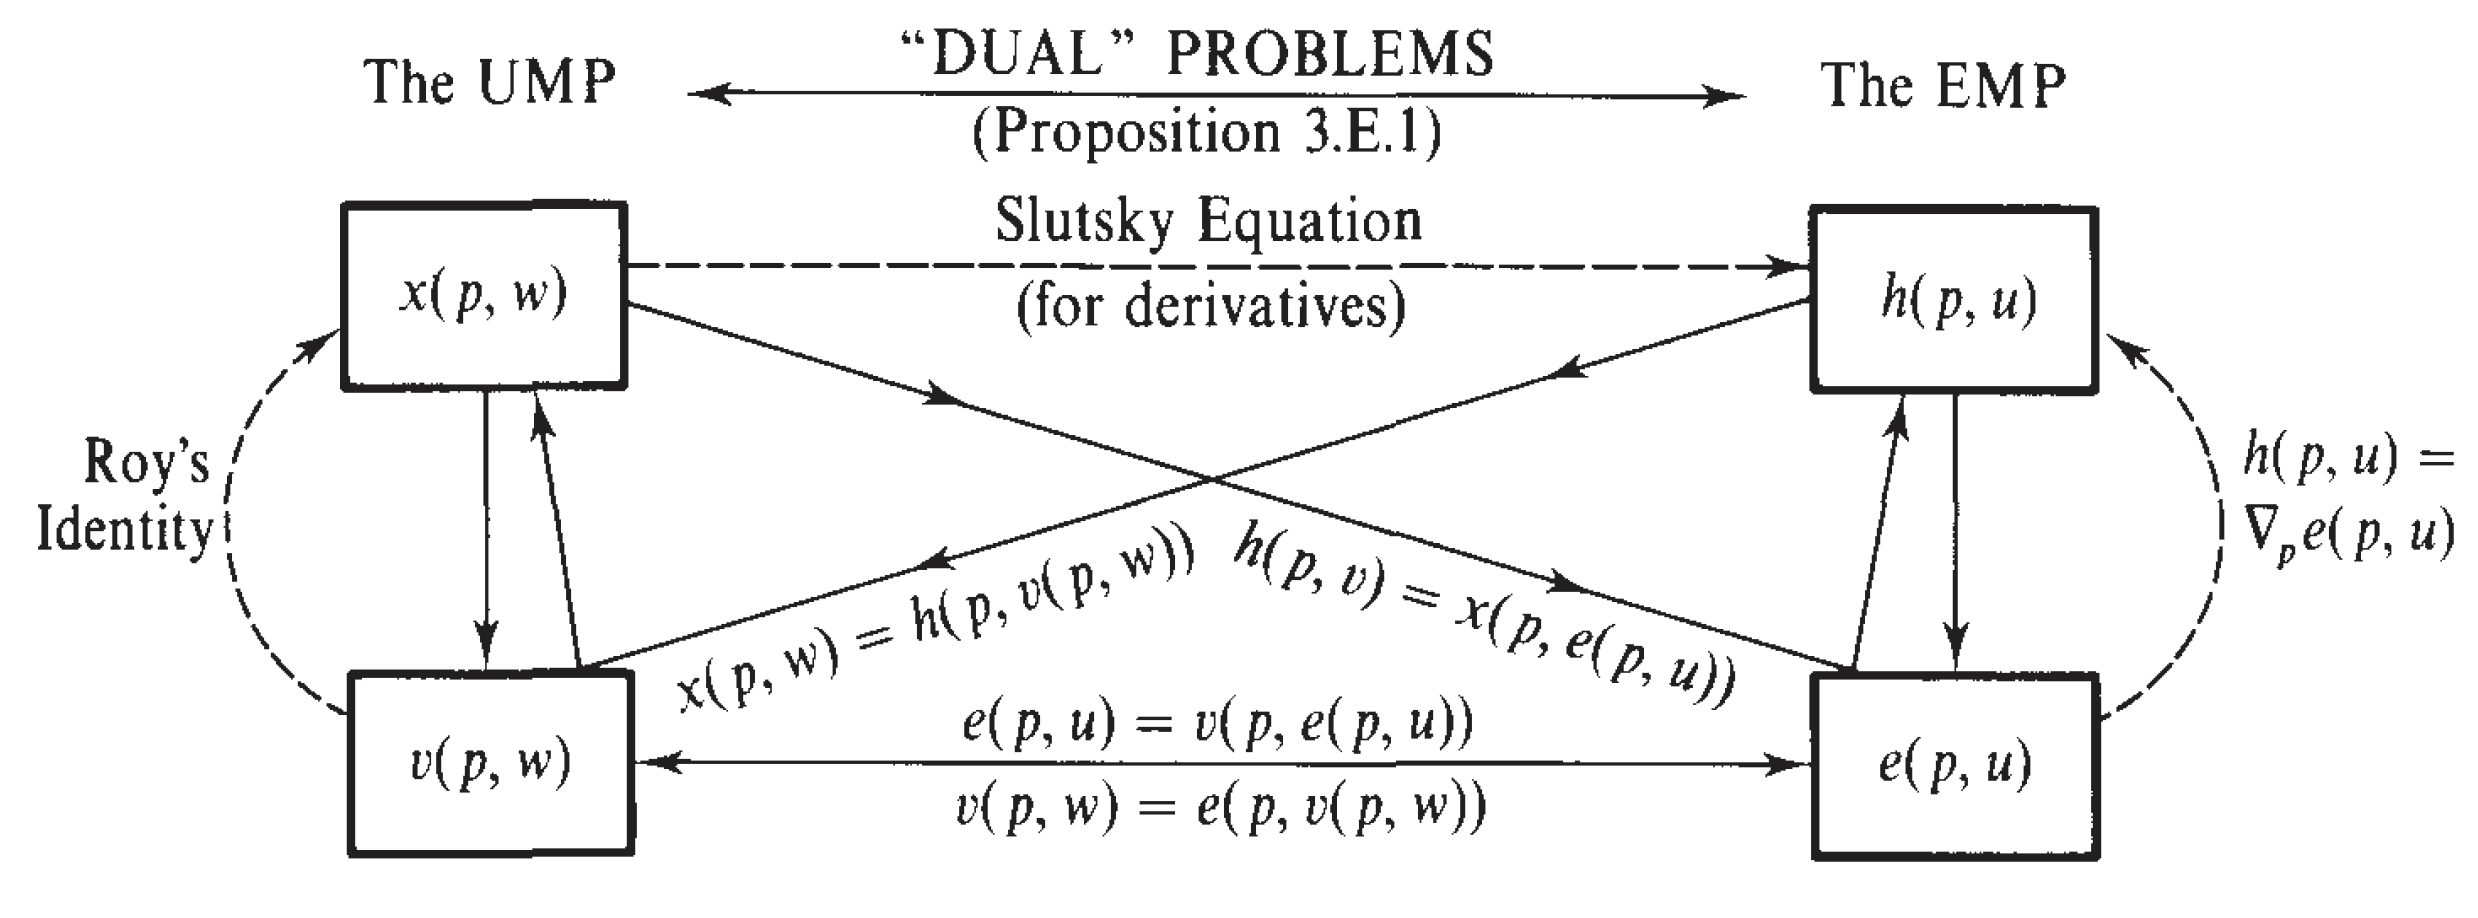
\includegraphics[width=1.0\linewidth]{figures/duality}
 				\caption{Fig. 3.G.3 in Mas-Colell: A Summary}
 			\end{figure}
 		
 		\subsection{Integrability}
 			\par \hl{TODO: this subsection needs revision.}
 			\begin{remark}[the Central Question]
 				Given a continuously differentiable demand function $x(p, w)$ satisfying homogenous of degree zero, Walras' law, and possessing negative semidefinite substitution matrix $S(p, w)$, can we find preferences rationalizing $x(p,w)$.
 			\end{remark}
 			
 			\begin{proposition}
 				Suppose the demand $x(p, w)$ satisfying the weak axiom, homogeneity of degree zero and Walras' law, then it can be rationalized by preferences \ul{if and only if} it has a symmetric substitution matrix $S(p, w)$.
 			\end{proposition}
 			
 			\subsubsection{Recovering Preferences from the Expenditure Function}
 			
 			\paragraph{Construction}For each utility level $u$, we can construct a \textbf{at-least-as-good-as set} $V_u \subset \R^L$ such that \ul{$e(p, u)$ is the minimal expenditure required for the consumer to purchase a bundle in $V_u$ at all price $p \gg 0$}. That's $V_u$ satisfies
 			\begin{equation}
 				\forall p \gg 0,\ e(p, u) = \min_{x \geq 0} p \cdot x\ s.t.\ x \in V_u
 			\end{equation}
 			
 			\begin{proposition}[3.H.1]
 				Suppose that $e(p, u)$ is strictly increasing in $u$ and is continuous, increasing, homogeneous of degree one, concave, and differentiable in $p$. Then, for every utility level $u$, $e(p, u)$ is the expenditure associated with at-least-as-good-as set
 				\begin{equation}
 					V_{u}=\left\{x \in \mathbb{R}_{+}^{L} : p \cdot x \geq e(p, u) \text { for all } p \gg 0\right\}
 				\end{equation}
 				That is, $e(p, u) = \min\{p\cdot x: x \in V_u\}\ \forall p \gg 0$.
 			\end{proposition}
 			
 			\par Then, for each $u > u(0)$, we can construct such $V_u$ and define $\pref$ on $X = \R^L_+$ with $V_u$. That's, for a given $x \in \R^L_+$ such that $u(x) \leftarrow \overline{u}$, then for each $y \in \R^L_+$,
 			\begin{equation}
 				y \pref x \iff y \in V_{\overline{u}}
 			\end{equation}
 			
 			\subsubsection{Recovering the Expenditure Function from Demand}
 			\paragraph{Construction} Suppose $x(p, w)$ is known, and by Shephard's lemma, expenditure function $e(p, w)$ can be solved from the system of partial differential equations
 			\begin{equation}
 				\begin{array}{l}{\frac{\partial e(p)}{\partial p_{1}}=x_{1}(p, e(p))} \\ {\vdots} \\ {\frac{\partial e(p)}{\partial p_{L}}=x_{L}(p, e(p))}\end{array}
 			\end{equation}
 			and initial conditions.
 			
 			\begin{proposition}
 				The necessary and sufficient condition for the recovery of an underlying expenditure function is the symmetry and negative semi-definiteness of the Slutsky matrix.
 			\end{proposition}
 		
 		\subsection{Welfare Evaluation of Economic Changes}
 			\paragraph{Context}We assume that the consumer has a fixed wealth level $w > 0$ and that the price vector is initially $p^0$. We wish to evaluate the impact on the consumer's welfare of a change from $p^0$ to a new price vector $p^1$.
 			
 			\begin{definition}
 				\textbf{Money metric} indirect utility functions measure welfare change expressed in dollar units. A money metric can be formed at an \ul{arbitrary price vector} $\overline{p} \gg 0$, and the welfare change expressed in dollar units is
 				\begin{equation}
 					e\left(\overline{p}, v\left(p^{1}, w\right)\right)-e\left(\overline{p}, v\left(p^{0}, w\right)\right)
 				\end{equation}
 			\end{definition}
 			
 			\begin{definition}
 				Let $u^0 = v(p^0, w)$, $u^1 = v(p^1, w)$, and noting that $e(p^0, u^0) = e(p^1, u^1) = w$.
 				When $\overline{p} = p^0$, the money metric is called \textbf{equivalence variation}
 				\begin{equation}
 					EV \left(p^{0}, p^{1}, w\right)=e\left(p^{0}, u^{1}\right)-e\left(p^{0}, u^{0}\right)=e\left(p^{0}, u^{1}\right)-w
 				\end{equation}
 				when $\overline{p} = p^1$, then it is referred to as
 				\begin{equation}
 					CV\left(p^{0}, p^{1}, w\right)=e\left(p^{1}, u^{1}\right)-e\left(p^{1}, u^{0}\right)=w-e\left(p^{1}, u^{0}\right)
 				\end{equation}
 			\end{definition}
 			
 			\begin{remark}[Interpretation of EV]
 				The equivalent variation can be thought of as the dollar amount that the consumer would be indifferent about accepting in lieu of the price change; that is, it is the change in her wealth that would be equivalent to the price change in terms of its welfare impact (so it is negative if the price change would make the consumer worse off). Therefore,
 				\begin{equation}
 					v(p^0, w+EV) = u^1
 				\end{equation}
 			\end{remark}
 			
 			\begin{remark}[interpretation of CV]
 				The compensating variation, on the other hand, measures the net revenue of a planner who must compensate the consumer for the price change after it occurs, bringing her back to her original utility level $u^0$ (Hence, the compensating variation is negative if the planner would have to pay the consumer a positive level of compensation because the price change makes her worse off.)
 				\begin{equation}
 					v\left(p^{1}, w-C V\right)=u^{0}
 				\end{equation}
 			\end{remark}
 			
 			\begin{proposition}
 				Suppose $p_1$ changes from $p_1^0$ to $p_1^1$, and $p^0_\ell = p^1_\ell = \overline{p}_\ell\ \forall \ell \neq 1$,
 				\begin{align}
 					EV\left(p^{0}, p^{1}, w\right) &=e\left(p^{0}, u^{1}\right)-w \\ 
 					&=e\left(p^{0}, u^{1}\right)-e\left(p^{1}, u^{1}\right) \\
 					&=\int_{p_{1}^{1}}^{p_{1}^{0}} h_{1}\left(p_{1}, \overline{p}_{-1}, u^{1}\right) d p_{1}
 				\end{align}
 				Similarly
 				\begin{align}
	 				CV\left(p^{0}, p^{1}, w\right) &= w - e(p^1, u^0) \\
	 				&= e(p^0, u^0) - e(p^1, u^0) \\
	 				&=\int_{p_{1}}^{p_{1}^{\circ}} h_{1}\left(p_{1}, \overline{p}_{-1}, u^{0}\right) d p_{1}
 				\end{align}
 			\end{proposition}
 			
 			\begin{remark}
 				However, if there is no wealth effect for good 1 (e.g., if the underlying preferences are quasilinear with respect to some good $\ell \neq 1$), the CV and EV measures are the same.
 			\end{remark}
 			
 			\begin{definition}
 				The value of area lying between $p_0^1$ and $p_1^1$ to the left of the market (Walrasian) demand curve for good 1, $\int_{p_1^1}^{p_1^0} x_1(p_1, \overline{p}_{-1}, w)\ dp_1$, measures the change in \textbf{Marshallian consumer surplus}. Such welfare measure is a special case of money metric when the wealth effects are absent.
 			\end{definition}
 			
 			\begin{definition}
 				Suppose the government imposes commodity tax of $t$ for each unit of good 1, let $T$ denote the amount of tax collected, then the \textbf{deadweight loss of commodity taxation} is 
 				\begin{align}
 					(-T)-E V\left(p^{0}, p^{1}, w\right) &=e\left(p^{1}, u^{1}\right)-e\left(p^{0}, u^{1}\right)-T \\
 					&=\int_{p_{1}^{0}}^{p_{1}^{0}+t} h_{1}\left(p_{1}, \overline{p}_{-1}, u^{1}\right) d p_{1}-t h_{1}\left(p_{1}^{0}+t, \overline{p}_{-1}, u^{1}\right) \\
 					&=\int_{p_{1}^{0}}^{p_{1}^{0}+t}\left[h_{1}\left(p_{1}, \overline{p}_{-1}, u^{1}\right)-h_{1}\left(p_{1}^{0}+t, \overline{p}_{-1}, u^{1}\right)\right] d p_{1}
 				\end{align}
 				It measures the extra amount by which the consumer is made worse off by commodity taxation above what is necessary to raise the same revenue through a lump-sum tax.
 			\end{definition}
 			
 			\subsubsection{Welfare Analysis with Partial Information}
 			
 			\begin{proposition}[3.I.1]
 				Suppose that the consumer has a locally nonsatiated rational preference relation $\pref$. If $(p^1-p^0) \cdot x^0 < 0$, then the consumer is strictly better off under price-wealth situation $(p^1, w)$ than $(p^0, w)$.
 			\end{proposition}
 			
 			\begin{proof}
 				By Walras' law, $p^0 \cdot x^0 = w$. Therefore, $x^0 \in B_{p_1, w}^{int}$. Because $x^0$ is in the interior of budget set, so $x^0 \neq x^1$ by local nonsatiation. As a result, $x^1 \succ^* x^0$ is revealed.
 			\end{proof}
 			
 			\begin{proposition}[3.I.2]
 				Suppose that the consumer has a differentiable expenditure function. then if $\left(p^{1}-p^{0}\right) \cdot x^{0}>0$, there is a sufficiently small $\overline{\alpha} \in (0, 1)$ such that for all $\alpha < \overline{\alpha}$, we have $\left(p^{1}-p^{0}\right) \cdot x^{0}>0$, and so the consumer is strictly better off under price-wealth situation $(p^0, w)$ than under $\left((1-\alpha) p^{0}+\alpha p^{1}, w\right)$
 			\end{proposition}
 			
 			\begin{definition}
 				The \textbf{area variation} measure (AV) provides an estimate of welfare change when only Walrasian demand is observable
 				\begin{equation}
 					A V\left(p^{0}, p^{1}, w\right)=\int_{p_{1}^{1}}^{p_{1}^{0}} x_{1}\left(p_{1}, \overline{p}_{-1}, w\right) d p_{1}
 				\end{equation}
 			\end{definition}
 			
 			\begin{remark}
 				When there are no wealth effects, $AV=EV=CV$.
 			\end{remark}
 			
 			\begin{remark}
 				Marshall argued that if a good is just one commodity among many, then because one extra unit of wealth will spread itself around, the wealth effect for the commodity is bound to be small; therefore, no significant errors will be made by evaluating the welfare effects of price changes for that good using the area measure.
 			\end{remark}
 			
 			\begin{remark}
 				So when $\Delta p$ is small, the error involved using the area variation measure becomes small as a fraction fo the true welfare change, and therefore, can be used as an accurate approximation of the actual welfare change.
 			\end{remark}
 			
 		\subsection{The Strong Axiom of Revealed Preference}
 			\begin{definition}[3.J.1]
 				The market demand function $x(p, w)$ satisfies the \textbf{strong axiom of revealed preference} (the SA) if for any sequence
 				\begin{equation}
 					\left(p^{1}, w^{1}\right), \ldots,\left(p^{N}, w^{N}\right)
 				\end{equation}
 				with $x\left(p^{n+1}, w^{n+1}\right) \neq x\left(p^{n}, w^{n}\right)$ for all $n \leq N-1$, we have 
 				\begin{equation}
 					\underbrace{p^{n} \cdot x\left(p^{n+1}, w^{n+1}\right) \leq w^{n}}_{x^n \succ^* x^{n+1} \tx{ revealed}}
 					\ \forall n \leq N - 1
 					\implies p^{N} \cdot x\left(p^1, w^1\right)>w^{N}
 				\end{equation}
 			\end{definition}
 			
 			\begin{proposition}[3.J.1]
 				If the Walrasian demand function $x(p, w)$ satisfies the strong axiom of revealed preference then there is a rational preference relation $\pref$ that rationalizes $x(p, w)$, that is, such that for all $(p, w)$, 
 				\begin{equation}
 					x(p, w) \succ y\ \forall y \in B_{p, w}\ s.t.\ y \neq x(p, w)
 				\end{equation}
 			\end{proposition}
 			
			\begin{proposition}[1.D.2 (\hl{WARP $\to$ Rational})]
				If $(\mathscr{B}, C(\cdot))$ is a choice structure such that
				\begin{enumerate}[(i)]
					\item The weak axiom is satisfied;
					\item $\mathscr{B}$ includes all subsets of $X$ up to three elements.
				\end{enumerate}
				Then there is a rational preference relation $\pref$ that rationalizes $C(\cdot)$ relative to $\mathscr{B}$.
			\end{proposition}
 			
 			\begin{remark}
 				Proposition 3.J.1 tells us that a choice-based theory of demand founded on the strong axiom is essentially equivalent to the preference-based theory of demand presented in this chapter.
 			\end{remark}
 	
 	\section{Chapter 4. Aggregate Demand}
 		\subsection{Aggregate Demand and Aggregate Wealth}
	 		\paragraph{Context}Suppose there are $I$ consumers with rational preference relations $\pref_i$ and corresponding Walrasian demand function $x_i(p, w_i)$. We want to write the \textbf{aggregate demand}
	 		\begin{equation}
	 			x\left(p, w_{1}, \ldots, w_{I}\right)=\sum_{i=1}^{I} x_{i}\left(p, w_{i}\right)
	 		\end{equation}
	 		as a function of price level $p$ and aggregate wealth $\sum_i w_i$, but independent to the wealth distribution. Specifically, for any two wealth distribution $(w_i)$ and $(w_i')$,
	 		\begin{equation}
	 			\sum_i w_i = \sum_i w_i' \implies \sum_i x_i(p, w_i) = \sum_i x_i(p, w_i')
	 		\end{equation}
	 		
	 		\begin{proposition}
	 			The above property can be written using differential change in wealth $(d w_i)$ such that $\sum_i d w_i = 0$. Assuming the differentiability of Walrasian demand functions, the invariant condition is equivalent to 
	 			\begin{equation}
	 				\sum_{i} \frac{\partial x_{\ell i}\left(p, w_{i}\right)}{\partial w_{i}} d w_{i}=0 \quad \text { for every } \ell
	 			\end{equation}
	 			which holds \ul{if and only if}
	 			\begin{equation}
	 				\frac{\partial x_{\ell i}\left(p, w_{i}\right)}{\partial w_{i}}=\frac{\partial x_{\ell j}\left(p, w_{j}\right)}{\partial w_{j}}
	 			\end{equation}
	 			for every commodity $\ell$, pair of individuals $i, j$, and all wealth distribution $(w_i)$.
	 		\end{proposition}
	 		
	 		\begin{proof}
	 			($\implies$) for given $\ell, i, j$, we can define $d\ve{w} := \ve{e}_i - \ve{e}_j$ and substitute it into the identity. \\
	 			($\impliedby$) if all partial derivatives with respect to $w$ are equal, we can partial them out from the summation, $\sum_{i} \frac{\partial x_{\ell i}\left(p, w_{i}\right)}{\partial w_{i}} d w_{i} = \eta^* \sum_i dw_i$. And because $\sum_i dw_i = 0$, $\sum_{i} \frac{\partial x_{\ell i}\left(p, w_{i}\right)}{\partial w_{i}} d w_{i}$.
	 		\end{proof}
	 		
	 		\begin{remark}
	 			The above proposition says aggregate demand is independent to the particular wealth distribution if the individual demand changes arising from any wealth redistribution across consumers will cancel out. Geometrically, the condition is equivalent to \emph{all consumers' wealth expansion paths are parallel string lines}.
	 		\end{remark}
	 		
	 		\begin{proposition}[4.B.1]
	 			A \ul{necessary and sufficient} condition for the set of consumers to exhibit parallel, straight wealth expansion paths at any price vector $p$ is that their preferences admit indirect utility functions of the \textbf{Gorman form} with the coefficients on $w_i$ identical for every consumer, that's,
	 			\begin{equation}
	 				v_{i}\left(p, w_{i}\right)=a_{i}(p)+b(p) w_{i}
	 			\end{equation}
	 		\end{proposition}
	 		
	 		\begin{definition}
	 			A family of functions $(w_1(p, w), \dots, w_I(p, w))$ with $\sum_i w_i(p, w) = w$ for all $(p, w)$ is called a \textbf{wealth distribution rule}.
	 		\end{definition}
	 		
	 		\begin{proposition}
	 			If the individual wealth levels are generated by a wealth distribution rule, we can always write the aggregate demand $x(p, w)$ as a function depends only on price and aggregate wealth.
	 		\end{proposition}
	 
	 \section{Chapter 5. Production}
	 	\subsection{Production Sets}
	 		\begin{definition}
	 			A \textbf{production vector}/\textbf{production plan} is a vector $y \in \R^L$ that describes the net outputs of $L$ commodities from a production process. Where positive numbers denote outputs and negative numbers denote inputs. The set of all \emph{technologically possible} production plans is defined as the \textbf{production set} $Y \subset \R^L$.
	 		\end{definition}
	 		
	 		\begin{remark}
	 			The set of feasible production plans is limited first and foremost by technological constraints. However, in any particular model, legal restrictions or prior contractual commitments may also contribute to the determination of the production set.
	 		\end{remark}
	 		
	 		\begin{definition}
	 			The \textbf{transformation function} $F: \R^L \to \R$ associated with production plan $Y$ is defined such that
	 			\begin{equation}
	 				Y=\left\{y \in \mathbb{R}^{L} : F(y) \leq 0\right\}
	 			\end{equation}
	 			and $F(y)$ if and only if $y \in \partial\ Y$. The set $\left\{y \in \mathbb{R}^{L} : F(y)=0\right\}$ is called the \textbf{transformation frontier}.
	 		\end{definition}
	 		
	 		\begin{definition}
	 			The \textbf{marginal rate of transformation (MRT) of good $\ell$ for good $k$ at $\overline{y}$} is defined as 
	 			\begin{equation}
	 				M R T_{\ell k}(\overline{y}) := \frac{\partial F(\overline{y}) / \partial y_{\ell}}{\partial F(\overline{y}) / \partial y_{k}} \left ( = \frac{dy_k}{dy_\ell} \right )
	 			\end{equation}
	 			it is a measure of how much the (net) output of good $k$ can increase if the firm decreases the (net) output of good $\ell$ by one marginal unit.
	 		\end{definition}
	 		
	 		\begin{definition}
	 			For single-output technologies with distinct inputs and output, the \textbf{production function} $f(z)$ is defined as the maximum amount $q$ of output that can be produced using input amounts $(z_1, \cdots, z_{L-1}) \geq 0$. So the production set generated by $f$ is 
	 			\begin{equation}
	 				Y=\left\{\left(-z_{1}, \ldots,-z_{L-1}, q\right) : q-f\left(z_{1}, \ldots, z_{L-1}\right) \leq 0 \land \left(z_{1}, \ldots, z_{L-1}\right) \geq 0\right\}
	 			\end{equation}
	 		\end{definition}
	 		
	 		\begin{definition}
	 			The \textbf{marginal rate of technical substitution (MRTS) of input $\ell$ for input $k$ at $\overline{z} \geq 0$} is defined to be
	 			\begin{equation}
	 				MRTS_{\ell k}(\overline{z}) := \frac{\partial f(\overline{z}) / \partial z_{\ell}}{\partial f(\overline{z}) / \partial z_{k}}
	 			\end{equation}
	 		\end{definition}
	 		
	 		\begin{assumption}
	 			Common properties of production sets assumed are
	 			\begin{enumerate}[(i)]
	 				\item $Y \neq \varnothing$;
	 				\item $Y$ is closed (\emph{primarily for technical issues});
	 				\item \emph{No free lunch}: $y \in Y \land y \geq 0 \implies y = 0$, more succinctly, $Y \cap \R^L_+ \subset \{0\}$;
	 				\item \emph{Possibility of inaction}: $0 \in Y$;
	 				\item \emph{Free disposal}: $Y - \R^L_+ \subset Y$;
	 				\item \emph{Irreversibility}: $\forall y \in Y \backslash \neq 0, -y \notin Y$;
	 				\item \emph{Non-increasing returns to scale}: $y \in Y \land \alpha \in [0, 1] \implies  \alpha y \in Y$;
	 				\item \emph{Non-decreasing returns to scale}: $y \in Y \land \alpha \geq 1 \implies \alpha y \in Y$;
	 				\item \emph{Constant returns to scale}: $y \in Y \land \alpha \geq 0 \implies \alpha y \in Y$, therefore, $Y$ is a cone;
	 				\item \emph{Additivity/Free entry}: $Y + Y \subset Y$;
	 				\item \emph{Convexity}: $Y$ is convex;
	 				\item $Y$ is a convex cone: $\forall y_1, y_2 \in Y, \alpha, \beta \geq 0,\ \alpha y_1 + \beta y_2 \in Y$.
	 			\end{enumerate}
	 		\end{assumption}
	 		
	 		\begin{definition}
	 			A subset $C$ of a vector space $V$ is a \textbf{cone} (or sometimes called a linear cone) if $\forall x \in C, \alpha \geq 0,\ \alpha x \in C$.
	 		\end{definition}
	 		
	 		\begin{proposition}[Exercise 5.B.2]
	 			For single-output technologies with distinct inputs and output, $Y$ satisfies constant return to scale \ul{if and only if} $f(\cdot)$ is homogenous of degree 1.
	 		\end{proposition}
	 		
	 		\begin{proposition}[5.B.1]
	 			The production set $Y$ is additive and satisfies the non-increasing returns condition \ul{if and only if} it is a convex cone.
	 		\end{proposition}
	 		
	 		\begin{proposition}[5.B.2, adding the missing entrepreneurship input factor]
	 			For any convex production set $Y \subset \R^L$ with $0 \in Y$, there is a constant returns, convex production set $Y' \subset \R^{L+1}$ such that
	 			\begin{equation}
	 				Y = \{y \in \R^L: (y, -1) \in Y'\}
	 			\end{equation}
	 		\end{proposition}
	 		
	 		\begin{remark}
	 			In a competitive environment, the return to the entrepreneurial factor is the firm's profit.
	 		\end{remark}

	 	\subsection{Profit Maximization and Cost Minimization}
	 		\begin{assumption}[price-taking assumption]
	 			Assuming the prices quoted for the $L$ goods, $p \gg 0$, are independent of the production plans of the firm.
	 		\end{assumption}
	 		
	 		\begin{assumption}
	 			We assume that the firm's production set $Y$ satisfies the \emph{non-emptiness}, \emph{closedness}, and \emph{free disposal}.
	 		\end{assumption}
	 		
	 		\subsubsection{The Profit Maximization Problem}
	 		\begin{definition}[PMP]
	 			\begin{gather}
	 				\max_{y \in \R^L}\ p \cdot y\ s.t.\ y \in Y
	 			\end{gather}
	 			equivalently
	 			\begin{gather}
	 				\max_{y \in \R^L}\ p \cdot y\ s.t.\ F(y) \leq 0
	 			\end{gather}
	 			define the \textbf{profit function} and \textbf{supply correspondence} as 
	 			\begin{align}
	 				\pi(p) &:= \max\{p \cdot : y \in Y\} \\
	 				y(p) &:= \argmax\{p \cdot : y \in Y\}
	 			\end{align}
	 			If the transformation function $F(\cdot)$ is differentiable, then the necessary condition for $y^* \in y(p)$ is
	 			\begin{equation}
	 				p = \lambda \nabla F (y^*)
	 			\end{equation}
	 		\end{definition}
	 		
	 		\begin{definition}[PMP with single-output technology]
	 			Suppose the input and output sets are disjoint. Let $f: \R^{L-1}_+ \to \R_+$ denote the production function, let $w$ and $p$ denote the prices of inputs and the output commodity respectively. The PMP can be written as 
	 			\begin{equation}
	 				\max_{z \geq 0} p f(z) - w \cdot z
	 			\end{equation}
	 			the necessary conditions for $z^* \in \argmax$ are
	 			\begin{equation}
		 			\begin{cases}
		 				p\ \nabla f(z^*) \leq w \\
		 				\left[p\ \nabla f(z^*) - w\right] \odot z^* = 0
		 			\end{cases}
	 			\end{equation}
	 			\emph{Interpretation: the marginal product of every input $\ell$ actually used must equal its price in terms of output, $w_\ell / p$}.
	 		\end{definition}
	 		
	 		\begin{proposition}[5.C.1]
	 			Suppose $\pi(p)$ and $y(p)$ are the profit function and supply correspondence with production set $Y$. Further, suppose $Y$ is closed and satisfies the free disposal property. Then
	 			\begin{enumerate}[(i)]
	 				\item $\pi$ is homogeneous of degree one;
	 				\item $\pi$ is convex;
	 				\item If $Y$ is convex, then $Y = \{y \in \R^L: p \cdot y \leq \pi (p)\ \forall p \gg 0$;
	 				\item $y$ is homogeneous of degree zero;
	 				\item If $Y$ is convex, then $y(p)$ is a convex set for all $p$. If $Y$ is strictly convex, then $y(p)$ is a singleton (if nonempty);
	 				\item (\textbf{Hotelling's Lemma}) If $y(\overline{p})$ is a singleton, then $pi$ is differentiable at $p$ and $\nabla \pi (\overline{p}) = y(\overline{p})$;
	 				\item (\textbf{Lay of Supply}) If $y$ is a function differentiable at $\overline{p}$, then $Dy(\overline{p})=D^2 \pi(\overline{p})$ is a symmetric and positive semidefinite matrix with $Dy(\overline{p}) \overline{p})=0$. Where $Dy$ is called the \textbf{supply substitution matrix}.
	 			\end{enumerate}
	 		\end{proposition}
	 		
	 		\begin{proposition}[Law of Supply]
	 			Discrete case:
	 			\begin{equation}
	 				(p-p') \cdot (y-y') \geq 0
	 			\end{equation}
	 			Differential case, when $p = \overline{p}$ and $y = y(\overline{p})$:
	 			\begin{equation}
	 				dp \underbrace{Dy(p) dp}_{dy} = dp \cdot dy \geq 0
	 			\end{equation}
	 		\end{proposition}
	 		
	 		\subsubsection{Cost Minimization}
	 		\begin{definition}[CMP]
	 			Suppose the firm has a single-output technology, where input and output sets are disjoint. Let $(w, p) \gg 0$ denote the prices of inputs and the output. For each output level $q \geq 0$, the cost minimization problem is 
	 			\begin{equation}
	 				\min_{z \geq 0} w \cdot z\ s.t.\ f(z) \geq q
	 			\end{equation}
	 			The value function $c(w, q)$ is called the \textbf{cost function} and the solution set $z(w, q)$ is known as the \textbf{conditional factor demand correspondence}. The necessary conditions for $z^* \in z(w, q)$ are
	 			\begin{equation}
	 				\begin{cases}
	 					w \geq \lambda \nabla f(z^*) \\
	 					\left[w - \lambda \nabla f(z^*) \right] \odot z^* = 0
	 				\end{cases}
	 			\end{equation}
	 			By the envelope theorem, $\lambda^* = \pd{c(z^*, q)}{q}$, which can be interpreted as the marginal value of relaxing the constraint $f(z^*) \geq q$. Therefore, $\lambda$ is the \emph{marginal cost of production}.
	 		\end{definition}
	 		
	 		\begin{proposition}[5.C.2]
	 			Suppose that $c(w, q)$ and $z(w, q)$ are the cost function and conditional factor demand correspondence corresponding to a single-output technology $Y$ with production function $f$. Suppose $Y$ is closed and satisfies the free disposal property. Then
	 			\begin{enumerate}[(i)]
	 				\item $c$ is homogeneous of degree one in $w$ and nondecreasing in $q$;
	 				\item $c$ is a concave function of $w$;
	 				\item If the sets $\{z\geq0:f(z)\geq q\}$ are convex for every $q$, then $Y=\{(-z, q): w \cdot z \geq c(w, q)\ \forall w \gg 0\}$;
	 				\item $z$ is homogenous of degree zero in $w$;
	 				\item If the set $\{z \geq 0: f(z) \geq q\}$ is convex, then $z(w, q)$ is a convex set. If $\{z \geq 0: f(z) \geq q\}$ is strictly convex, then $z(w, q)$ is a singleton;
	 				\item (\textbf{Shepard's Lemma}) If $z(\overline{w}, q)$ is a singleton, then $c$ is differentiable with respect to $w$ at $\overline{w}$, and $\nabla_w c(\overline{w}, q) = z(\overline{w}, q)$;
	 				\item If $z$ is differentiable at $\overline{w}$ then $D_w z (\overline{w}, q) = D^2_w (\overline{w}, q)$ is a symmetric and negative semidefinite matrix with $D_w z (\overline{w}, q) \overline{w} = 0$;
	 				\item If $f$ is homogeneous of degree one (i.e. constant return to scale), then $c$ and $z$ are homogenous of degree one in $q$;
	 				\item If $f$ is concave, then $c$ is a convex function of $q$.
	 			\end{enumerate}
	 		\end{proposition}
	 		
	 		\begin{corollary}
	 			Alternative form of CMP, determining the profit-maximizing production level
	 			\begin{equation}
	 				\max_{q \geq 0} p q - c(w, q)
	 			\end{equation}
	 			where the necessary conditions for $q^* \in \argmax$ are
	 			\begin{equation}
	 				p \leq \pd{c(w, q^*)}{q}\tx{ with equality if } q^* > 0
	 			\end{equation}
	 			\emph{At an interior optimum, price equals marginal cost}. Note that if $c$ is convex in $q$ (i.e. $p q - c(w, q)$ is concave in q), the the necessary condition is also sufficient.
	 		\end{corollary}
	 
	 	\subsection{The Geometry of Cost and Supply in the Single-Output Case}
	 		\begin{definition}
	 			The cost function excluding any prior input commitments is called the \textbf{long-run cost function}.
	 		\end{definition}
	 		
	 		\begin{remark}
	 			Suppose input $z_k$ is fixed at $\overline{z}_k$, in the short run, then for each $q \geq 0$, the \textbf{short-run cost function} is defined as
	 			\begin{equation}
	 				C(q|\overline{z}_k) := \min_{z \geq 0}\{w\cdot z: f(z) \geq q, z_2=\overline{z}_2\}
	 			\end{equation}
	 			the corresponding long run cost function at $q$ is defined as 
	 			\begin{equation}
	 				C(q) := \min_{z \geq 0}\{w\cdot z: f(z) \geq q\}
	 			\end{equation}
	 			given the relaxation of constraint, for all $q \geq 0$, $C(q) \leq C(q|\overline{z}_k)$. Geometrically, $C(\cdot)$ is the \emph{lower envelope} of the family of short-run cost functions $\{C(q|\overline{z}_k): \overline{z}_k \geq 0\}$.
	 		\end{remark}
	 		
	 	\subsection{Aggregation}
	 		\begin{remark}
	 			The absence of budget constraint in the profit maximization implies that individual supply is not subject to wealth effects. As prices change, there are only substitution effects along the production frontier.
	 		\end{remark}
	 		
	 		\begin{definition}
	 			Suppose there are $J$ production units in the economy with production set $(Y_j)$. Assuming each $Y_j$ is nonempty, closed, and satisfies the free disposal property. Then the \textbf{aggregate supply correspondence} is defined as
	 			\begin{equation}
	 				y(p)=\sum_{j=1}^{J} y_{j}(p)=\left\{y \in \R^{L} : y=\sum_{j} y_{j} \tx { where } y_{j} \in y_{j}(p),\ \forall j=1, \cdots, J\right\}
	 			\end{equation}
	 		\end{definition}
	 		
	 		\begin{proposition}
	 			If every $y_j$ is single valued, since $Dy_j(p)$ is symmetric and positive semidefinite, then $D_y(p)$ is also symmetric and positive semidefinite.
	 		\end{proposition}
	 		
	 		\begin{proposition}[Law of supply in the aggregate]
	 			By adding over the \emph{lay of individual supply}, we have 
	 			\begin{equation}
	 				(p-p') \cdot \left[y(p)-y(p')\right] \geq 0
	 			\end{equation}
	 		\end{proposition}
	 		
	 		\begin{definition}
	 			The \textbf{aggregate production set} is defined as
	 			\begin{equation}
	 				Y := \sum_j Y_j = \left\{y \in \R^L: y = \sum_j y_j \tx{ where } y_j \in Y_j,\ \forall  j = 1, \cdots, J \right\}
	 			\end{equation}
	 		\end{definition}
	 		
	 		\begin{proposition}[5.E.1]
	 			For all $p \gg 0$, we have 
	 			\begin{enumerate}[(i)]
	 				\item $\pi^*(p) = \sum_j \pi_j (p)$;
	 				\item $y^*(p) = \sum_j y_j (p) = \left\{\sum_j y_j: y_j \in y_j(p)\ \forall j \right\}$.
	 			\end{enumerate}
	 			\emph{Interpretation: the aggregate profit obtained by each production unit maximizing profit separately taking prices as given is the same as that which would be obtained if they were to coordinate their actions in a joint profit maximizing decision.} Therefore, to find the solution of the aggregate profit maximization problem for given prices $p$, it is enough to add the solutions of the corresponding individual problems. Moreover, given the minimizing aggregate output $q = \sum_j q_j$, the total cost $c(w, q)$ is exactly the value of \textbf{aggregate cost function} (the cost function corresponding to the aggregate production set $Y$). Thus, \emph{the allocation of production of output level $q$ among the firms is cost minimizing}. As a result, $q(p)$ satisfies necessary conditions $p \leq c'(q)$ and $(p - c'(q))q = 0$.
	 		\end{proposition}
	 	
	 	\subsection{Efficient Production}
	 		\begin{definition}[5.F.1]
	 			A production vector $y \in Y$ is \textbf{efficient} if there is no $y' \in Y$ such that $y' \geq y$ and $y' \neq y$. That is, $Y \cap (\{y\} + \R^L_+) = \{y\}$.
	 		\end{definition}
	 		
	 		\begin{proposition}[5.F.1, A simplified version of the first fundamental theorem of welfare economics]
	 			If $y \in Y$ is profit maximizing for some $p \gg 0$, then $y$ is efficient. \emph{Interpretation: if a collection of firms each independently maximizes profits with respect to the same fixed price vector $p \gg 0$, then the aggregate production is socially efficient.}
	 			\begin{equation}
	 				\tx{Competitive Equilibrium} \implies \tx{Pareto Optimal}
	 			\end{equation}
	 		\end{proposition}
	 		
	 		\begin{remark}
	 			The above proposition is valid even if the production set is non-convex.
	 		\end{remark}
	 		
	 		\begin{proposition}[5.F.2, A simplified version of the second fundamental theorem of welfare economics]
	 			Suppose $Y$ is convex. Then every efficient production $y \in Y$ is a profit-maximizing production for some nonzero price vector $p \geq 0$.
	 			\begin{equation}
	 			\tx{Pareto Optimal}\overset{\tx{reallocation}}{\implies} \tx{Competitive Equilibirum}
	 			\end{equation}
	 		\end{proposition}
	 		
	 	\subsection{Remarks on the Objectives of the Firm}
	 		\begin{remark}
	 			Suppose that firm with production set $Y$ is owned by consumer with allocation of owner ship $(\theta_i) \geq 0$ such that $\sum_i \theta_i = 1$. All profit is given back to owners according to the their shares of the firm. The owners of the firm are consumers and trying to solve the UMP
	 			\begin{equation}
	 				\max_{x_i} u_i(x_i)\ s.t.\ p \cdot x_i \leq w_i + \theta_i p \cdot y
	 			\end{equation}
	 			Where $w_i$ is the nonprofit wealth of consumer $I$. At any fixed price vector $p \gg 0$, the consumer owners unanimously prefer that the firm implement a production plan $y' \in Y$ instead of $y \in Y$ whenever $p\cdot y' > p\cdot y$ (as such change relaxes the budget constraint and provides marginal utility $\lambda^*$). Hence, we conclude that if we maintain the assumption of price-taking behaviour, all owners would agree, whatever their utility functions, to instruct the manager of the firm to maximize profits. Therefore, firms' profit maximization behaviour is justified.
	 		\end{remark}
	 		
	 		\begin{remark}
	 			Three assumptions are crucial for above justification:
	 			\begin{enumerate}[(i)]
	 				\item Price-taker assumption: \emph{if the prices of inputs are increased due to the increased amount of output, and the same inputs provide substantive utilities. Then the solution to UMP may lead to a production level below the optimal output level, to keep the inputs relatively cheap};   
	 				\item Profits are not uncertain;
	 				\item Managers can be controlled by owners.
	 			\end{enumerate}
	 		\end{remark}
	 		
	\section{Notes on Comparative Statics}
		\subsection{Univariate Case}
			\begin{definition}
				Let $A, B \subseteq X$, then $A$ is (weakly) dominated by $B$ in the \textbf{strong set order} sense, denoted as $A \leq_S B$, if 
				\begin{equation}
					\forall (a, b) \in A \times B,\ \min\{a, b\} \in A \land \max\{a, b\} \in B
				\end{equation}
			\end{definition}
			
			\begin{definition}
				A correspondence $x: \R \rightrightarrows \R$ is \textbf{(weakly) increasing} if 
				\begin{equation}
					t < t' \implies x(t) \leq_S x(t')
				\end{equation}
			\end{definition}
			
			\begin{remark}
				When $x$ is a function, then above definition collapses to the conventional definition of increasing functions.
			\end{remark}
		
			\begin{definition}[Single Crossing Condition (Milgrom and Shannon)]
				A family of functions $f(\cdot, t): D \subset \R^2 \to \R$ indexed by $t$ is ordered by the \textbf{single crossing condition} if for every $t < t'$ and $x < x'$,
				\begin{align}
					\overbrace{f(x', t) - f(x, t)}^{\Delta^+_x(t)} \geq 0 \implies \overbrace{f(x', t') - f(x, t')}^{\Delta^+_x(t')} \geq 0 \\
					f(x', t) - f(x, t) > 0 \implies f(x', t') - f(x, t') > 0
				\end{align}
			\end{definition}
			
			\begin{theorem}
				Let 
				\begin{equation}
					x^*(t) := \argmax_x f(x, t)
				\end{equation}
				if the family $f(\cdot, t)$ is ordered by the single crossing condition, then $x^*(t)$ is increasing.
			\end{theorem}
			
			\begin{theorem}
				Let
				\begin{equation}
					x_Y^*(t) := \argmax_{x \in Y} f(x, t)
				\end{equation}
				then the following statements are equivalent
				\begin{enumerate}[(i)]
					\item The family $f(\cdot, t)$ is ordered by single crossing condition.
					\item For each $Y \subset \R$, each $t < t'$
					\begin{equation}
						x_Y^*(t) \leq_S x_Y^*(t')
					\end{equation}
				\end{enumerate}
			\end{theorem}
			
			\begin{definition}
				Function $f: \R^2 \to \R$ has \textbf{increasing differences} if $\forall x < x'$, the difference
				\begin{equation}
					\Delta^+_x(t) := f(x', t) - f(x, t)
				\end{equation}
				is (weakly) increasing in $t$. $f$ has strictly increasing differences if $\Delta^+_x(t)$ is strictly increasing in $t$.
			\end{definition}
			
			\begin{remark}
				Increasing differences is a stronger condition than the single crossing condition.
			\end{remark}
			
			\begin{theorem}
				Let 
				\begin{equation}
					x_Y^*(t) := \argmax_{x \in Y} f(x, t) + g(x)
				\end{equation}
				then the following statements are equivalent
				\begin{enumerate}[(i)]
					\item Function $f$ has increasing differences.
					\item $x_Y^*(t)$ is (weakly) increasing in $t$ for all functions $g$ and sets $Y$.
				\end{enumerate}
			\end{theorem}
			
			\begin{lemma}
				If $f$ is twice differentiable, then the family $f(\cdot, t)$ has increasing differences \ul{if and only if} $f_{xt} \geq 0\ \forall x, t$.
			\end{lemma}
			
		\subsection{Multivariate Case}
	
	\section{Chapter 6. Choice Under Uncertainty}
		\subsection{Expected Utility Theory}
			\begin{assumption}
	 			Let $C$ denote the set of all possible \emph{outcomes}/\emph{consequences} from one \emph{risky alternative}. For simplicity, we assume $C$ is finite, indexed by $n=1, \cdots, N$.
	 		\end{assumption}
	 		
	 		\begin{assumption}
	 			We assume that the probabilities of various outcomes arising from any chosen alternative are \emph{objectively known}.
	 		\end{assumption}
	 		
	 		\begin{definition}[6.B.1]
	 			A \textbf{simple lottery} $L$ is a list $(p_n)_n \geq 0$ such that $\sum_n p_n = 1$, where $p_n$ is interpreted as the probability of outcome $n$ occurring. \emph{That is, a lottery is a distribution on the outcome space}. If $p_n = 1$ for some $n$, then $L$ is said to be a \textbf{degenerate lottery}.
	 		\end{definition}
	 		
	 		\begin{remark}
	 			The set of all simple lotteries with $N$ outcomes is the $(N-1)$ dimensional simplex
	 			\begin{equation}
	 				\Delta := \left\{p \in \R^N: p_1 + \cdots + p_N = 1 \right\}
	 			\end{equation}
	 		\end{remark}
	 		
	 		\begin{definition}[6.B.2]
	 			Given $K$ simple lotteries $L_k = (p_n^k)$, and probabilities $(\alpha_k)$ with $\sum_k \alpha_k = 1$, the \textbf{compound lottery} $(L_k; \alpha_k)$ is the risky alternative that yields the simple lottery $L_k$ with probability $\alpha_k$ for each $k$.
	 		\end{definition}
	 		
	 		\begin{proposition}
	 			A compound lottery can be \textbf{reduced} into a simple lottery, the probability of outcome $n$ in the reduced lottery is
	 			\begin{equation}
	 				p_n = \alpha_1 p_n^1 + \cdots \alpha_k p_n^k
	 			\end{equation}
	 			Equivalently, with vector addition
	 			\begin{equation}
	 				L := \sum_{k=1}^K \alpha_k L_k \in \Delta
	 			\end{equation}
	 		\end{proposition}
	 		
	 		\begin{assumption}[Consequentialist Premise]
	 			We assume that for any risky alternative, only the reduced lottery over final outcomes is of relevance to the decision maker.
	 		\end{assumption}
	 		
	 		\begin{assumption}
	 			Let $\mathscr{L}$ denote the set of all simple lotteries over the set of outcomes $C$. We assume that the decision maker has a rational preference relation $\pref$ on $\mathscr{L}$.
	 		\end{assumption}
	 		
	 		\begin{definition}[6.B.3]
	 			The preference relation $\pref$ on the space of simple lotteries $\mathscr{L}$ is \textbf{continuous} if for any $L, L', L'' \in \mathscr{L}$, the set
	 			\begin{equation}
	 				\left\{\alpha \in[0,1] : \alpha L + (1-\alpha) L' \pref L''\right\} \subset[0,1]
	 			\end{equation}
	 			and 
	 			\begin{equation}
	 				\left\{\alpha \in[0,1] : L'' \pref \alpha L + (1-\alpha) L'\right\} \subset[0,1]
	 			\end{equation}
	 			are closed. \emph{Given a (convergent) sequence of probability distributions (here characterized by $\alpha$) inside the upper/lower contour of one lottery, the limit distribution is also in the upper/lower contour set of the lottery.}
	 		\end{definition}
	 		
	 		\begin{definition}[6.B.4]
	 			The preference relation $\pref$ on the space of simple lotteries $\mathscr{L}$ satisfies the \textbf{independence axiom} if for all $L, L', L'' \in \mathscr{L}$ and $\alpha \in (0, 1)$ we have
	 			\begin{equation}
	 				L \pref L' \iff \alpha L + (1 - \alpha) L'' \pref \alpha L' + (1 - \alpha) L'' 
	 			\end{equation}
	 			\emph{That is, if we mix each of two lotteries with a third one, then the preference ordering of the two resulting mixtures does not depend on (is independent of) the particular third lottery used.}
	 		\end{definition}
	 		
	 		\begin{definition}[6.B.5]
	 			The utility function $U: \mathscr{L} \to \R$ has an \textbf{expected utility form} if there exists an assignment of numbers $(u_n)$ to the $N$ outcomes such that for every \emph{simple lottery} $L = (p_n) \in \mathscr{L}$ we have
	 			\begin{equation}
	 				U(L) = \sum_n u_n p_n
	 			\end{equation}
	 			$U$ with the expected utility form is also called a \textbf{Von Neumann-Morgenstern expected utility function}.
	 		\end{definition}
	 		
	 		\begin{proposition}[6.B.1]
	 			A utility function $U: \mathscr{L} \to \R$ has an expected utility form \ul{if and only if} it is \ul{linear}. That is, 
	 			\begin{equation}
	 				U(\sum_k \alpha_k L_k) = \sum_k \alpha_k U(L_k)
	 			\end{equation}
	 			for any compound lottery $(L_k, \alpha_k)$.
	 		\end{proposition}
	 		
	 		\begin{proposition}[6.B.2]
	 			Suppose $U: \mathscr{L} \to \R$ is a v.N-M expected utility function for preference $\pref$, then it is invariant under positive affine transformations.
	 		\end{proposition}
	 		
	 		\begin{proposition}[6.B.3, Expected Utility Theorem]
	 			Suppose that the rational preference $\pref$ on $\mathscr{L}$ satisfies the \ul{continuity} and \ul{independence axioms}. Then $\pref$ admits a utility representation of the expected utility form. That is, there exists a list $(u_n)$ for the $N$ outcomes such that for any two lotteries $L, L'$, we have
	 			\begin{equation}
	 				L \pref L' \iff \sum_n u_n p_n \geq \sum_n u_n p_n'
	 			\end{equation}
	 		\end{proposition}
	 	
	 	\subsection{Money Lotteries and Risk Aversion}
	 		\begin{assumption}
	 			Assume the outcomes of lotteries are continuous monetary values, $x$. Then such a monetary lottery can be represented by a cumulative distribution function $F$. Therefore the lottery space $\mathscr{L}$ is identical to the set of all distribution functions over $[a, +\infty)$.
	 		\end{assumption}
	 		
	 		\begin{remark}
	 			For each wealth level $x$ from a monetary lottery, suppose the individual has a \textbf{Bernoulli utility function} $u: [a, +\infty) \to \R$ representing his preference over wealth levels. Then the v.N-M utility function $U(F)$ is the expectation of $u(x)$ over all possible outcomes:
	 			\begin{equation}
	 				U(F) = \int u(x)\ dF(x)
	 			\end{equation}
	 		\end{remark}
	 		
	 		\begin{assumption}
	 			We assume the Bernoulli utility function $u(\cdot)$ is increasing and continuous except at $0$, and set $u(0) = -\infty$.
	 		\end{assumption}
	 
	 \chapter{Partial Equilibrium Analysis and Market Failures}
	 \section{Chapter 10. Competitive Markets}
	 	\begin{assumption}
	 		\emph{Each consumer's expenditure constitutes only a small portion of his overall budget. When this is so, it is reasonable to assume that changes in the market for this good will leave the prices of all other commodities approximately unaffected and that there will be, in addition, negligible wealth effects in the market under study.}
	 		\begin{enumerate}
	 			\item No inter-market price interactions;
	 			\item Negligible wealth effects.
	 		\end{enumerate}
	 	\end{assumption}
	 	
	 	\subsection{Pareto Optimality and Competitive Equilibria}
	 	\paragraph{Economy setup}
	 	\begin{enumerate}[(i)]
	 		\item $L$ goods with initial \emph{endowment} $(\omega_\ell)_\ell \in \R^L_++$;
	 		\item $I$ consumers with preferences over consumption bundle $(x_{\ell I})_\ell \in X_i \subset \R^L$;
	 		\item $J$ firms with production plan $(y_{\ell j})_\ell \in Y_j \subset \R^L$.
	 	\end{enumerate}
	 	So the total amount of good $\ell$ in the economy is $\omega_\ell + \sum_j y_{\ell j}$.
	 	
	 	\begin{definition}[10.B.1]
	 		An \textbf{economic allocation} is a tuple of vectors $\mc{A} = (x_i, y_j) \in \R^{LI} \times \R^{LJ}$. Such allocation is \textbf{feasible} if
	 		\begin{equation}
	 			\forall \ell \in [L],\ \sum_{I \in [I]} x_{\ell I} \leq \omega_\ell + \sum_{j \in [J]} y_{\ell j}
	 		\end{equation}
	 	\end{definition}
	 	
	 	\begin{definition}[1.B.2]
	 		A feasible allocation $\mc{A}$ is \textbf{Pareto optimal/efficient} there does not exists feasible allocation $\mc{A}'$ such that
	 		\begin{gather}
	 			\forall I \in [I],\ u_i(x_i') \geq u_i(x_i)\\
	 			\exists I \in [I],\ u_i(x_i') > u_i(x_i)
	 		\end{gather}
	 	\end{definition}
	 	
	 	\begin{definition}
	 		The \textbf{utility possibility set} is defined as 
	 		\begin{equation}
	 			U := \left \{
	 				(u_i) \in \R^I\ s.t.\ 
	 				\exists \tx{ feasible allocation } \mc{A} \tx{ satisfying } 
	 				u_i \leq u_i(x_i)\ \forall i \in [I]
	 			\right \}
	 		\end{equation}
	 	\end{definition}
	 	
	 	\begin{remark}
	 		The criterion of Pareto optimality does not insure that an allocation is in any sense equitable. It does, at the very least, say that there is no waste in the allocation of resources in society.
	 	\end{remark}
	 	
	 	\paragraph{Competitive market setup} The initial endowment is distributed among $I$ consumers as $(\omega_{\ell i})$ satisfying $\sum_i \omega_{\ell i} = \omega_\ell$ for each $\ell$. Firms are owned by consumers, consumer $i$ owns $\theta_{ij}$ proportion of firm $j$. Thus, $\sum_{i} \theta_{ij} = 1$ for every $j$. The profit of firm $j$ is distributed according to the share $(\theta_{ij})_i$.
	 	
	 	\begin{assumption}
	 		In a competitive economy, a market exists for each of the $L$ goods, and all consumers and producers act as \emph{price takers}. The idea behind the price-taking assumption is that if consumers and producers are small relative to the size of the market, they will regard market prices as unaffected by their own actions.
	 	\end{assumption}
	 	
	 	\begin{definition}[10.B.3]
	 		The allocation $\mc{A} = ((x_i^*), (y_j^*))$ and price vector $p^* \in \R^L$ constitute a \textbf{competitive/Walrasian equilibrium} if 
	 		\begin{enumerate}[(i)]
	 			\item \emph{Profit maximization};
		 			\begin{equation}
		 				\max_{y_j \in Y_j} p^* \cdot y_j
		 			\end{equation}
	 			\item \emph{Utility maximization};
	 				\begin{equation}
	 					\max_{x_i \in X_i} u_i(x_i)\ s.t.\ 
	 					p^* \cdot x_i \leq p^* \cdot \omega_i + \sum_{j=1}^J \theta_{ij} (p^* \cdot y^*_j)
	 				\end{equation}
	 			\item \emph{Market clearing} for all $\ell = 1, \cdots, L$,
	 				\begin{equation}
	 					\sum_{i=1}^I x^*_{\ell i} = \omega_\ell + \sum_{j=1}^J y^*_{\ell j}
	 				\end{equation}
	 		\end{enumerate}
	 	\end{definition}
	 	
	 	\begin{remark}
	 		If allocation $(x_i^*), (y_j^*)$ and price $p^* \gg 0$ constitute a competitive equilibrium, then the same allocation with price vector $\alpha p^*$ also form a competitive equilibrium (the $\argmin$ and $\argmax$ are invariant). Therefore, we can always normalize the price of certain good to 1.
	 	\end{remark}
	 	
	 	\begin{lemma}[10.B.1, Double-entry accountancy]
	 		If allocation $\mc{A}^*$ and price $p \gg 0$ satisfy the market clearing condition for all goods $\ell \neq k$, and \ul{if every consumer's budget constraint is satisfied with equality}, then the market for good $k$ also clears.
	 	\end{lemma}
	 	
	 	\begin{proof}
	 		Note that because of the equality wealth constraint, for each good $\ell$, 
	 		\begin{align}
	 			\sum_{i=1}^I
	 				p_\ell \left( x_{\ell i} - \omega_{\ell i} - \sum_{j=1}^J \theta_{ij} p_\ell y_j
	 				\right ) &= 0
	 			\\ \implies 
	 			\sum_{\ell=1}^L p_\ell 
	 				\left (
	 					x_\ell - \omega_\ell - \sum_{j=1}^J y_{\ell j} 
	 				\right ) &= 0
	 			\\ \implies 
	 			\sum_{\ell \neq k} p_\ell 
	 				\underbrace{ \left (
	 					x_\ell - \omega_\ell - \sum_{j=1}^J y_{\ell j}
	 				\right ) }_{=0\tx{ if market $\ell$ clears}}
	 				&= - p_k
	 				\left (
	 					x_k - \omega_k - \sum_{j=1}^J y_{k j}
	 				\right )
	 		\end{align}
	 	\end{proof}
	 	
	 	\begin{remark}
	 		Lemma 10.B.1 will allow us to identify competitive equilibria by checking for market clearing in only $L - 1$ markets. 
	 	\end{remark}
	 	
	 \subsection{Partial Equilibrium Competitive Analysis}
	 	\begin{remark}
	 		First, as Marshall (1920) emphasized, when the expenditure on the good under study is a small portion of a consumer's total expenditure, only a small fraction of any additional dollar of wealth will be spent on this good; consequently, we can expect wealth effects for it to be small. Second, with similarly dispersed substitution effects, the small size of the market under study should lead the prices of other goods to be approximately unaffected by changes in this market.
	 	\end{remark}
	 	
	 	\paragraph{Economy setup \& assumptions} In this section we are going to consider a simple \emph{two-good} quasilinear model with good $\ell$ and numeraire $m$ (where $m$ can be considered as a composite of all goods other than good $\ell$, or the wealth left after purchasing good $\ell$. Thus $p_m$ is normalized to $0$.). For consumer $i$, the utility function for quasilinear preference can be written as 
		 	\begin{equation}
		 		u_i (m_i, x_i) = m_i + \phi_i(x_i)
		 	\end{equation}
	 		with coefficient of $m_i$ normalized to 1. Assuming $\phi_i$ is twice differentiable, $\phi_i' > 0$, and $\phi_i'' < 0$ for every $x_i \geq 0$. As well, normalize $\phi_i(0) = 0$.
	 		\par Each firm $j$ in this economy produce good $\ell$ from good $m$ with cost function $c_j(q_j)$ satisfying $c_j'(q_j) >0$ and $c_j''(q_j) \geq 0$ for every $q \geq 0$. So the production set can be written as 
	 		\begin{equation}
	 			Y_j = \{(-z_j, q_j): q_j \geq 0 \land z \geq c_j(q_j)\}
	 		\end{equation}
	 		Further, assuming $\omega_\ell = 0$ and $(\omega_{mi}) \gg 0$.
	 		
	 	\paragraph{Firms' Behaviour} Given price vector $p^* > 0$, firm $j$'s equilibrium output level $q_j^*$ satisfies
	 		\begin{equation}
	 			q_j^* \in \argmax_{q_j \geq 0} p^* q - c_j(q_j)
	 		\end{equation}
	 		where the necessary conditions given by KKT are
	 		\begin{equation}
	 			p^* \leq c'(q_j^*) \land [p^* - c'(q_j^*)] q_j^* = 0 
	 		\end{equation}
	 	\paragraph{Consumers' Behaviour} Each consumer $i$'s competitive equilibrium consumption bundle $(m_i^*, x_i^*)$ solves
	 		\begin{align}
	 			\max_{m_i \in \R, x_i \in \R_+}& m_i + \phi_i(x_i) \\
	 			&s.t.\ m_{I}+p^{*} x_{i} \leq \omega_{m i}+\sum_{j=1}^{J} \theta_{i j}\left(p^{*} q_{j}^{*}-c_{j}\left(q_{j}^{*}\right)\right)
	 		\end{align}
	 		when the budget constraint holds with equality (Walras' law), it is equivalent to the unconstrained optimization
	 		\begin{equation}
	 			\max_{m_i \in \R, x_i \in \R_+}
	 			\phi_i(x_i) - p^* x_i 
	 			+ \underbrace{\left [
	 			\omega_{m i}
	 			+ \sum_{j=1}^{J} \theta_{i j}\left(p^{*} q_{j}^{*}-c_{j}\left(q_{j}^{*}\right)\right)
	 			\right]}_{\tx{exogenous}}
	 		\end{equation}
	 		The exogenous part of objective function can be safely ignored. $\phi_i$ is concave, so is the sum of concave and linear functions. Therefore, the necessary condition of optimization is also sufficient:
	 		\begin{equation}
	 			p^* \geq \phi_i'(x_i^*) \land [p^* - \phi_i'(x_i^*)] x_i^* = 0
	 		\end{equation}
	 		\begin{remark}
	 			The equilibrium allocation and price are independent of the distribution of endowments and ownership shares. This important simplification arises from the quasilinear form of consumer preferences.
	 		\end{remark}
	 		
	 		\par Thus, the necessary and sufficient condition for a triple $((x^*_i), (y^*_j), p)$ to form a competitive equilibrium is equivalent to
	 		\begin{align}
	 			\forall i \in [I]&,\ p^* \leq c'(q_j^*) \land [p^* - c'(q_j^*)] q_j^* = 0\\
	 			\forall j \in [J]&,\ p^* \geq \phi_i'(x_i^*) \land [p^* - \phi_i'(x_i^*)] x_i^* = 0\\
	 			&\sum_{i=1}^{I} x_{i}^{*}=\sum_{j=1}^{J} q_{j}^{*}
	 		\end{align}
	 	
	 	\begin{remark}
	 		Since the utility function is strictly concave, therefore, the preference represented is strictly convex. And for each $p > 0$, there is a unique $x_i(p)$ solves the consumer's optimization problem. Note that for any $p \geq \phi_i'(0)$, $x_i(p) = 0$.
	 	\end{remark}
	 	
	 	\paragraph{Aggregate Demand} The \emph{aggregate demand function} for good $\ell$ is the function $x(p) = \sum_i x_i(p)$. $x(p)$ is continuous and non increasing at all $p > 0$, and is strictly decreasing at any $p < \max_i \phi_i'(0)$. Note that $x(p) = 0$ whenever $p \geq \max_i \phi_i'(0)$.
	 	
	 	\paragraph{Aggregate Supply} The \emph{aggregate (industry) supply function} for good $\ell$ is $q(p) = \sum_j q_j(p)$. $q(p)$ is non-decreasing all all $p > 0$, and is strictly increasing at any $p > \min_j c_j'(0)$. Also, $q(p) = 0$ whenever $p \leq \min_j c'_j(0)$.
	 	\begin{figure*}[h]
	 		\centering
	 		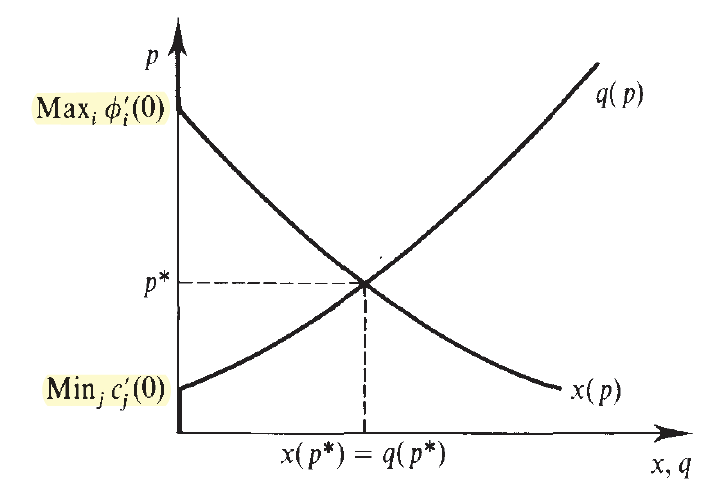
\includegraphics[width=0.5\linewidth]{figures/ASAD}
	 	\end{figure*}
	 	
	 	\begin{remark}
	 		The necessary condition for $((x^*_i), (y^*_j), p)$ to constitute a competitive equilibrium is 
	 		\begin{equation}
	 			p^* \in \left (
	 				\min_j c_j'(0),\ \max_i \phi_i'(0)
	 			\right )
	 		\end{equation}
	 	\end{remark}
	 	
	 	\begin{figure*}[h]
	 		\centering
	 		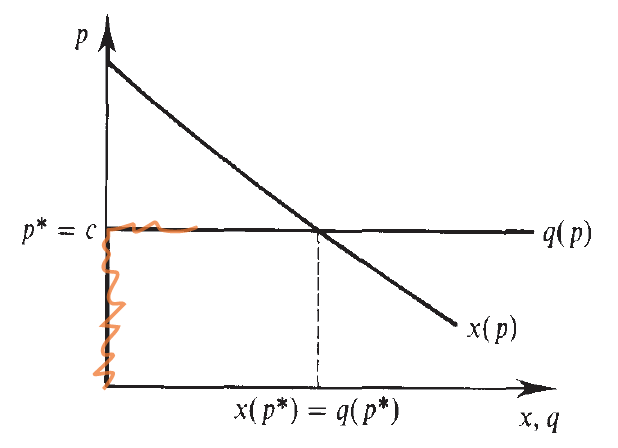
\includegraphics[width=0.5\linewidth]{figures/CSR}
	 		\caption{Constant Marginal Cost}
	 	\end{figure*}
	 	
	 	\paragraph{Comparative Statistics} Suppose each consumer's preferences are affected by a vector of exogenous parameters $\alpha \in \R^M$. And the technology is affected by exogenous parameters $\beta \in \R^S$. And the price faced by each consumer and each producer are affected by the tax/subsidy parameter $t \in \R^K$. Therefore,
	 	\begin{align}
	 		\phi_i(x_i, \alpha) \quad
	 		\hat{p}_i(p^*, t)\\
	 		c_j(q_j, \beta) \quad
	 		\hat{p}_j(p^*, t)
	 	\end{align}
	 	and the competitive equilibrium with interior solutions $((x^*_i), (y^*_j), p)$ and parameter set $\Theta = (\alpha, \beta, t)$ can be characterized by
	 	\begin{align}
	 		\phi_{i}^{\prime}\left(x_{i}^{*}, \alpha\right)&=\hat{p}_{i}\left(p^{*}, t\right) \quad i=1, \dots, I \\
	 		c_{j}^{\prime}\left(q_{j}^{*}, \beta\right)&=\hat{p}_{j}\left(p^{*}, t\right) \quad j=1, \ldots, J \\
	 		\sum_{i=1}^{I} x_{i}^{*}&=\sum_{j=1}^{J} q_{j}^{*}
	 	\end{align}
	 	
	 	\begin{remark}
	 		If all the relevant functions are differentiable, we can use the implicit function theorem to derive the marginal change in the equilibrium allocation and price in response to a differential change in the values of these parameters.
	 	\end{remark}
	 	
	 	\begin{example}[10.C.1 Comparative Statics Effects of a Sales Tax]
	 		Suppose there is a per-unit tax $t \geq 0$. As a result, consumers are facing $\hat{p}_i(p, t) = p + t$, and producers are facing $\hat{p}_j(p, t) = p$. Therefore, the equilibrium market price $p^*(t)$ as a function of $t$ must satisfy the market clearing condition:
	 		\begin{equation}
	 			x\left(p^{*}(t)+t\right)=q\left(p^{*}(t)\right)
	 		\end{equation}
	 		By the implicit function theorem,
	 		\begin{equation}
	 			p^{* \prime}(t)=-\frac{x^{\prime}\left(p^{*}(t)+t\right)}{x^{\prime}\left(p^{*}(t)+t\right)-q^{\prime}\left(p^{*}(t)\right)}
	 		\end{equation}
	 	\end{example}
	 	
	 \subsection{The Fundamental Welfare Theorems in a Partial Equilibrium Context}
	 	\begin{remark} Consider the two-good quasilinear economy, notice when consumer preferences are quasilinear, the boundary of the economy's utility possibility set is linear and all points in this boundary are associated with consumption allocations that differ only in the distribution of the numeraire among consumers. And the quasilinear form of the utility functions allows for an unlimited transfer of utility across consumers through transfers of the numeraire. Therefore, we only care about the total utility constraint, instead of individual utility constraint. Since if the total utility constraint is satisfies, we can re-distribute the numeraire among consumers to satisfy their individual utility constraint. For each levels of goods $\ell$ at $((\overline{x}_i, \overline{q}_j))	$, the attainable utility levels are
	 		\begin{equation}
	 			\left\{\left(u_{1}, \ldots, u_{I}\right) : \sum_{i=1}^{I} u_{i} \leq \sum_{i=1}^{I} \phi_{i}\left(\overline{x}_{i}\right)+\omega_{m}-\sum_{j=1}^{J} c_{j}\left(\overline{q}_{j}\right)\right\}
	 		\end{equation}
	 		which is a hyperplane with normal vector $(1, \cdots, 1)$. Thus, every Pareto optimal allocation must involve the quantities $((x_i^*), (q_j^*))$ that extend this boundary as far out as possible.
	 	\end{remark}
		
		\begin{definition}
			Equivalently, the social welfare optimization problem can be written as 
			\begin{align}
				\operatorname{max}_{\left(x_{1}, \ldots, x_{j}\right) \geq 0 \atop\left(q_{1}, \ldots, q_{j}\right) \geq 0}& \sum_{i=1}^{I} \phi_{i}\left(x_{i}\right)-\sum_{j=1}^{J} c_{j}\left(q_{j}\right)+\omega_{m} \\
				s.t.&\ \sum_{i=1}^{I} x_{i}-\sum_{j=1}^{J} q_{j}=0
			\end{align}
			The solution of the optimization problem is independent from $\omega_m$.
		\end{definition}
		
		\begin{definition}
			The term $\sum_{i} \phi_{i}\left(x_{i}\right)-\sum_{j} c_{j}\left(q_{j}\right)$ is known as the \textbf{(Marshallian) aggregate surplus}, which can be interpreted as \emph{the total utility generated from consumption of good less its costs of production (in terms of the numeraire).}
		\end{definition}
		
		\begin{proposition}[The First Fundamental Theorem of Welfare Economics]
			If the price $p^*$ and allocation $((x^*_i), (y^*_j), p)$ constitute a competitive equilibrium, then this allocation is Pareto optimal.
		\end{proposition}
		
		\begin{proof}[Idea of Proof]
			For above optimization, the corresponding Lagrangian is 
			\begin{equation}
				\mc{L} = \sum_{i=1}^{I} \phi_{i}\left(x_{i}\right)-\sum_{j=1}^{J} c_{j}\left(q_{j}\right)+\omega_{m} + \sum_i \alpha_i x_i + \sum_j \beta_j q_j + \mu \left (\sum_{j=1}^J q_j - \sum_{i=1}^I x_i \right)
			\end{equation}
			The necessary conditions gives
			\begin{align}
				\pd{\mc{L}}{x_i} &= \phi_i'(x_i) + \alpha_i - \mu = 0 \\
				\pd{\mc{L}}{q_j} &= -c_j'(q_j) + \beta_j + \mu = 0 \\
				&\sum_{j=1}^J q_j = \sum_{i=1}^I x_i
			\end{align}
			as well as the complementary slackness conditions, 
			\begin{align}
				\mu \leq c_{j}^{\prime}\left(q_{j}^{*}\right), \quad \text { with equality if } q_{j}^{*}>0 \quad j=1, \ldots, J \\
				\phi_{i}^{\prime}\left(x_{i}^{*}\right) \leq \mu, \quad \text { with equality if } x_{i}^{*}>0 \quad i=1, \ldots, I
			\end{align}
			By the envelope theorem, $\mu$ is the shadow price of relaxing the resource constraint, and it should be strictly positive at the optimal. Suppose we have a competitive equilibrium, by setting $\mu = p^*$, the competitive equilibrium becomes a Pareto optimal allocation.
		\end{proof}
		
		\begin{remark}
			The first fundamental theorem is a formal expression of Adam Smith's invisible hand and is a result that holds with considerable generality.
		\end{remark}
		
		\begin{remark}
			A crucial assumption for the first fundamental theorem is \emph{markets are complete}, in the sense that there is a market for every relevant commodity and all market participants act as price takers.
		\end{remark}
		
		\begin{proposition}[The Second Fundamental Theorem of Welfare Economics]
			For any Pareto optimal levels of utility $(u^*_i)$, there are transfers of the numeraire commodity $(T_i)$ satisfying $\sum_i T_i = 0$, such that a competitive equilibrium reached from the endowments $(\omega_{mi}+T_i)$ yields $(u_i^*)$.
		\end{proposition}
		
		\begin{remark}
			A crucial assumption for the second fundamental theorem (but not required by the first one) is the \ul{convexity of preferences and production sets}.
		\end{remark}
		
		\begin{remark}
			The competitive price is exactly equal to the shadow price on the resource constraint for good in the Pareto optimality problem. Hence, \emph{A good's price in a competitive equilibrium reflects precisely its marginal social value. In a competitive equilibrium, each firm, by operating at a point where price equals marginal cost, equates its marginal production cost to the marginal social value of its output. Similarly, each consumer, by consuming up to the point where marginal utility from a good equals its price, is at a point where the marginal benefit from consumption of the good exactly equals its marginal cost.}
		\end{remark}
		
		\subsection{Welfare Analysis in the Partial Equilibrium Model}
		
		\begin{definition}
			A \textbf{social welfare function} $W(u_1, \dots, u_I)$ assigning a social welfare value to every utility vector $(u_i)$.
		\end{definition}
		
		\begin{proposition}
			Suppose there is some central authority who redistributes wealth by means of transfers of the numeraire commodity in order to maximize social welfare. \ul{Given quasilinear preferences for individuals}, the changes in social welfare can be measured by changes in the Marshallian aggregate surplus for \ul{any social welfare function} that society may have.
		\end{proposition}
		
		\begin{proof}[Justify]
			As argued before, the utility possible set \ul{given consumption and production set} can be written as 
			\begin{equation}
				\mc{U} := \left\{\left(u_{1}, \ldots, u_{I}\right) : \sum_{i=1}^{I} u_{i} \leq \omega_{m}+
				\underbrace{\sum_{i=1}^{I} \phi_{i}\left(x_{i}\right)-\sum_{j=1}^{J} c_{j}\left(q_{j}\right)}_{S(x_1, \cdots, x_I, q_1, \cdots, q_J)}
				\right\}
			\end{equation}
			and the central authority is maximizing $W((u_i))$ given $(u_i) \in \mc{U}$. Given $\pd{W}{u_i} \geq 0$ with at least one $\pd{W}{u_i} > 0$, the increase of aggregate surplus relaxes the constraint set, and rise the maximal of $W$.
		\end{proof}
		
		\begin{figure*}[h]
			\centering
			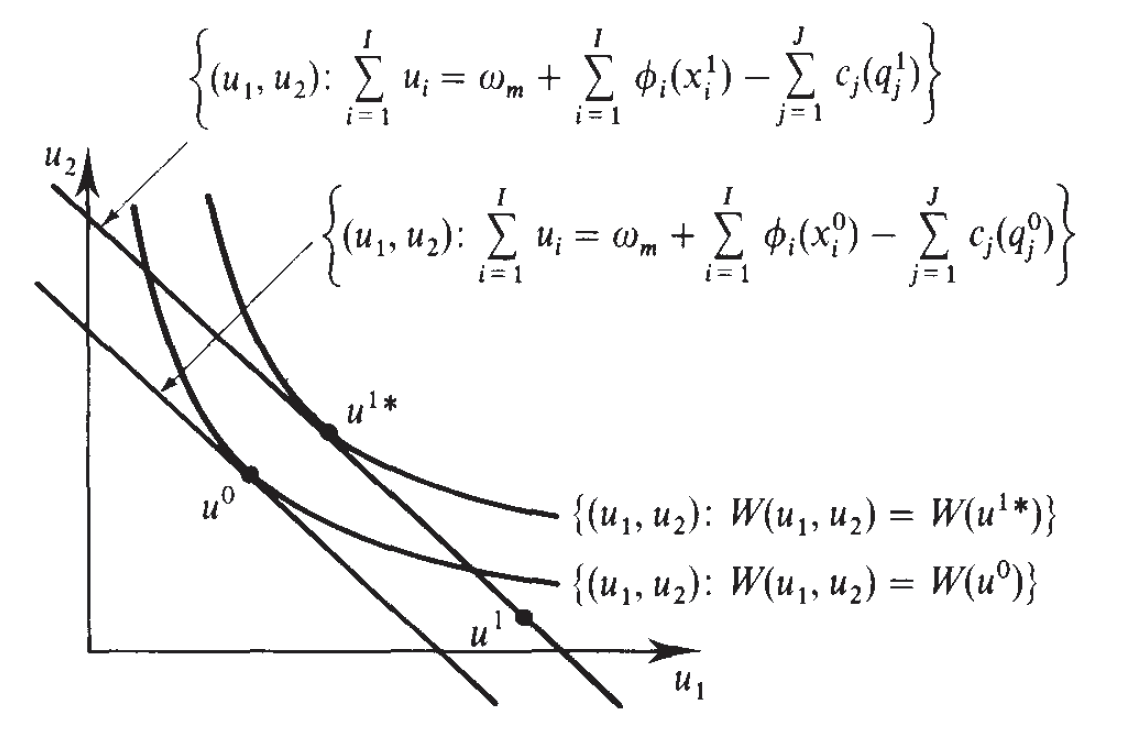
\includegraphics[width=0.5\linewidth]{figures/welfare1}
		\end{figure*}
		
		\begin{remark}
			Thus, as long as redistribution of wealth is occurring to maximize a social welfare function, changes in welfare can be measured by changes in Marshallian aggregate surplus (for any social welfare function).
		\end{remark}
		
		\begin{proposition}[Geometrical Interpretation of Surplus]
			Consider a differential change $((dx_i), (dq_j))$ in quantities of good $\ell$ such that $\sum_i dx_i = \sum_j dq_j$ (market clears). Define $dx := \sum_i dx_i$ and $dq := \sum_j dq_j$. Then the total derivative of $S$ is 
			\begin{align}
				dS &= \sum_{I=1}^I \phi'_i(x_i) dx_i - \sum_{j=1}^J c'_j(q_j) dq_j \\
				&= P_i(x) \sum_{I=1}^I dx_i - C'(q) \sum_{j=1}^J dq_j \\
				&= [P(x) - C'(x)] dx \\
				&\implies S(x) = S(0) + \int_0^x [P(z) - C'(z)]dz
			\end{align}
		\end{proposition}
		
		\begin{figure*}[h]
			\centering
			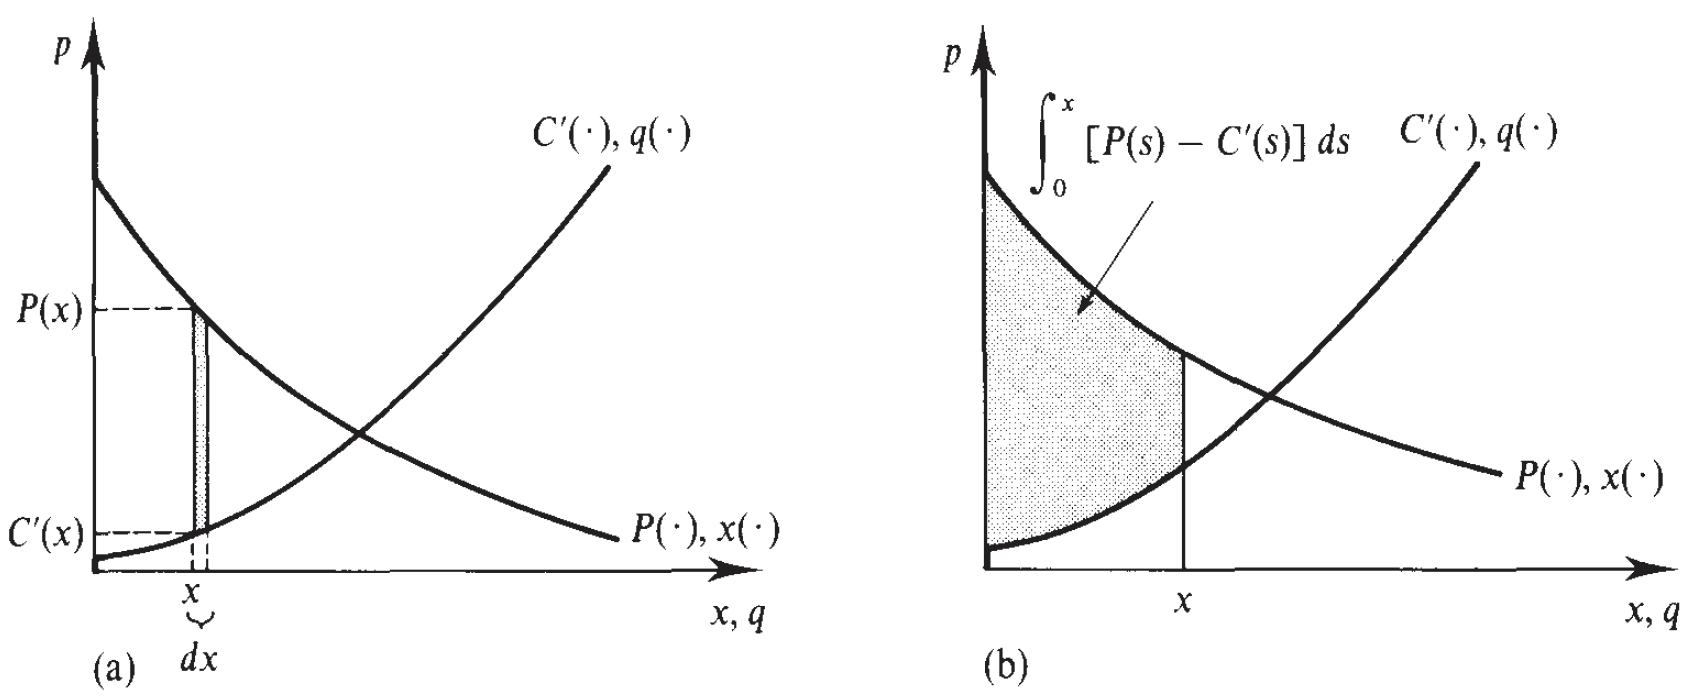
\includegraphics[width=0.5\linewidth]{figures/agg_surplus}
		\end{figure*}
		
		\begin{example}[The Welfare Effects of a Distortionary Tax]
			
		\end{example}
		
		\subsection{Free-Entry and Long-Run Competitive Equilibria}
		\begin{assumption}
			Suppose there is an infinite number of potential firms has access to a technology of production good $\ell$ with cost function $c(q)$, where $q$ is the \emph{individual} firm's output for good $\ell$. Further, assume $c(0) = 0$ so that firm can earn zero profits by operation at $q=0$.
		\end{assumption}
		
		\begin{assumption}
			Suppose there are $J$ identical firms active in the industry, and all active firms produce the same output level.
		\end{assumption}
		
		\begin{proposition}
			If all firms, active and potential, take prices as unaffected by their own actions, this implies that \ul{active firms must earn exactly zero profits} in any long-run competitive equilibrium; \emph{otherwise, we would have either no firms willing to be active in the market (if profits were negative) or an infinite number of firms entering the market (if profits were positive).}
		\end{proposition}
		
		\begin{definition}[10.F.1]
			Given aggregate demand function $x(p)$ and cost function $c(q)$ with $c(0) = 0$, a triple $(p^*, q^*, J^*)$ is a \textbf{long-run competitive equilibrium} if
			\begin{enumerate}[(i)]
				\item $q^*$ solves $\max_{q \geq 0} p^* q - c(q)$ (profit maximization);
				\item $x(p^*) = J^* q^*$ (market clears);
				\item $p^* q^* - c(q^*) = 0$ (zero profit free entry condition).
			\end{enumerate}
		\end{definition}
		
		\begin{definition}
			Given cost and profit functions $c(\cdot)$ and $\pi(\cdot)$, the \textbf{long-run aggregate supply correspondence} is defined
			\begin{equation}
				Q(p) = \begin{cases}
					\infty &\tx{ if } \pi(p) > 0 \\
					\left\{
						Q \geq 0: Q = Jq,\ J \in \Z,\ q \in q(p)
					\right\} &\tx{ if } \pi(p) = 0
				\end{cases}
			\end{equation}
		\end{definition}
		
		\begin{proposition}
			$p^*$ is a long-run competitive equilibrium price \ul{if and only if} $x(p^*) \in Q(p^*)$.
		\end{proposition}
		
		\begin{example}[Constant marginal cost]
			\begin{align}
				p^* &= \overline{c} \\
				\overline{q} &= \argmin \frac{c(q)}{q} \\
				\frac{c(\overline{q})}{(\overline{q})} &= \overline{c} \\
				Q(p) &= \begin{cases}
					\infty &\tx{ if } p > \overline{c} \\
					\left\{Q \geq 0: Q = J \overline{q},\ J \in \Z \right\} &\tx{ if } p = \overline{c} \\
					0 &\tx{ if } p < \overline{c}
				\end{cases}
			\end{align}
		\end{example}
		
		\begin{example}[Short-Run and Long-Run Comparative Statistics]
			Consider a long-run equilibrium with $J^*$ active firms each producing $q^*$ units of output. Suppose there is some shock to demand. Firms face a short run cost function $c_s(\cdot)$ that differs from the long-run cost function $c(\cdot)$ because the input fixation. For example the long run cost function is 
			\begin{equation}
				c(q)=\left\{\begin{array}{ll}{K+\psi(q)} & {\text { if } q>0} \\ {0} & {\text { if } q=0}\end{array}\right.
			\end{equation}
			with $\psi(0) = 0$, $\psi'(q), \psi''(q) > 0$. And the short run cost function is 
			\begin{equation}
				c_{s}(q)=K+\psi(q) \quad \text { for all } q \geq 0
			\end{equation}
			\ul{In the short run}, the $J^*$ firms optimize according to $c_s(\cdot)$, and \ul{in the long run}, the profit maximization is solved using $c(\cdot)$.
		\end{example}
		
		\begin{figure*}[h]
			\centering
			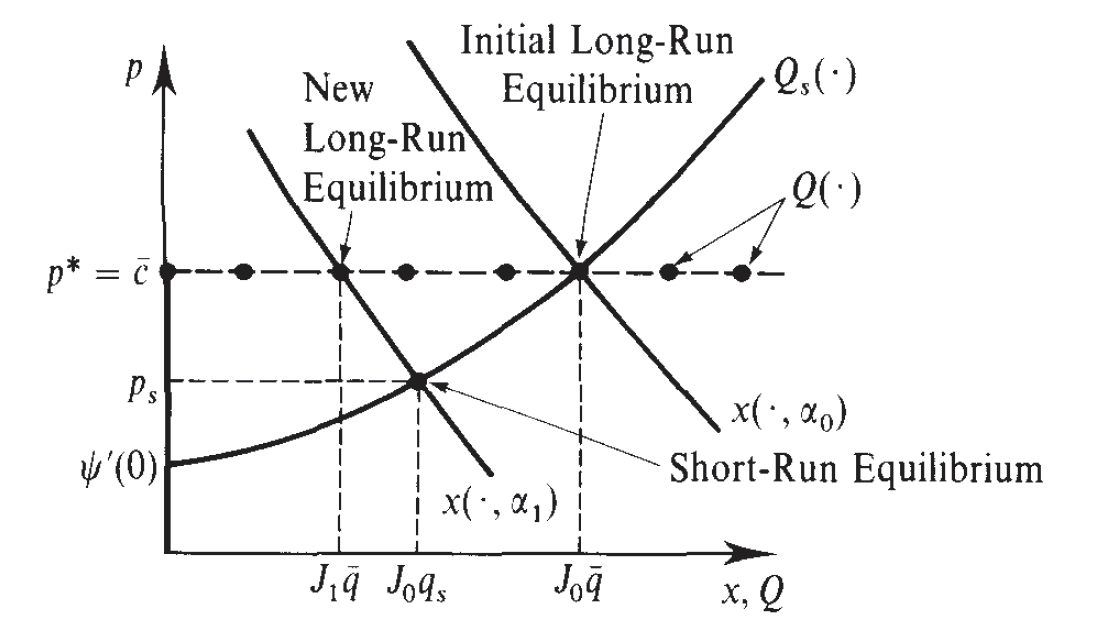
\includegraphics[width=0.5\linewidth]{figures/SRLR_CS}
			\caption{Short-Run and Long-Run Comparative Statics with Lumpy Fixed Costs that Are Sunk in the Short Run}
		\end{figure*}
		
		\begin{remark}
			In previous analysis, we proposed there are only two types of time span. It may often be reasonable to think that there are several distinct short-run stages corresponding to different levels of adjustment costs associated with different decisions: in the very short run, production may be completely fixed; in the medium run, some inputs may be adjusted while others may not be; perhaps entry and exit take place only in the "very long run."
		\end{remark}
		
		\begin{remark}
			In the previous analysis, we assumed the isolation between the short-run and long-run, however, there may exists the probability of inter-temporal substitution by consumers.
		\end{remark}
	
	\section{Chapter 13. Adverse Selection, Signalling, and Screen}
		\subsection{Informational Asymmetries and Adverse Selection}
		\begin{definition}
			\textbf{Adverse selection} is said to occur when an informed individual's trading decision depends on her \ul{unobservable characteristics} in a manner that \ul{adversely affects} the uninformed agents in the market.
		\end{definition}
		
		\subsubsection{Economy Setup}
		
		\paragraph{Firm} Firms are identical with constant return to scale production function $f$ using only labor as input factor. Further, assuming the price of product is 1, that is, the firm is producing numeraire good. Firms are risk-neutral and maximizing the expected profit.
		
		\paragraph{Worker} Suppose there are $N$ workers, each with productivity $\theta \in [\underline{\theta}, \overline{\theta}] \subset \R$. The distribution of productivity $\theta$ follows distribution $F(\theta)$. Each worker earns $r(\theta)$ on her own through home production. Therefore, a worker will accept a job offer if and only if $w \geq r(\theta)$ (we assume that she accepts if she is indifferent).
		
		\begin{assumption}
			Assume the distribution of productivity, $F(\theta)$, is non-degenerate, that is, there exists at least two distinct types of workers.
		\end{assumption}
		
		\subsubsection{Equilibrium with Symmetric Information}
		\par If the productivity $\theta$ for each worker is \ul{publicly observable}, then each different type of worker is a distinct good, there is a distinct equilibrium wage $w^*(\theta)$ \ul{for each type $\theta$}. Given the competitive, constant returns nature of the firms, in a competitive equilibrium we have $w^*(\theta) = \theta$ for all $\theta$, and the set of workers accepting employment in a firm is $\{\theta: r(\theta) \leq \theta \}$. Such equilibrium outcome is Pareto optimal by the first fundamental theorem of welfare economics. Let $\id{\theta}$ denote the worker of type $\theta$ being employed by a firm, then the aggregate surplus is
		\begin{equation}
			Surplus = \int_{\underline{\theta}}^{\overline{\theta}} N \left [
				\id{\theta} \theta + (1-\id{\theta})r(\theta)
			\right ] dF(\theta)
		\end{equation}
		And the surplus is maximized when one worker is employed if and only if $r(\theta) \leq \theta$.
		
		\begin{remark}
			When workers' types are not observable, the wage rate must be independent of a worker's type, and so we will have a single wage rate $w$ for all workers.
		\end{remark}
		
		\paragraph{Labor Supply} Given a wage rate $w$, a worker with productivity $\theta$ would accept the offer if and only if $r(\theta) \leq w$. Therefore, the set of types of workers employed would be 
		\begin{equation}
			\Theta(w) = \{\theta: r(\theta) \leq w\}
		\end{equation}
		
		\paragraph{Labor Demand} Given a wage rate $w$, let $\mu$ denote the expected(average) productivity of people whole get employed, the demand for labor is given by 
		\begin{equation}
			z(w) = \begin{cases}
				0 &\tx{ if } \mu < w \\
				[0, \infty] &{ if } \mu = w \\
				\infty &\tx{ if } \mu > w
			\end{cases}
		\end{equation}
		
		\paragraph{Equilibrium} When the set of workers, $\Theta^*$, is get employed, then $\mu = \expect{\theta|\theta \in \Theta^*}$. For the demand of labor to be non-zero and finite, the wage rate supporting an equilibrium outcome can only be $w^* = \mu = \expect{\theta|\theta \in \Theta^*}$.
		
		\begin{definition}
			In a competitive labor market with unobservable worker productivity levels, a \textbf{competitive equilibrium} consists of a wage rate $w^*$ and a set $\Theta^*$ of worker types who accept employment such that
			\begin{equation}
				\Theta^* = \{\theta: r(\theta) \leq w^*\}
			\end{equation}
			and 
			\begin{equation}
				w^* = \expect{\theta|\theta \in \Theta^*}
			\end{equation}
		\end{definition}
		
		\begin{remark}
			The definition of competitive equilibrium involves rational expectation of firms. However, the expectation is not well-defined when $\Theta^* = \varnothing$. Conventionally, we use the unconditional expectation in the definition of a equilibrium, $w^* = \expect{\theta}$, whenever nobody is employed.
		\end{remark}
		
		\subsubsection{Equilibria with Asymmetric Information and Pareto Inefficiency}
		\begin{example}
			Consider the case when $r(\theta) = r$ for all $\theta$, and suppose $F(r) \in (0, 1)$. That's, all workers have the same at-home earning but different productivity at work. The Pareto optimal outcome requires a worker to be employed if and only if $\theta \geq r$. For any given wage rate $w^*$, the equilibrium employment would be either $[\underline{\theta}, \overline{\theta}]$ (if $w^* \geq r$) or $\varnothing$ (if $w^* < r$). Further, the competitive equilibrium wage rate $w^*$ must satisfy $w^* = \expect{\theta|\theta \in \Theta^*}$. In either case, $w^* = \expect{\theta}$. The Pareto optimal outcome will never be attained.\\
			\emph{Interpretation: if there is a high fraction of low-productivity workers then, because firms cannot distinguish good workers from bad, they will be unwilling to hire any workers at a wage rate that is sufficient to have them accept employment (i.e., a wage of at least $r$). On the other hand, if there are very few low-productivity workers, then the average productivity of the workforce will be above $r$, and so the firms will be willing to hire workers at a wage that they are willing to accept.}
		\end{example}
		
		\subsubsection{Adverse Selection and Market Unraveling}
		\begin{figure*}[h]
			\centering
			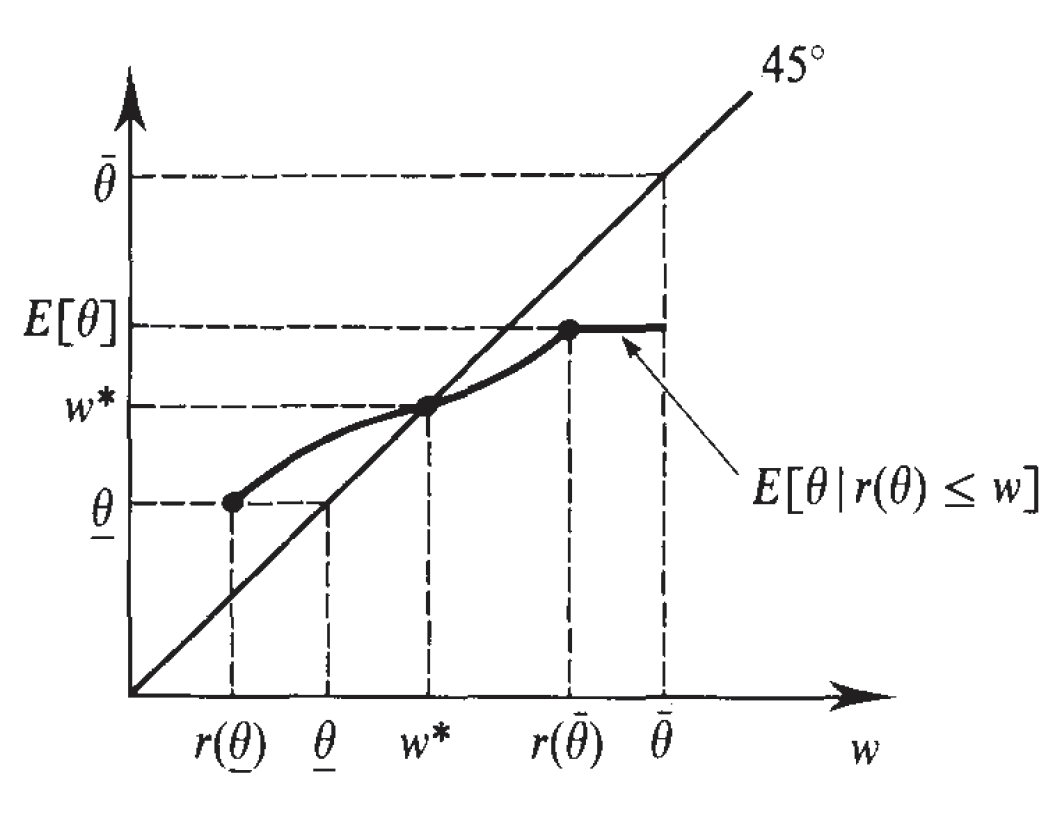
\includegraphics[width=0.4\linewidth]{figures/adverse_selection}
			\caption{Adverse Selection Competitive Equilibrium}
		\end{figure*}		

		\begin{example}[Adverse Selection]
			Suppose $r(\theta) \leq \theta$ for all $\theta$, and $r(\cdot)$ is strictly increasing. Further, assume the density function $f(\theta) > 0$ for every $\theta \in [\underline{\theta}, \overline{\theta}]$. The Pareto optimal requires every worker to be employed. However, this generates adverse selection: because the payoff of home production is greater for more capable workers, only less capable workers  accept employment at any given wage rate $w$. In this setup, the equilibrium attained would be one in which only workers with productivity $\underline{\theta}$ employed. At the competitive equilibrium, the wage rate must satisfy
			\begin{equation}
				w^* = \expect{\theta|\theta \in \Theta^*} \equiv \expect{\theta|r(\theta) \leq w^*}
			\end{equation}
			Note that $\expect{\theta|r(\theta) \leq w^*}$ is increasing in $w^*$ for $w^* \in [r(\underline{\theta}), r(\overline{\theta})]$.
			Further, note that for workers with productivity $\overline{\theta}$ to get employed, $w^*$ must satisfy $w^* \geq r(\overline{\theta})$. However, the firm cannot break even because $\expect{\theta} < r(\overline{\theta})$. After the best workers are driven out of the market, the average productivity falls and the second best workers are driven out of the market as well. Lastly, only workers with $\underline{\theta}$ are employed.
		\end{example}
		
		\begin{figure*}[h]
			\centering
			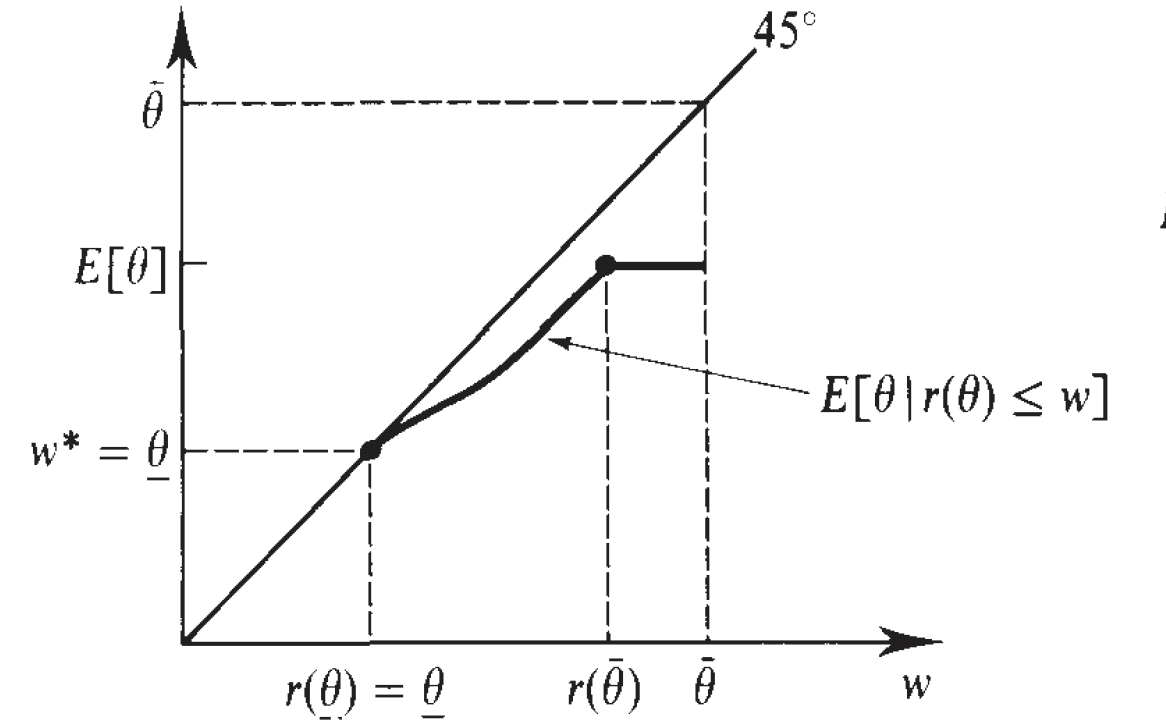
\includegraphics[width=0.5\linewidth]{figures/complete_market_failure}
			\caption{Complete Market Failure}
		\end{figure*}
		
		\begin{remark}[Multiple Equilibra]
			Multiple competitive equilibria can arise because there is virtually no restriction on the slope of the function $\expect{\theta|r(\theta) \leq w}$. At any wage $w$, this slope depends on the density of workers who are just indifferent about accepting employment and so it can vary greatly if the density varies. Multiple equilibria can be \textbf{Pareto ranked}. Firms earn zero profits in all equilibria, and workers are better off if the wage rate is higher. Thus the equilibrium with the highest wage \textbf{Pareto dominates} all the others.
		\end{remark}
		
		\begin{figure*}[h]
			\centering
			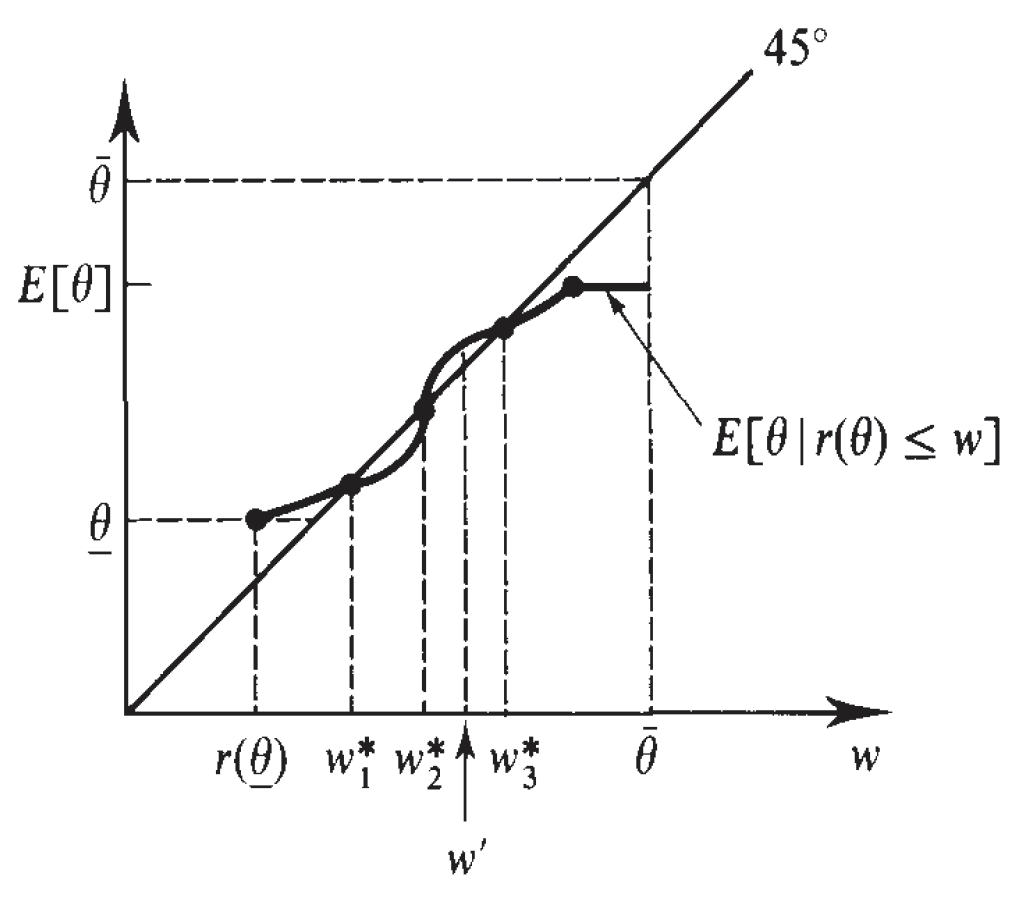
\includegraphics[width=0.4\linewidth]{figures/multiple_competitive_eq.png}
			\caption{Multiple Competitive Equilibra}
		\end{figure*}
		
		\begin{definition}
			\textbf{Coordinate failure} occurs when the wage is too low because firms expect that the productivity of workers accepting employment is poor and, at the same time, only bad workers accept employment precisely because the wage is low. Therefore, those low-wage equilibria are resulted from coordinate failures.
		\end{definition}
	
	\chapter{General Equilibrium Analysis}
	\section{Chapter 15. General Equilibrium Theory: Some Examples}
		\subsection{Pure Exchange: The Edgeworth Box}
		\subsubsection{Model Setup}
		\begin{definition}
			A \textbf{pure exchange economy} is an economy in which there are no production opportunities.
		\end{definition}
		
		\paragraph{Consumers} act as price takers. Each consumer $I$ possesses a preference $\pref_i$ over consumption set $X_i$, a consumption vector $x_i \equiv (x_{\ell I})_\ell \in \R^L_+$, and initial \textbf{endowment vector} $\omega_i \equiv (\omega_{\ell I})_\ell)$. The total endowment of good $\ell$ is therefore $\overline{\omega}_\ell = \sum_i \omega_{\ell I}$.
		\begin{definition}
			An \textbf{allocation} can be characterized as a list of consumption vectors
			\begin{equation}
				\mc{A} := (x_i)_i = ((x_{\ell I})_\ell)_i
			\end{equation}
			An allocation is said to be \textbf{feasible} if 
			\begin{equation}
				\forall \ell,\ \sum_{I=1}^I x_{\ell I} \leq \sum_{I=1}^I \omega_{\ell I}
			\end{equation}
			when the equality holds, $\mc{A}$ is said to be \textbf{nonwasteful}.
		\end{definition}
		
		\subsubsection{Consumers' Behaviour}
		\paragraph{} When $I=L=2$, any nonwasteful and feasible allocation can be represented as a vector inside the Edgeworth box. Given an exogenous price vector $p \in \R^2$, the budget set of consumer $I$ can be written as 
		\begin{equation}
			B_i (p) = \{
				x_i \in \R^2_+: p \cdot x_i \leq p \cdot \omega_i
			\}
		\end{equation}
		Therefore consumers' budget sets are separated by a hyperplane with norm $p$ (the budget line), and only allocations on the budget line are affordable to both consumer simultaneously at given price $p$.
		
		\begin{figure*}[h]
			\centering
			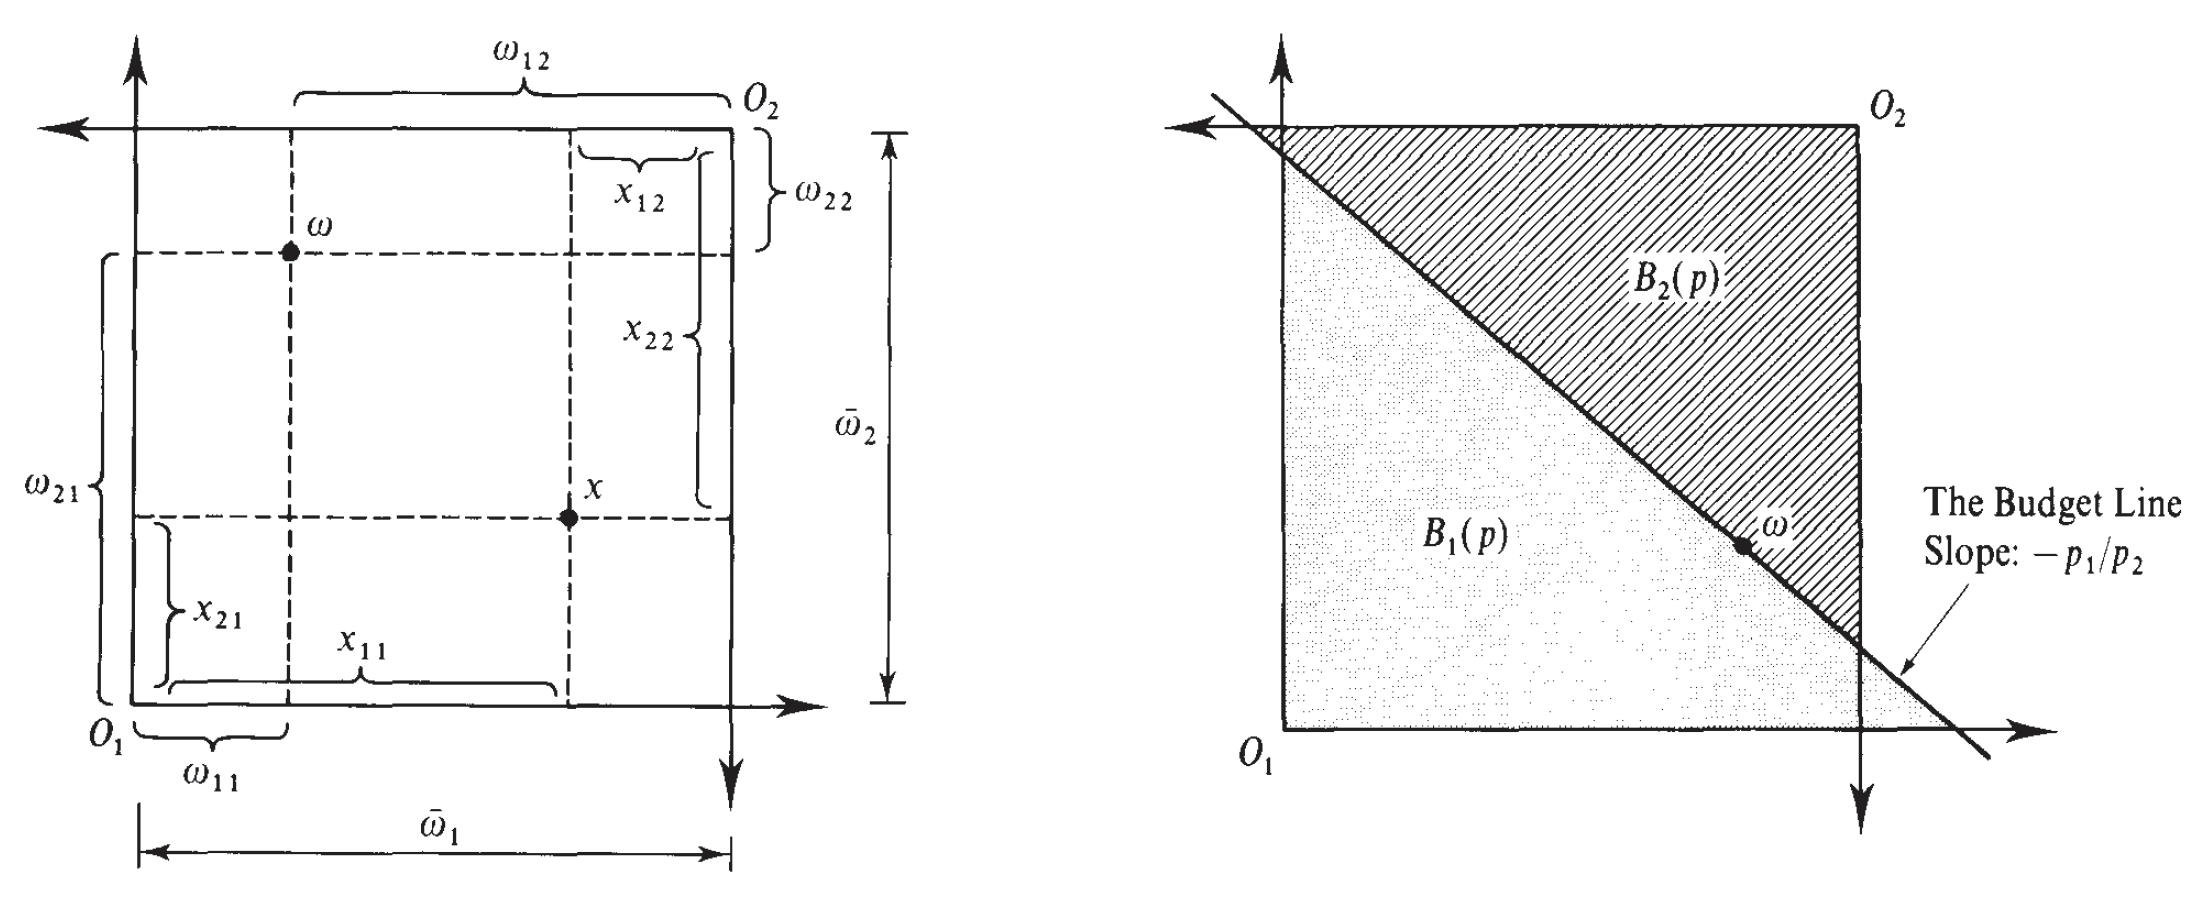
\includegraphics[width=0.8\linewidth]{figures/EWBox_Budget.png}
			\caption{Edgeworth Box and Budget Set}
		\end{figure*}	
		
		\begin{assumption}
			Except where otherwise noted, we assume that $\pref_i$ is strictly convex, continuous, and strongly monotone.
		\end{assumption}
		
		\paragraph{} Given an exogenous price vector $p$ and assumptions on consumes' preference, denote consumer $I$'s demand \emph{function} as $x_i(p, p\cdot \omega_i)$.
		
		\begin{definition}
			The \textbf{offer curve} is defined to be the trace of values of consumer $i$'s demand function while $p$ is changing.
			\begin{equation}
				OC_i := \left \{
				x \in \R^2_+:
				\exists p \in \R^2_{++}\ s.t.\ x = x_i(p, p\cdot \omega_i)
				\right \} \subset \tx{Edgeworth Box}
			\end{equation}
		\end{definition}
		
		\begin{remark}
			The offer curve passes through the endowment point $\omega_i$. In particular, consumer chooses not to exchange when the relative price equals MRS at the initial endowment.
		\end{remark}
		
		\begin{remark}
			Since $\omega$ is always attainable, therefore, the consumer's offer curve lies entirely within the upper contour set of $\omega_i$. As a result, if indifference curves are smooth, the offer curve must be tangent to the consumer's indifferent curve at the endowment.
		\end{remark}
		
		\begin{figure*}[h]
			\centering
			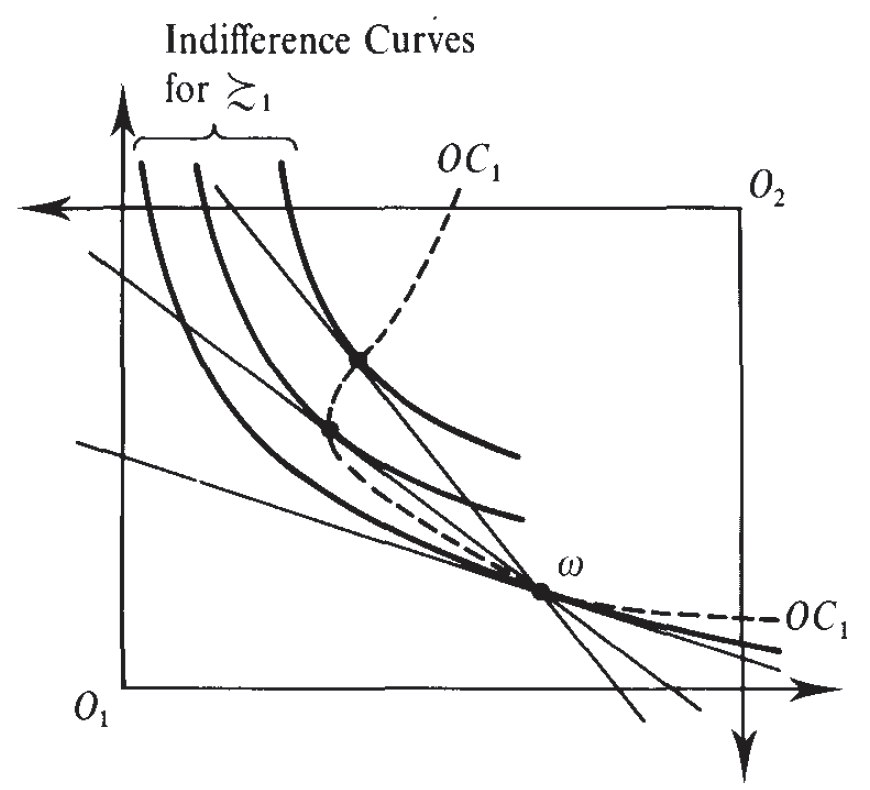
\includegraphics[width=0.35\linewidth]{figures/OC.png}
			\caption{Offer Curve of Consumer 1}
		\end{figure*}
		
		\begin{definition}
			Consumer $i$ is called a \textbf{net demander} for commodity $\ell$ when $x_{\ell i}(p, \omega_i \cdot p) > \omega_{\ell i}$, and a \textbf{net supplier} if $x_{\ell i}(p, \omega_i \cdot p) < \omega_{\ell i}$.
		\end{definition}
		
		\begin{figure*}[h]
			\centering
			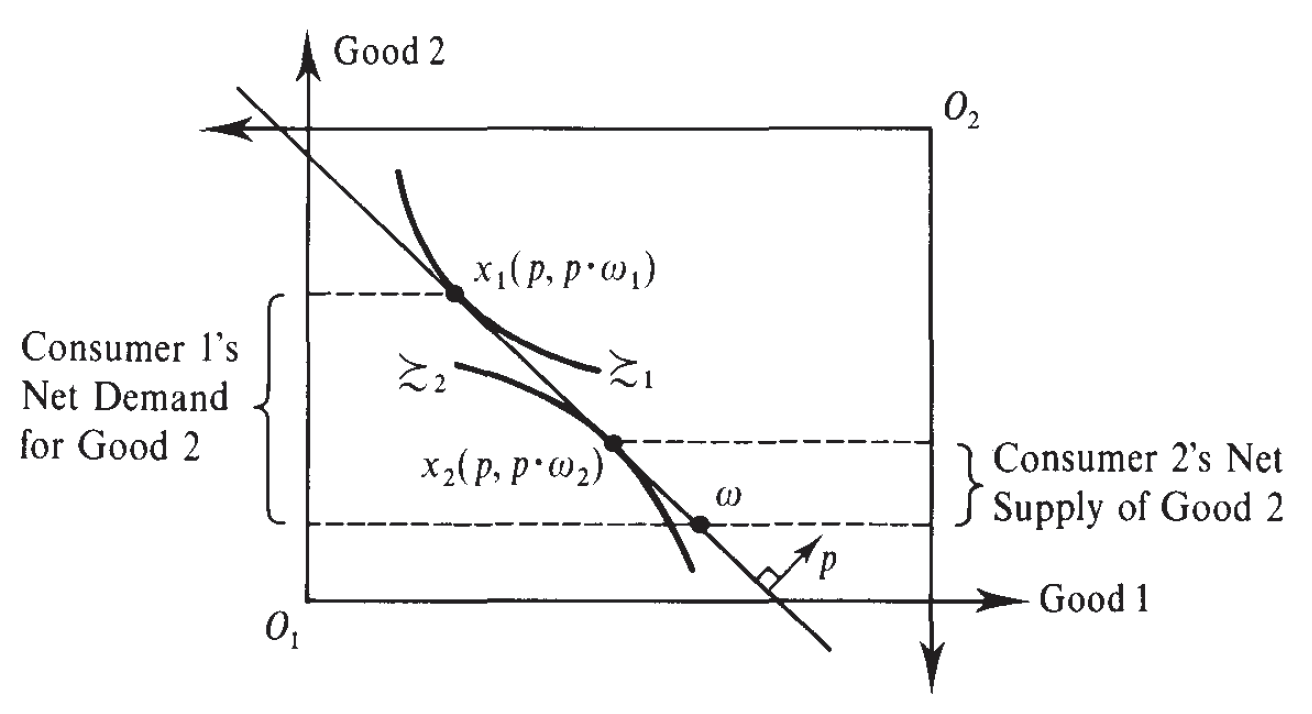
\includegraphics[width=0.5\linewidth]{figures/net_supplier}
			\caption{An Incompatible Price Vector}
		\end{figure*}
		
		\begin{definition}[15.B.1]
			A \textbf{Walrasian/Competitive Equilibrium} for an Edgeworth Box economy is a price-allocation tuple $((x^*_i)_i, p^*)$ in the Edgeworth box(markets cleared) such that
			\begin{equation}
				\forall i \in \{1,2\},\ x_i^* \pref_i x_i'\ \forall x_i' \in B_i(p^*)
			\end{equation}
		\end{definition}
		
		\begin{proposition}
			Any intersection of the consumers' offer curves at an allocation different $\omega$ corresponds to an equilibrium because any intersection $x^*$ is the optimal consumption bundle for each consumer for the budget line goes through $\omega$ and $x^*$.
		\end{proposition}
		
		\begin{proof}
			To justify the equilibrium, firstly notice that every point in the Edgeworth box clears the markets. Secondly, for consumer 1, suppose $x^*_1$ is the demand when price vector $p'$ is given. If the budget line given by $p'$ is less steeper than line between $x^*$ and $\omega$, $x^*_i$ becomes non-affordable. If the budget line resulted from $p'$ is more steeper, there exists $x' \neq x^*$ lies in the intersection of the upper contour set of $x^*$ and budget set for consumer 1, this contradicts the fact that $x^*$ is the demand. Therefore $x^*_1$ is the demand when price vector $(x^* - \omega)$ is given.
			With a similarly argument for the other consumer, we conclude at $x^*$, both consumer are optimizing with respect to the price given by budget line $x^*$ to $\omega$.
		\end{proof}
		
		\begin{remark}
			If $p^*$ is a Walrasian equilibrium price, then for any $\alpha > 0$, the price vector $\alpha p^*$ is also an equilibrium price. Therefore, the equilibrium is fully determined by the \ul{relative prices}.
		\end{remark}
		
		\begin{remark}
			It is possible for multiple equilibria to exist.
		\end{remark}
		
		\begin{figure*}[h]
			\centering
			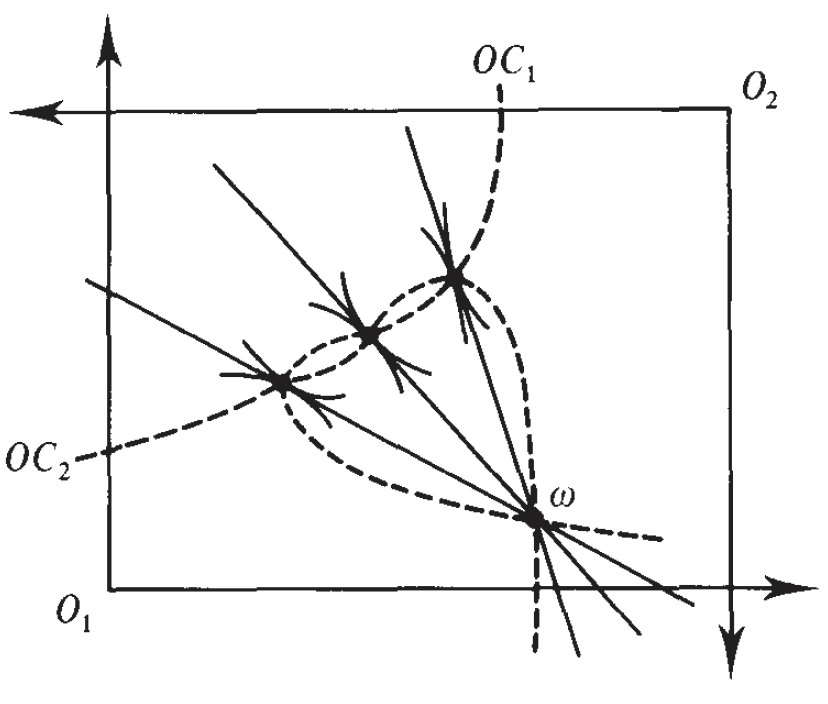
\includegraphics[width=0.3\linewidth]{figures/multiple_eq}
			\caption{Multiple Equilibria}
		\end{figure*}
		
		\begin{remark}
			It is also possible that no equilibrium exists.
		\end{remark}
		
		\begin{figure*}[h]
			\centering
			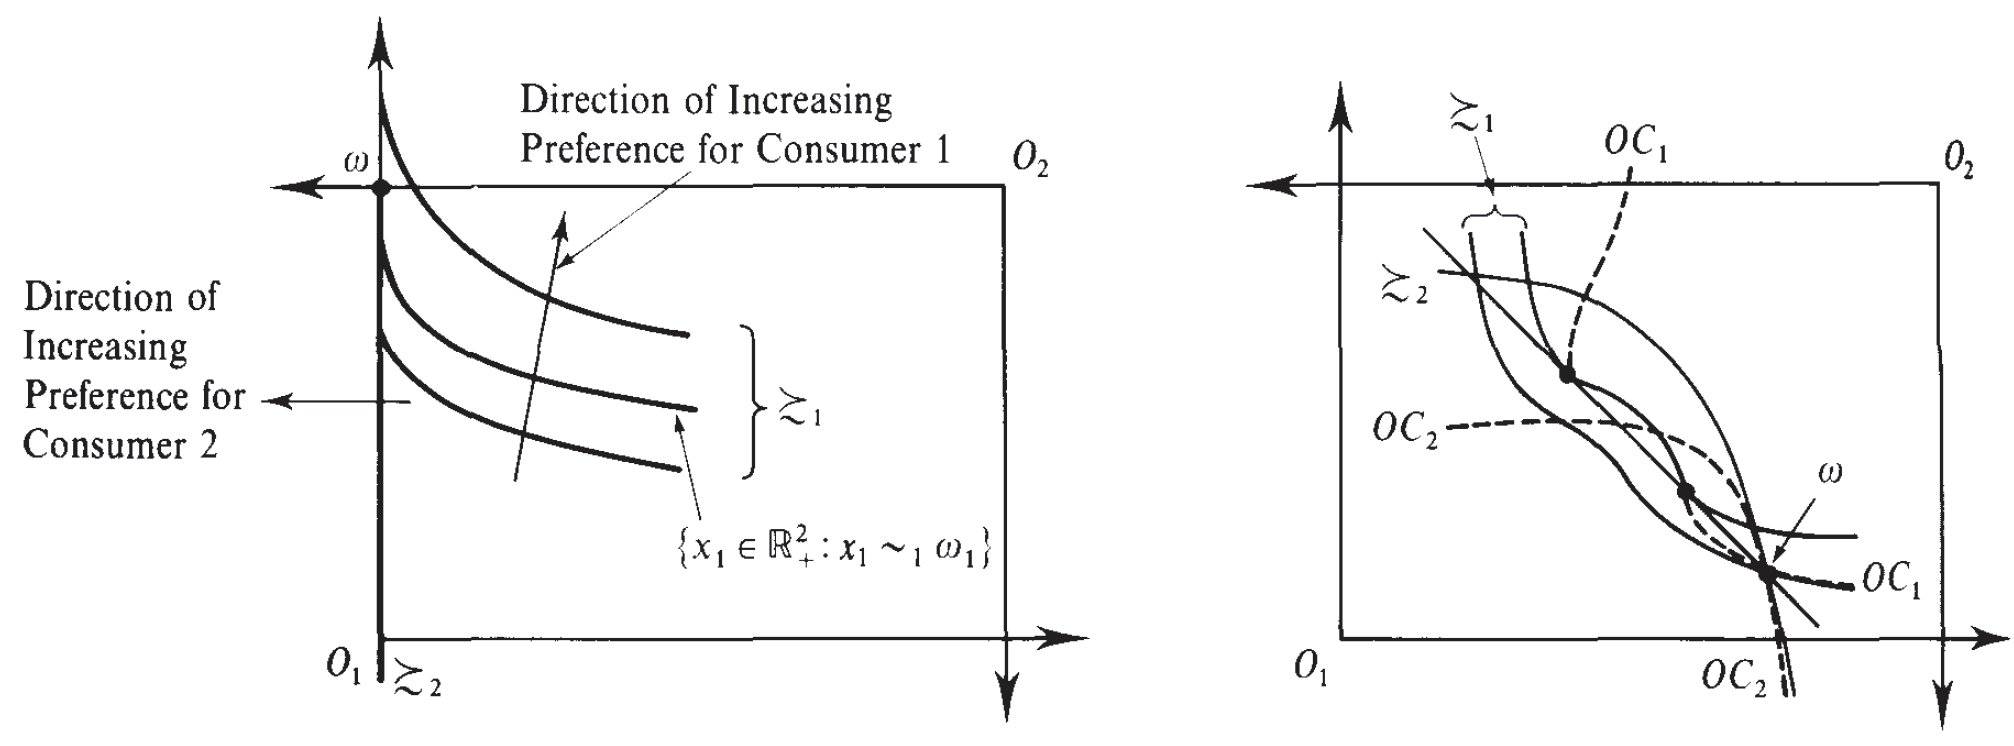
\includegraphics[width=0.8\linewidth]{figures/none_eq.png}
			\caption{No Equilibrium}
		\end{figure*}
		
		\subsubsection{Welfare}
		\begin{definition}[15.B.2]
			An allocation $x$ in the Edgeworth box is \textbf{Pareto optimal/efficient} if there is no other allocation $x'$ in the Edgeworth box such that $x_i' \pref_i x_i\ \forall i$ and $x_i' \succ_i x_i$ for some $i$.
		\end{definition}
		
		\begin{remark}
			if a Pareto optimal allocation x is an interior point of the Edgeworth box, then the consumers' indifference curves through $x$ must be tangent (assuming that they are smooth).
		\end{remark}
		
		\begin{definition}
			The \textbf{Pareto set} is defined to be the set of all Pareto optimal allocations. The \textbf{contract curve} is a subset of the Pareto set on which both consumers do at least as well as at $\omega$.
		\end{definition}
		
		\begin{figure*}[h]
			\centering
			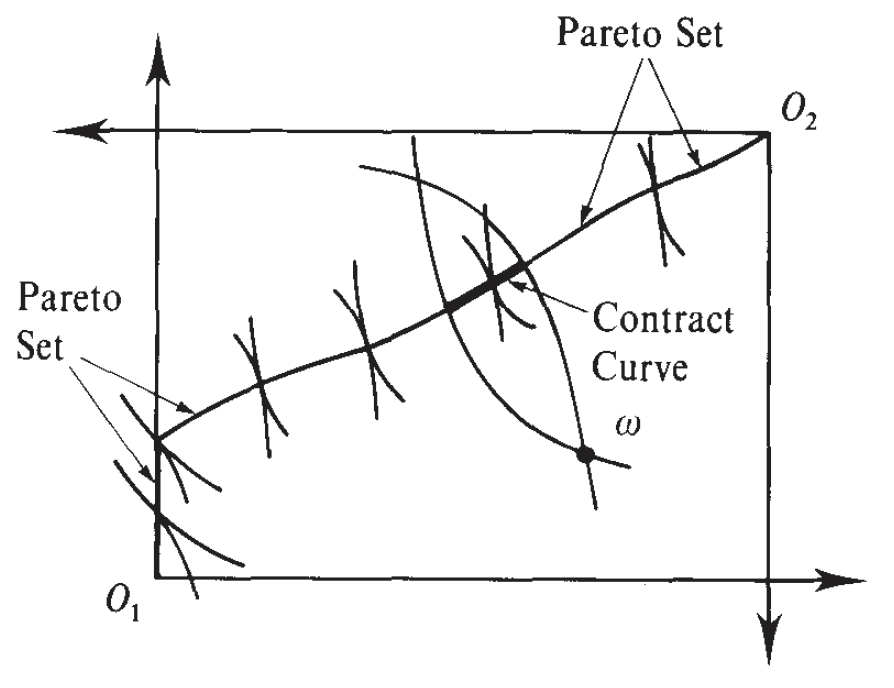
\includegraphics[width=0.4\linewidth]{figures/Pareto_contract}
			\caption{The Pareto Set and the Contract Curve}
		\end{figure*}
		
		\begin{remark}
			These allocations in the contract curve are the only points at which both of them do as well as at their initial endowments and for which there is no alternative trade that can make both consumers better off.
		\end{remark}
		
		\begin{proposition}[The First Fundamental Theorem of Welfare Economics]
			Any Walrasian equilibrium allocation $x^*$ belongs to the Pareto set.
		\end{proposition}
		
		\begin{proposition}
			Any Walrasian equilibrium lies in the contract curve, otherwise consumers can always consumer $\omega_i$ instead and this would contradicts the definition of Walrasian equilibrium.
		\end{proposition}
		
		\begin{definition}
			An allocation $x^*$ in the Edgeworth box is \textbf{supportable as an equilibrium with transfers} if there exists $(p^*, (T_i))$ satisfying $\sum_i T_i = 0$, such that for all consumer $i$
			\begin{equation}
				x_i^* \pref_i x_i' \ \forall x_i' \in \mc{B}(p^*, p^*\cdot \omega_i + T_i)
			\end{equation}
		\end{definition}
		
		\begin{proposition}[The Second Fundamental Theorem of Welfare Economics]
			If the preferences of the two consumers in the Edgeworth box are \ul{continuous, convex, and strongly monotone}, then any Pareto optimal allocation is supportable as an (Walrasian) equilibrium with transfers.
		\end{proposition}
		
		\begin{figure*}[h]
			\centering
			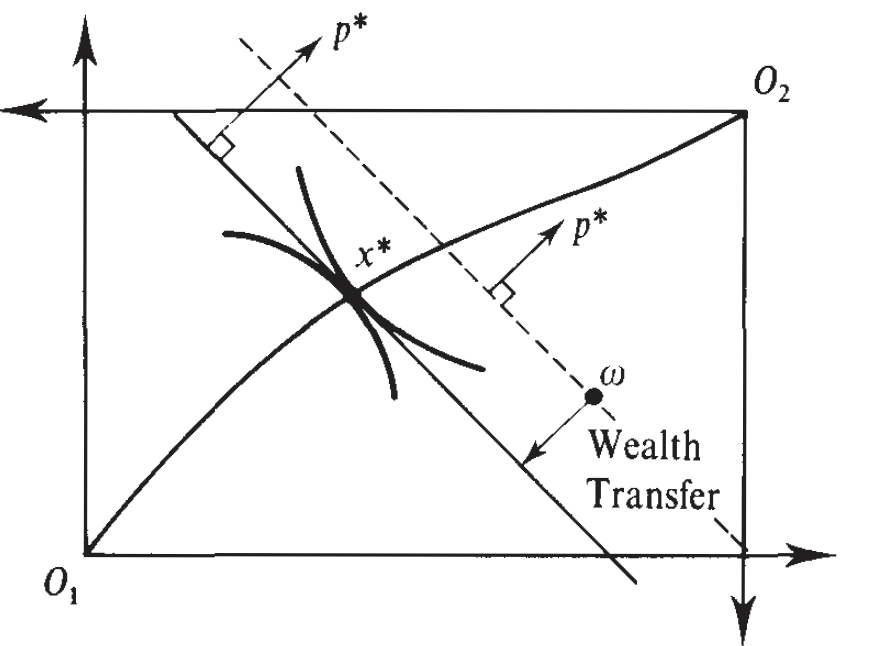
\includegraphics[width=0.4\linewidth]{figures/2ndFTWE.png}
			\caption{The Second Fundamental Theorem of Welfare Economics}
		\end{figure*}
		
		\begin{remark}
			In fact, if all commodities can be easily transferred, then we could equally well move the endowment vector directly to allocation $x^*$ instead of lump-sum transfer. From this new endowment point, the Walrasian equilibrium involves no trade.
		\end{remark}
		
		\newpage
		\subsection{The One Consumer, One Producer Economy}
			\paragraph{Economy Setup} Assume there are two \ul{price taking} agents: one consumer and one producer in the economy. There are two goods $x_1$ and $x_2$ in the economy.
			
			\begin{remark}
				It might be unreasonable to assume the single consumer and producer are price-takers. However, this can be explained as the interaction of a normative representative consumer and the whole industry (again, firm behaviours are always linearly additive).
			\end{remark}
			
			\paragraph{Consumer} The consumer has initial endowment of $\overline{L}$ units $x_1$ (leisure/working hours), and no endowment of $x_2$. Further, assume the consumer has \ul{continuous, convex, and strongly monotone} preference $\pref$ on the consumption set $X=\R^2_+$.
			\paragraph{Firm} The firm produces commodity $x_2$ with inputs $x_1$ via production function $f(\cdot)$, which is assumed to be \ul{increasing and strictly concave}. Moreover, the firm is owned by the consumer and all of its profit will be given to the consumer.
			\paragraph{Optimizations} Both firm and consumer are assumed to be price takers. Given the price vector $(p, w) \in \R^2_{++}$, the firm is assumed to be profit-maximizing:
			\begin{equation}
				\max_{z \in \R_+}\ pf(z) - w z
			\end{equation}
			Let $\pi(p, w)$ denote firm's profit, $z(p, w)$ and $q(p, w)$ denote the $\argmax$ and $f \circ \argmax$, respectively. The consumer is assumed to solve
			\begin{equation}
				\max_{(x_1, x_2) \in \R^2_+}\ u(x_1, x_2)\ s.t.\ p x_1 \leq w(\overline{L} - x_2) + \pi(p, w)
			\end{equation}
			The demand for the consumer is written as $(x_1(w, p), x_2(w, p))$.
			
			\paragraph{Walrasian Equilibrium} For a price vector $(w^*, p^*)$ to support a competitive equilibrium, the markets must be cleared at consumer's and firm's maximizers:
			\begin{align}
				z(w^*, p^*) &= \overline{L} - x_1(w^*, p^*) \\
				q(w^*, p^*) &= x_2(w^*, p^*)
			\end{align}
			
			\paragraph{Graphical Representation} Leisure and consumption levels are measured from the origin denoted $O_c$ at the lower-left hand corner of the diagram, which is determined by letting the length of the segment $[O_c, O_f]$ equal $\overline{L}$, the total labor endowment.
			
			\begin{figure*}[h]
				\centering
				\begin{subfigure}{.45\textwidth}
					\centering
					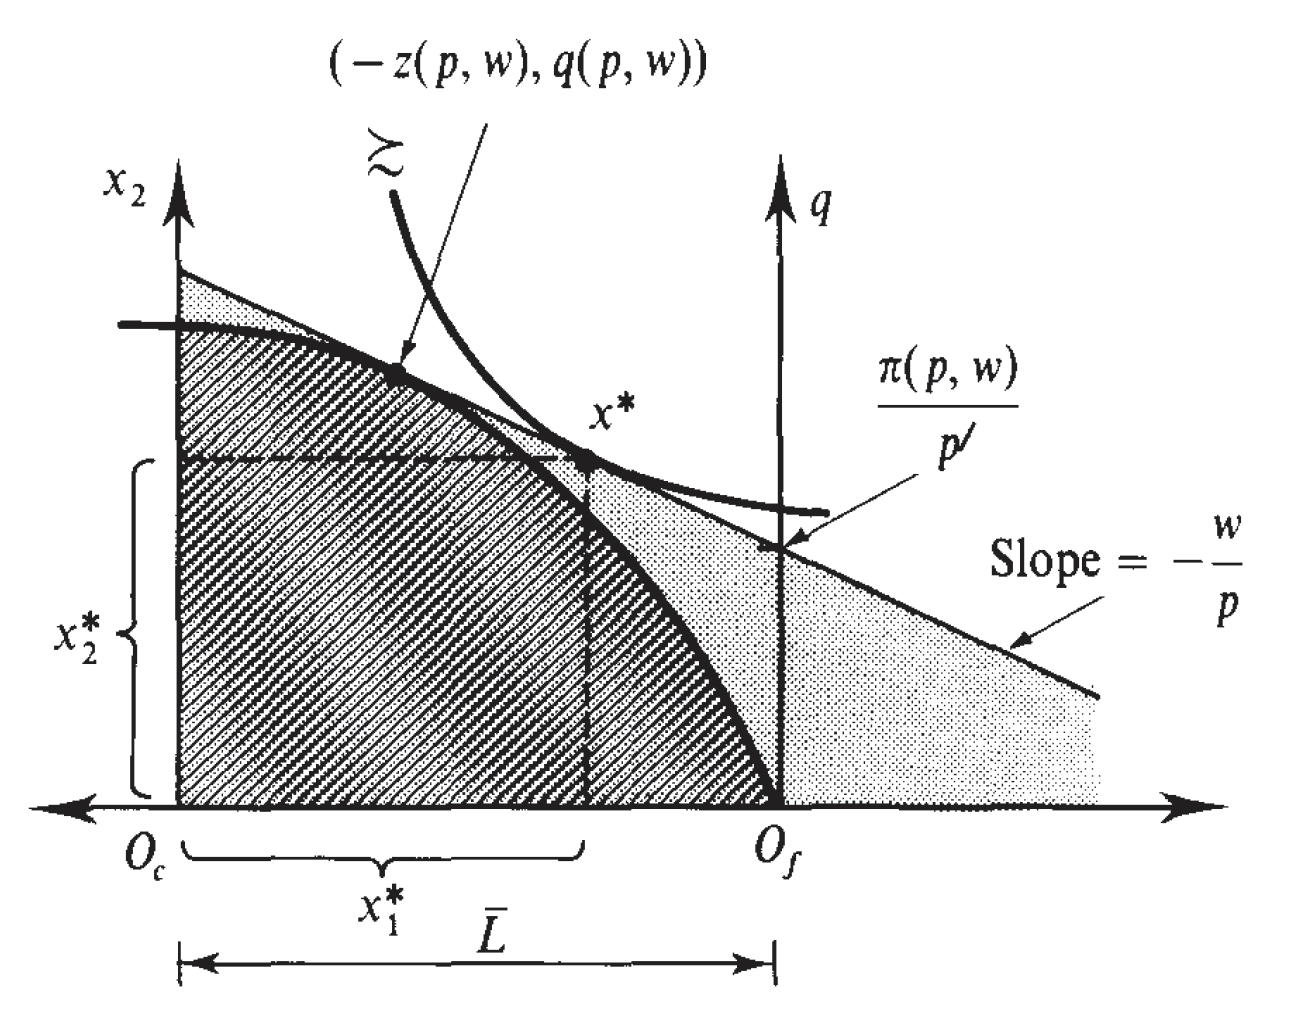
\includegraphics[width=\linewidth]{figures/1C1P_not_eq}
					\caption{A Non-Equilibrium Price Vector}
				\end{subfigure}
				\begin{subfigure}{.45\textwidth}
					\centering
					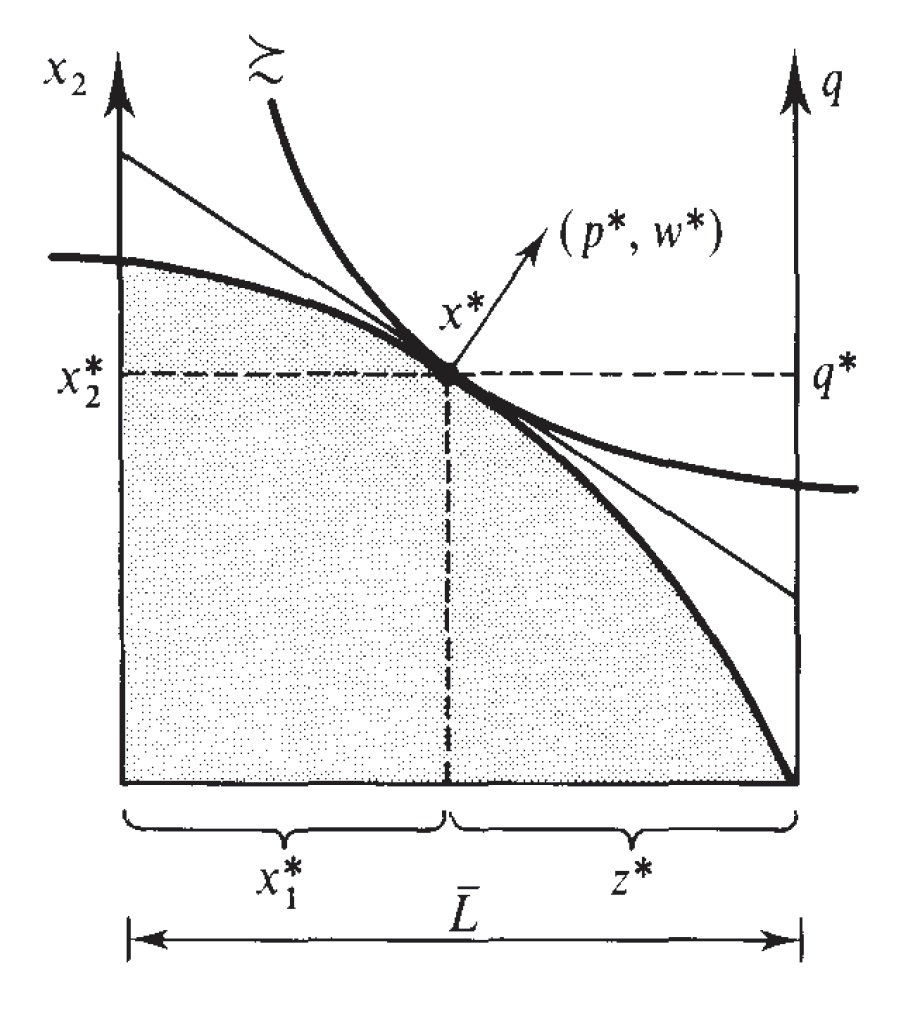
\includegraphics[width=0.75\linewidth]{figures/1C1P_eq}
					\caption{An Equilibrium Price Vector}
				\end{subfigure}
			\end{figure*}
			
			\begin{remark}
				A particular consumption-leisure combination can arise in a competitive equilibrium \ul{if only if} it maximizes the consumer's utility subject to the economy's technological and endowment constraints.
			\end{remark}
			
			\begin{corollary}[The First and Second Fundamental Theorem of Welfare Economics]
				Any Walrasian equilibrium is Pareto optimal, and the Pareto optimal allocation is supportable as a Walrasian equilibrium.
			\end{corollary}
			
			\begin{remark}
				For the second fundamental theorem to hold, the production set must be convex, but this is not required by the first fundamental theorem.
			\end{remark}
			
			\begin{figure*}[h]
				\centering
				\begin{subfigure}{.45\textwidth}
					\centering
					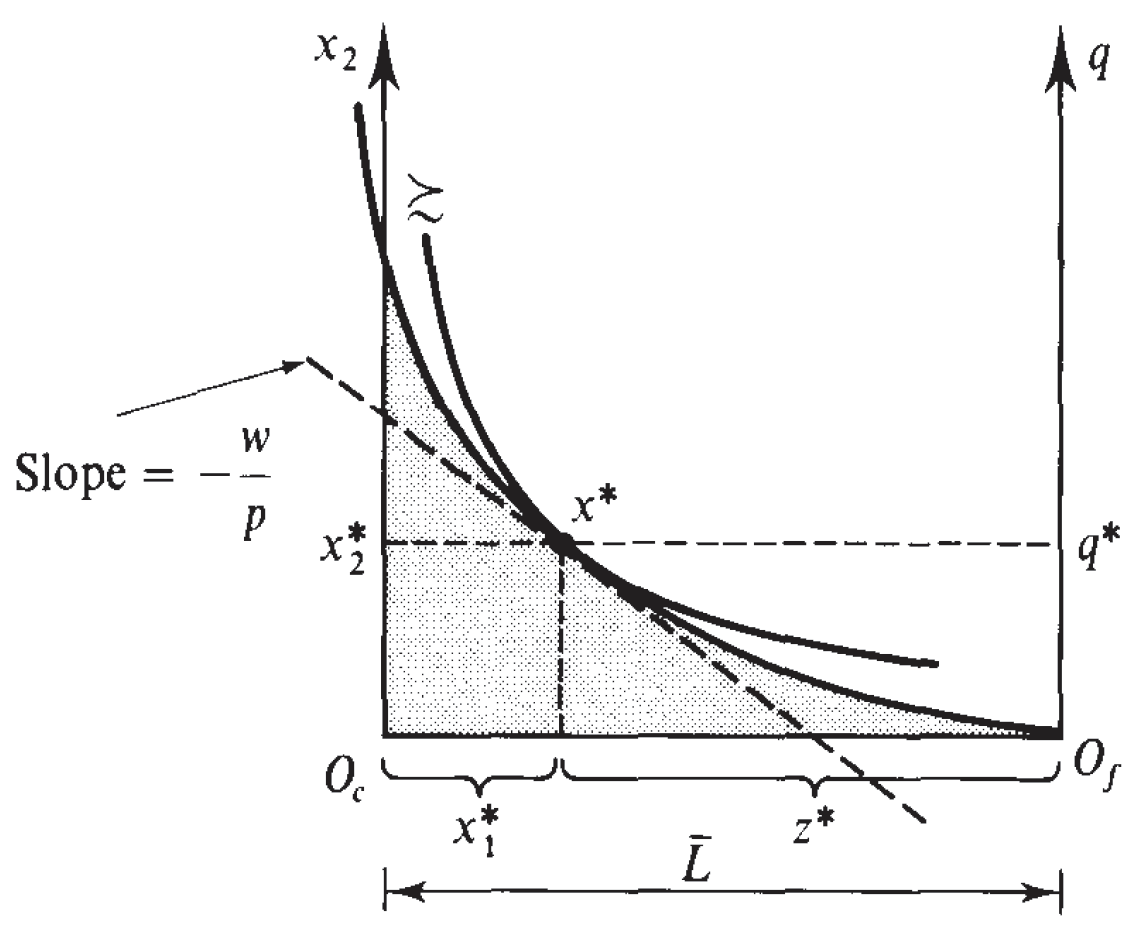
\includegraphics[width=\linewidth]{figures/fail_2FTWE}
					\caption{Failure of the Second Welfare Theorem with a Non-convex Technology}
				\end{subfigure}
				\begin{subfigure}{.45\textwidth}
					\centering
					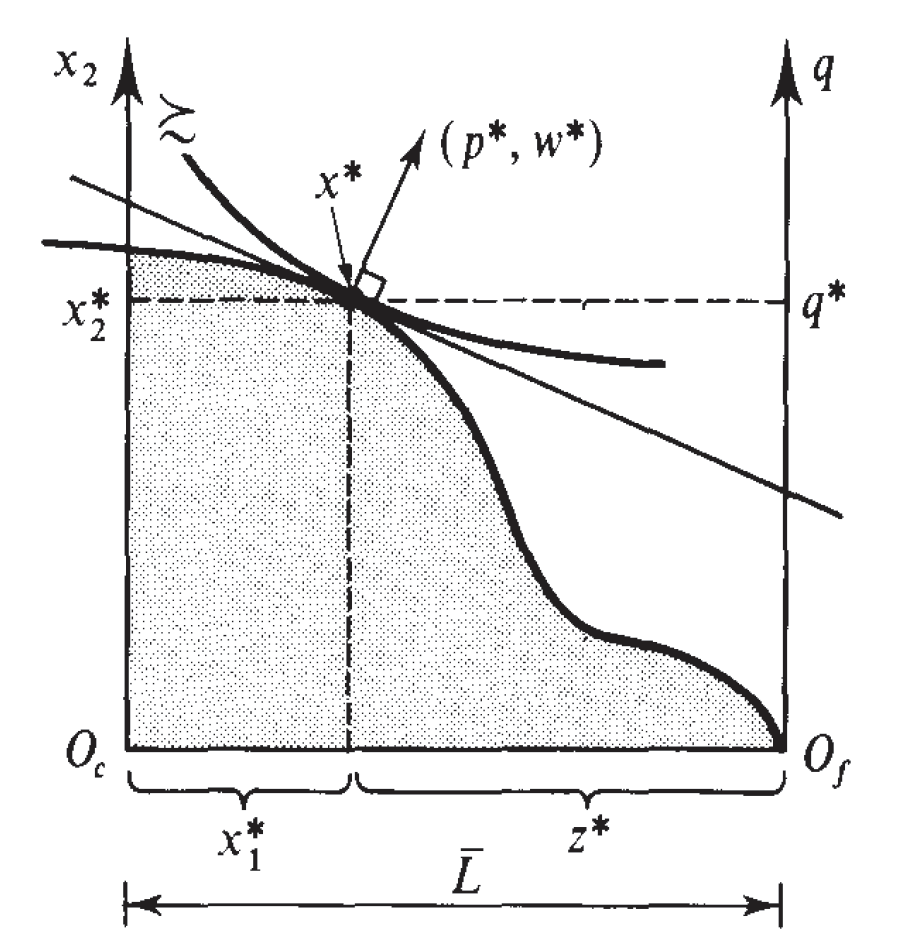
\includegraphics[width=0.8\linewidth]{figures/succ_1FTWE}
					\caption{The First Welfare Theorem Applies even with a Non-convex Technology.}
				\end{subfigure}
			\end{figure*}
	
		\subsection{The $2 \times 2$ Production Model}
			\subsubsection{Economy Setup(General)}
			\paragraph{Firms} There are $J$ price-taking firms each produces one type of product using $L$ primary inputs/factors, $z_j \in \R^L_+$ via production function $f_j: \R^L_+ \to \R_+$. $f_j$ is assumed to be \ul{concave, strictly increasing and differentiable}. The final product of firm $j$ is sold on the world market at price $p_j$.
			
			\begin{assumption}
				We assume the size of this economy is relatively small so the production decisions of firms within the economy does not affect the world price $p$.
			\end{assumption}			

			\paragraph{Consumers} Each consumer has initial endowment $(z_{\ell i})_\ell \in \R^L_{++}$. Consumers are selling their initial endowment to firms at factor price vector $w$. For each commodity $\ell$, let $\overline{z}_\ell := \sum_{I=1}^I z_{\ell i}$ denote the total endowment of commodity $\ell$ in the economy.
			
			\begin{assumption}
				We assume there are no intermediate goods, and consumers do not consume input factors directly.
			\end{assumption}
			
			\begin{remark}
				Output is sold in world markets. Factors, on the other hand, are immobile and must be used for production within the country.
			\end{remark}
			
			\begin{proposition}
				When $w \gg 0$, consumers supply all their endowments to the producers.
			\end{proposition}
			
			\begin{remark}
				An equilibrium can be characterized by $L(J+1)$ variables, a matrix $[z^*_{\ell j}] \in M_{L \times J}(\R)$ representing the allocation of initial endowments among firms and a price vector $w \in \R^L_{++}$. Note that at any such equilibrium, all firms are optimizing
				\begin{equation}
					\forall j \in [J],\ z^*_j \in z_j(w, p)
				\end{equation}
				and all markets clear
				\begin{equation}
					\forall \ell \in [L],\ \sum_{j\in [J]} z^*_{\ell j} = \overline{z}_{\ell}
				\end{equation}
			\end{remark}
			
			\begin{proposition}
				Given exogenous product price in the world market $p$. For an equilibrium with interior allocation, that is $z^*_j \gg 0\ \forall j \in [J]$, and strictly positive factor price vector $w \gg 0$, the allocation satisfies the necessary (also sufficient because of the concavity of $f_j$) of firms' profit maximization problem,
				\begin{equation}
					\forall (\ell, j) \in [L]\times [J],\ 
					p_{j} \frac{\partial f_{j}\left(z_{j}^{*}\right)}{\partial z_{\ell j}}=w_{\ell}^{*}
				\end{equation}
				and all $L$ markets are cleared,
				\begin{equation}
					\forall \ell \in [L],\ 
					\sum_{j} z_{\ell j}^{*}=\overline{z}_{\ell}
				\end{equation}
				and the equilibrium level of products is $q^*_j = f_j(z_j^*)$ for every $j$. And above $L(J+1)$ equations characterize the $L(J+1)$ equilibrium variables.
			\end{proposition}
			
			\subsubsection{Special Case: $L=J=2$, the $2 \times 2$ Production Model}
			\begin{assumption}
				Assume each firm has $f_j(\cdot)$ homogeneous of degree 1, that's, the technology is \ul{constant return to scale}.
			\end{assumption}
			
			\paragraph{Unit Production} For each $j \in \{1, 2\}$, given factor price vector $w = (w_1, w_2)$, let $c_j(w)$ denote the minimal cost of producing \ul{1 unit} of product $x_j$. Let $a_j(w) = (a_{1j}(w), a_{2j}(w))$ denote the $\argmin$, and assume they are unique. By the constant return to scale property, the cost minimizing factors for $q$ unit of output would be exactly $q a_j(w)$.
			
			\begin{proof}
				Consider 
				\begin{align}
					&\argmin_{z \geq 0} w \cdot z\ s.t.\ f(z) \leq q \\
					&= \argmin_{z \geq 0} w \cdot z\ s.t.\ \frac{f(z)}{q} \leq 1 \\
					&= \argmin_{z \geq 0} w \cdot z\ s.t.\ f\left(\frac{z}{q}\right) \leq 1 \\
					&= \argmin_{z \geq 0} q w \cdot \frac{z}{q}\ s.t.\ f\left(\frac{z}{q}\right) \leq 1 \\
					&= q \argmin_{z/q \geq 0} q w \cdot \frac{z}{q}\ s.t.\ f\left(\frac{z}{q}\right) \leq 1 \\
					&= q \argmin_{z/q \geq 0} w \cdot \frac{z}{q}\ s.t.\ f\left(\frac{z}{q}\right) \leq 1 \\
					&= q \argmin_{z \geq 0} w \cdot z\ s.t.\ f(z) \leq 1 = q a(w)
				\end{align}
			\end{proof}
			
			\begin{proposition}
				By Shephard's lemma/ the envelope theorem,
				\begin{equation}
					a_j(w) = \nabla_w c_j(w)
				\end{equation}
			\end{proposition}
			
			\begin{definition}
				The \textbf{Pareto set of factor allocations} is the set of factor allocations $(a_j)$ at which it is not possible, with the given total factor endowments, to produce more of one good without producing less of the other.
			\end{definition}
			
			\begin{figure*}[h]
				\centering
				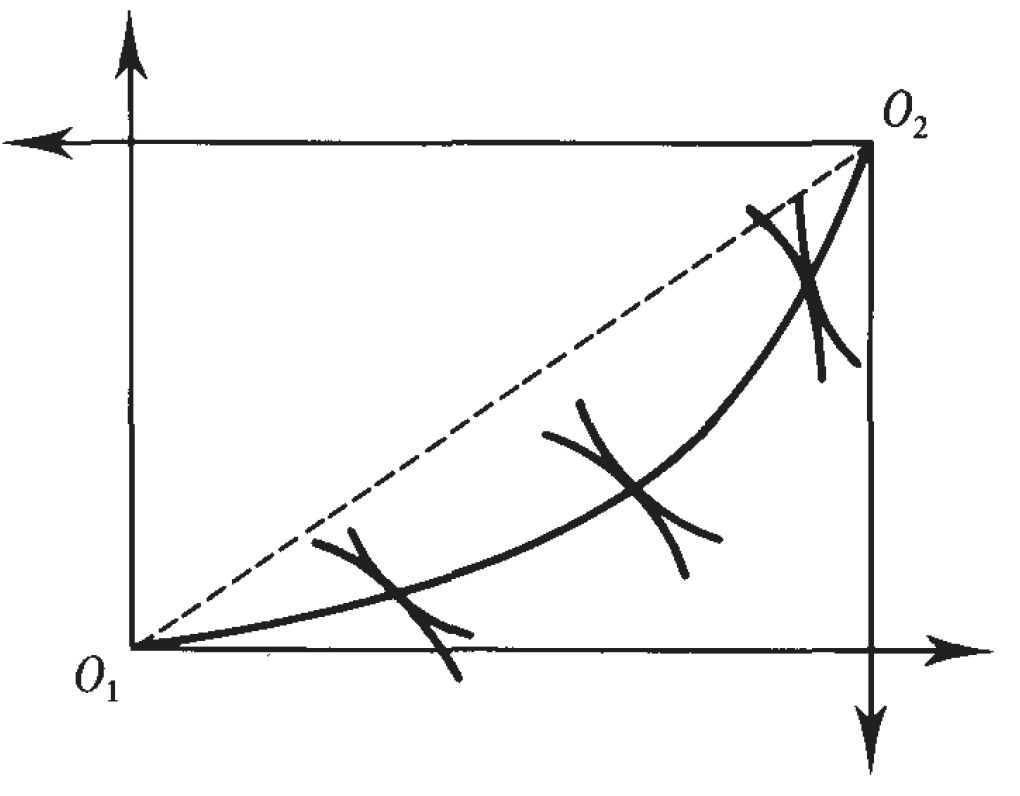
\includegraphics[width=0.3\linewidth]{figures/pareto_prod_set}
				\caption{The Pareto Set of Factor Allocations}
			\end{figure*}
			
			\begin{definition}
				The production of good 1 is \textbf{relatively more intensive} in factor 1 than the production of good 2 if
				\begin{equation}
					\frac{a_{11}(w)}{a_{21}(w)} > \frac{a_{12}(w)}{a_{22}(w)}
				\end{equation}
				\ul{for all factor prices $w$}.
			\end{definition}
			
			\paragraph{Equilibrium Factor Prices} Suppose we have an interior equilibrium (i.e. the equilibrium is \emph{not} specialized), and given the constant return assumption (so unit cost $c_j$ is precisely the marginal cost), then the necessary condition for firm $j$ to optimize is
			\begin{equation}
				c_j(w_1, w_2) = p_j
			\end{equation}
			Thus the set of factor prices satisfying the competitive equilibrium is 
			\begin{equation}
				w^* \in \bigcap_j \left \{
				(w_\ell) \in \R^L_{++}: c_j(w_\ell) = p_j
				\right \}
			\end{equation}
			\begin{remark}
				In the $2 \times 2$ case, assuming product 1 is more intensive in factor 1, when curve $c_1(w)=p_1$ and $c_2(w)=p_2$ intersect, $c_1(w)=p_1$ is steeper because of Shephard's lemma. As a result, the intersection of those curves is unique.
			\end{remark}
			
			\begin{figure*}[h]
				\centering
				\begin{subfigure}{.45\textwidth}
					\centering
					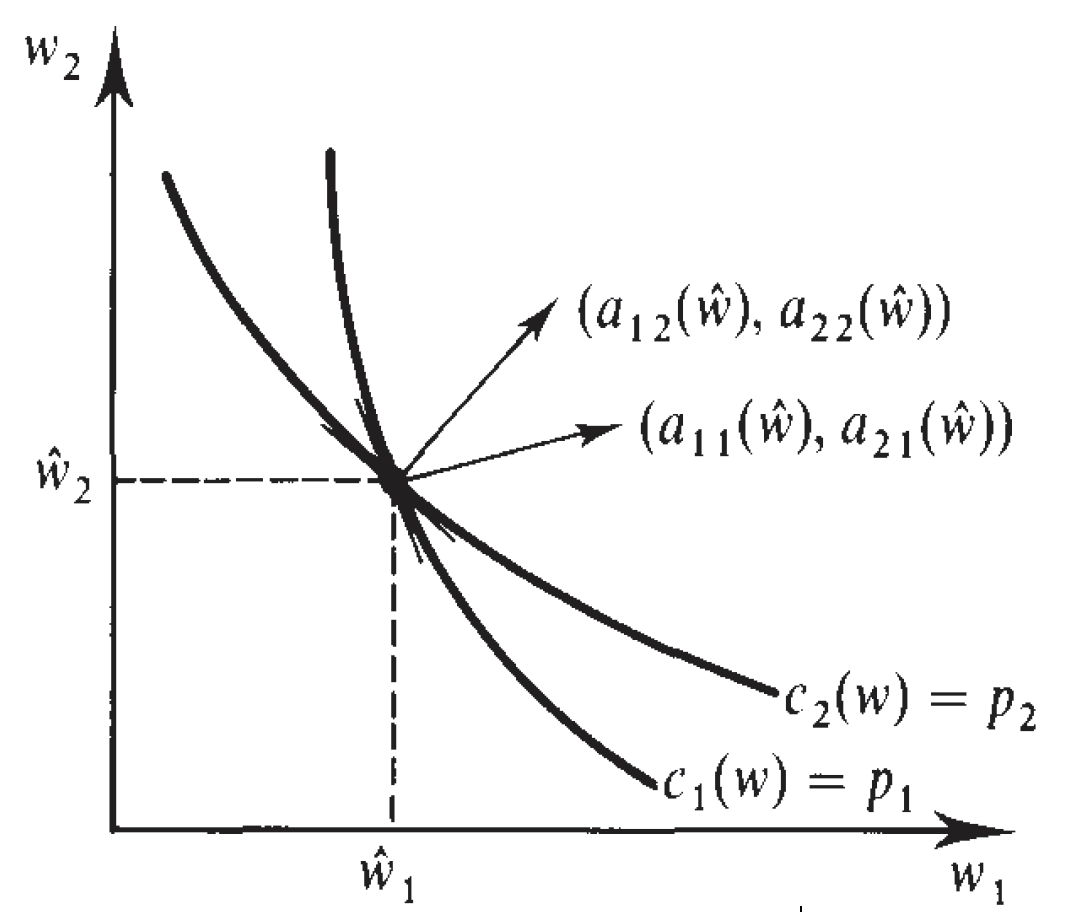
\includegraphics[width=0.7\linewidth]{figures/equilibrium_factor_prices}
					\caption{The Equilibrium Factor Prices}
				\end{subfigure}
				\begin{subfigure}{.45\textwidth}
					\centering
					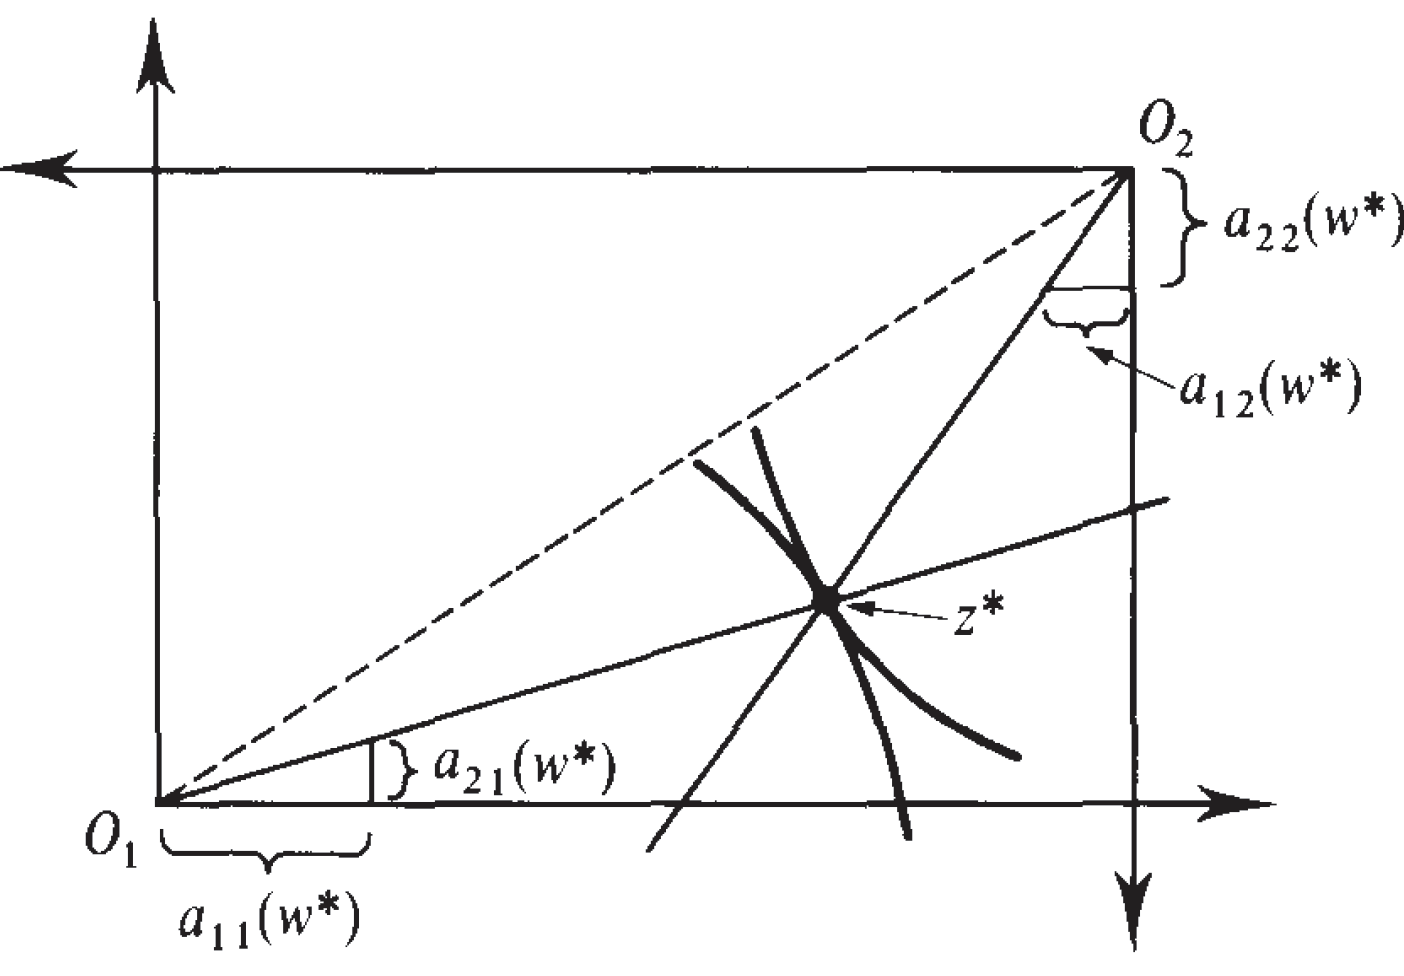
\includegraphics[width=1\linewidth]{figures/equilibrium_factor_allocation}
					\caption{The Equilibrium Factor Allocation}
				\end{subfigure}
			\end{figure*}
			
			\paragraph{Equilibrium Factor Allocation} Given the constant return to scale nature of technologies, the ratio of input factors at equilibrium equals $\frac{a_{1j}}{a_{2j}}$ for each firm $j$. Given equilibrium factor price vector $w$, the equilibrium factor allocation $(z^*_{\ell j})$ is given by solving
			\begin{equation}
				\frac{z_{11}^{*}}{z_{21}^{*}}=\frac{a_{11}\left(w^{*}\right)}{a_{21}\left(w^{*}\right)} \quad \text { and } \quad \frac{z_{12}^{*}}{z_{22}^{*}}=\frac{a_{12}\left(w^{*}\right)}{a_{22}\left(w^{*}\right)}
			\end{equation}
			
			\begin{remark}
				The equilibrium factor prices depend only on the technologies of the two firms and on the output prices $p$, and independent from the initial endowment of factors.
			\end{remark}
			
			\subsubsection{Comparative Statics: Change in Output Price}
			\begin{theorem}[Stolper-Samuelson Theorem]
				In the $2 \times 2$ production model with factor intensity assumption, if $p_j$ increases, the equilibrium price of the factor more intensively used in the production of good $j$ increases, while the price of the other factor decreases, assuming interior equilibrium both before and after the price change.
			\end{theorem}
			
			\begin{proof}
				Differentiate both sides of optimal conditions for all firms $c_j(w_1, w_2) = p_j$ gives
				\begin{equation}
					d p_j = \nabla_w c_j(w^*) dw
				\end{equation}
				By the Shephard's lemma
				\begin{equation}
					dp_j = \begin{pmatrix}a_{1j}(w^*)\\ a_{2j}(w^*)\end{pmatrix} \cdot dw
				\end{equation}
				in matrix notation
				\begin{equation}
					d p=\underbrace{
					\left[ \begin{array}{ll}{a_{11}\left(w^{*}\right)} & {a_{21}\left(w^{*}\right)} \\ {a_{12}\left(w^{*}\right)} & {a_{22}\left(w^{*}\right)}\end{array}\right]
					}_{A}
					 d w
				\end{equation}
				note that $|A| > 0$ because of the factor intensity assumption. Therefore, $A$ is invertible and 
				\begin{align}
					dw &= A^{-1} dp \\
					\iff dw &= \frac{1}{|A|} \left[ \begin{array}{cc}{a_{22}\left(w^{*}\right)} & {-a_{21}\left(w^{*}\right)} \\ {-a_{12}\left(w^{*}\right)} & {a_{11}\left(w^{*}\right)}\end{array}\right] dp
				\end{align}
				Take $dp = (\varepsilon, 0)$ for some $\varepsilon > 0$, 
				\begin{equation}
					dw = \frac{\varepsilon}{|A|} 
					\begin{pmatrix}
						a_{22}(w^*)\\
						-a_{12}(w^*)
					\end{pmatrix}
				\end{equation}
			\end{proof}
			
			\begin{figure*}[h]
				\centering
				\begin{subfigure}{0.45\textwidth}
					\centering
					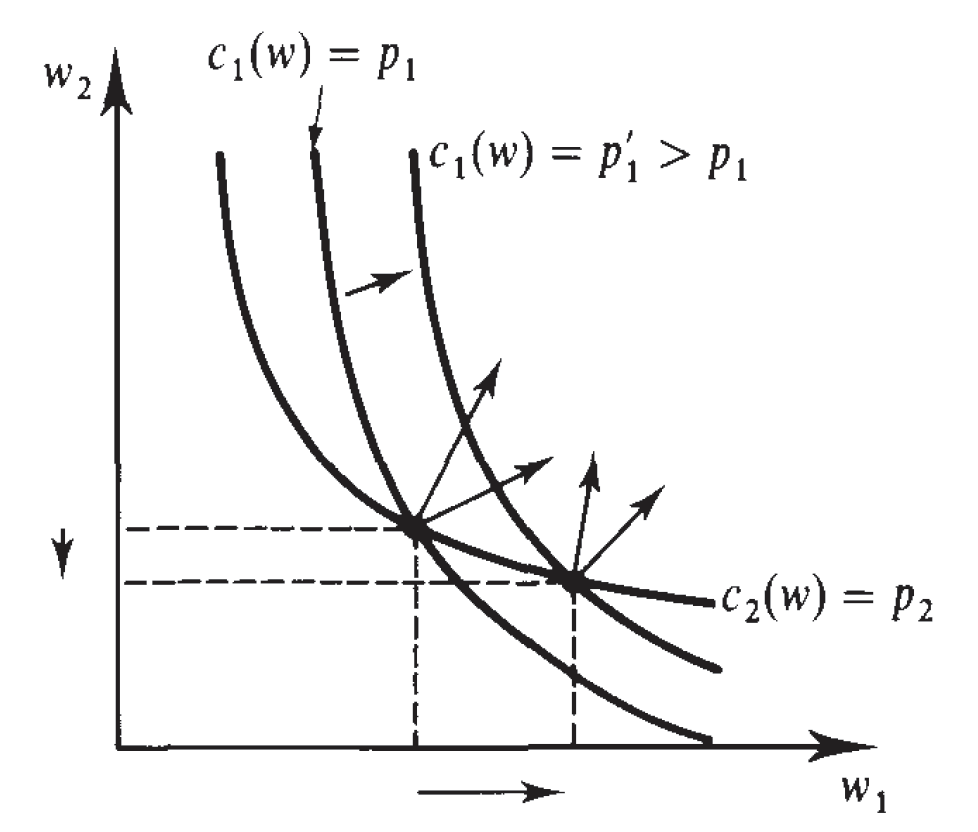
\includegraphics[width=.7\linewidth]{figures/Stolper_Samuelson}
					\caption{Changes in Factor Prices}
				\end{subfigure}
				\begin{subfigure}{0.45\textwidth}
					\centering
					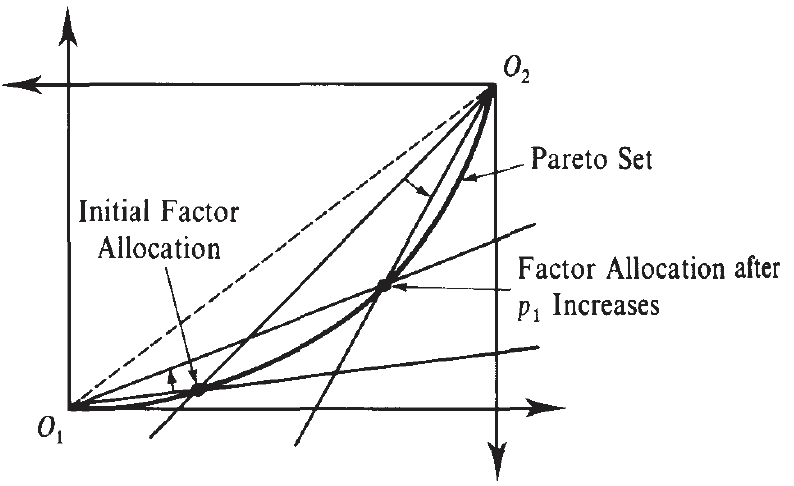
\includegraphics[width=\linewidth]{figures/Stolper_Samuelson_2}
					\caption{Changes in Factor Allocation}
				\end{subfigure}
			\caption{The Stolper-Samuelson Theorem}
			\end{figure*}
			
			\subsubsection{Comparative Statics: Change in Endowments}
			\begin{remark}
				As noted before, the equilibrium factor prices are left unaffected when the endowment changes.
			\end{remark}
			
			\begin{theorem}[Rybcszynski Theorem]
				In the $2 \times 2$ production model with the factor intensity assumption, if the endowment of a factor increases, then the production of the good that uses this factor relatively more intensively increases and the production of the other good decreases (assuming interior equilibria both before and after the change of endowment).
			\end{theorem}
			
			\begin{figure*}[h]
				\centering
				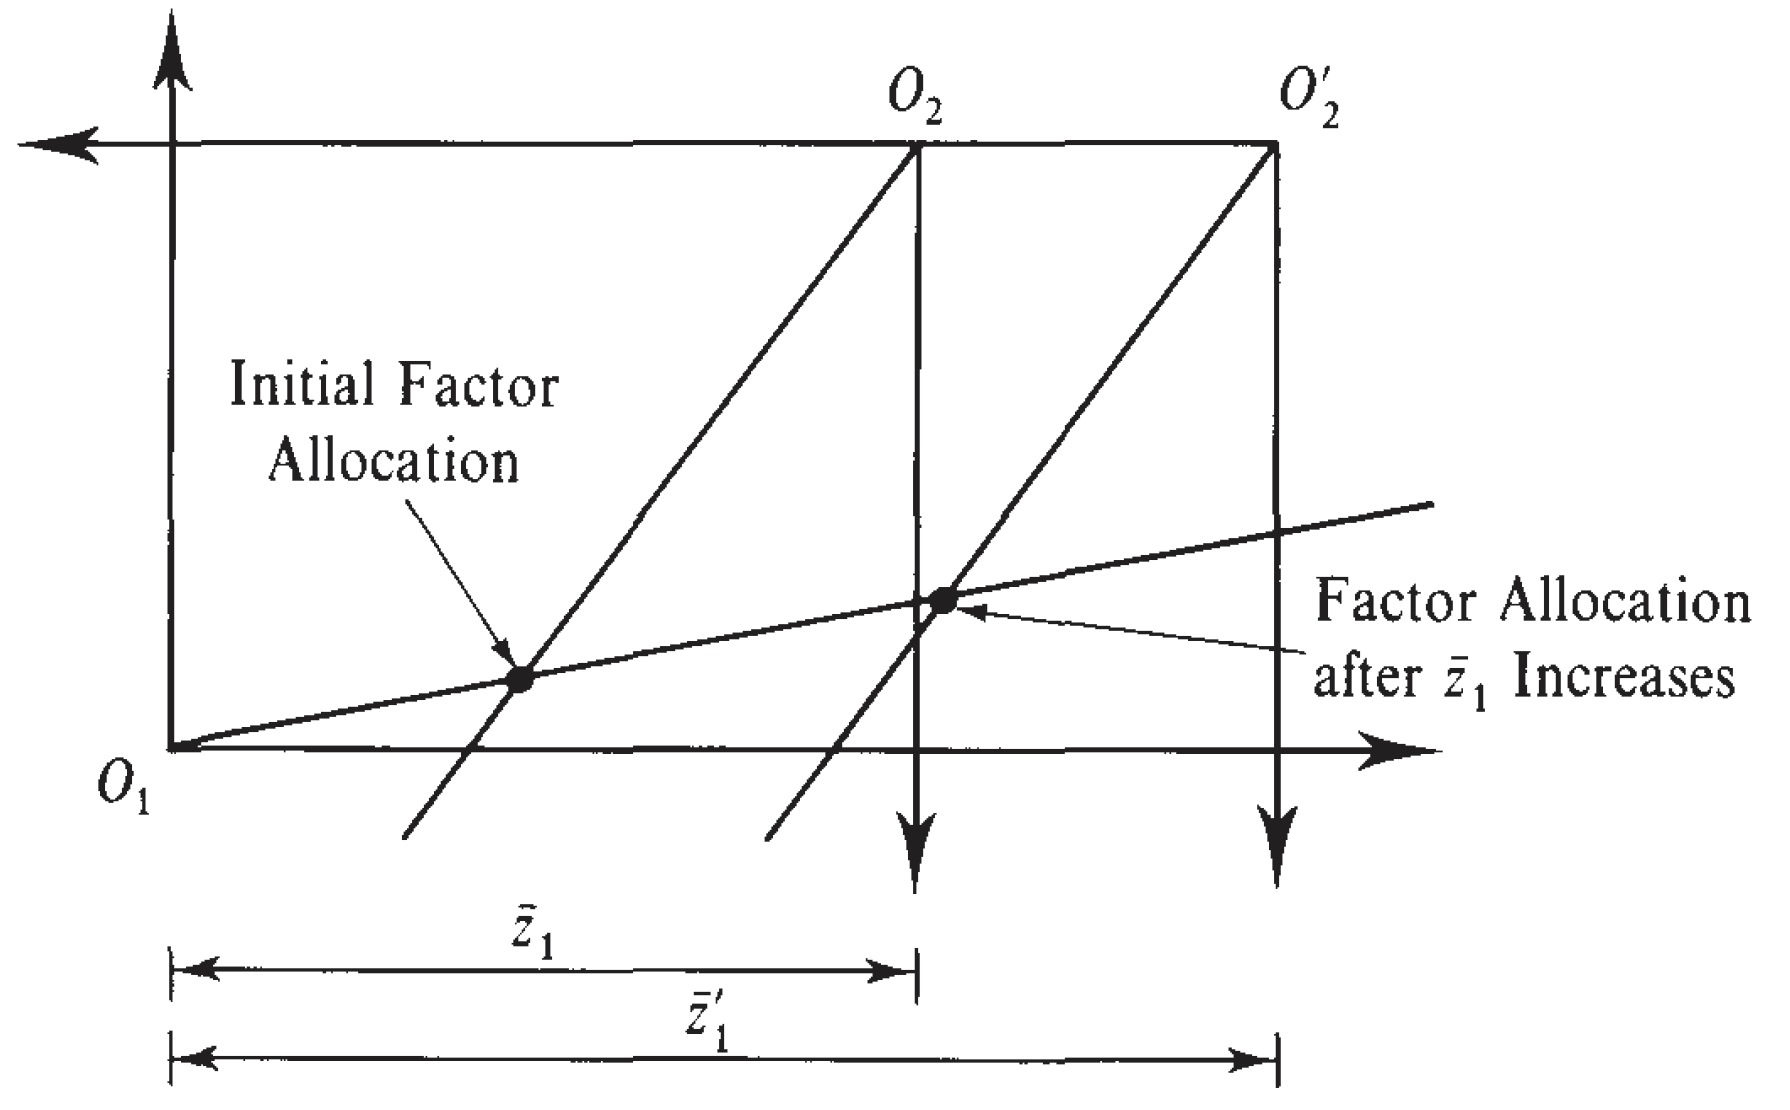
\includegraphics[width=0.6\linewidth]{figures/Rybcszynski}
				\caption{The Rybcszynski Theorem}
			\end{figure*}
			
			\begin{remark}
				Consider a more general case with $L$ input factors and $J$ firms, note that we need to solve the $L$ factor prices from $J$ optimal conditions of firms. If $L > J$, then there are too many unknowns and we cannot hope that the zero-profit conditions alone will determine the factor prices. The total factor endowments will play a role. If $J > L$, then there are too many equations and, for typical world prices, they cannot all be satisfied simultaneously. What this means is that the economy will specialize in the production of a number of goods equal to the number of factors $L$. Therefore, in general, we examine cases when $J=L$.
			\end{remark}
	\section{Chapter 16. Equilibrium and Its Basic Welfare Properties}
		\subsection{Definitions}
		\begin{remark}
			The \textbf{disposal technology} can be written as $Y_1 = -\R^2_+$.
		\end{remark}
		
		\begin{definition}
			An economy is a \textbf{pure exchange economy} if its only technological possibility is the free disposal technology, $Y_j = -\R^L_+\ \forall j$. 
		\end{definition}
		
		\begin{definition}[16.B.1.a]
			An \textbf{allocation} $(x, y) \equiv \langle (x_i), (y_j) \rangle$ is a specification of a consumption vector $x_i \in X_i$ for each consumer $i$ and a production vector $y_j \in Y_j$ for each firm $j$.
		\end{definition}
		
		\begin{definition}[16.B.1.b]
			An allocation $(x, y)$ is \textbf{feasible} if 
			\begin{equation}
				\sum_i x_i = \overline{\omega} + \sum_j y_j
			\end{equation}
			we denote the set of feasible allocations by 
			\begin{equation}
				A = \left\{(x, y) \in \prod_i X_i \times \prod_j Y_j: \sum_i x_i = \overline{\omega} + \sum_j y_j \right\} \subset \R^{L(I+J)}
			\end{equation}
		\end{definition}
		
		\begin{definition}[16.B.2]
			A feasible allocation $(x, y)$ is \textbf{Pareto optimal/efficient} if there is no other feasible allocation $(x', y')$ such that $x_i' \pref_i x_i$ for all $i$ and $x_i' \succ_i x_i$ for some $i$.
		\end{definition}
		
		\subsection{Private Ownership Economies}
		\paragraph{Economy} In a private ownership economy, every good $\ell$ is traded on a market consisting of price-taking firms and consumers. The wealth of consumers are from their initial endowments (in terms of commodities) and dividend from firms' profits based on their ownerships of firms.
		
		\paragraph{Endowments} Consumer $i$ possesses an initial endowment vector $\omega_i \in \R^L$ and a claim $\theta_{ij} \in [0, 1]$ to firm $j$'s profit. Hence, $\forall j,\ \sum_i \theta_{ij} = 1$.
		
		\begin{remark}
			A private ownership economy can be constructed as
			\begin{equation}
				\mc{E} = \left \langle
					\left \{ (X_i, \pref_i) \right \}_{i=1}^I,
					\{Y_j\}_{j=1}^J,
					\{(\omega_i, \{\theta_{ij}\}_j)\}_{i=1}^I
				\right \rangle
			\end{equation}
		\end{remark}
		
		\begin{definition}[16.B.3]
			Given a private ownership economy $\mc{E}$ and an allocation $(x^*, y^*)$ and a price vector $p$ constitute a \textbf{Walrasian (or competitive) equilibrium} if
			\begin{enumerate}[(i)]
				\item For $j$, $y_j^*$ maximizes profit in $Y_j$; that is,
				\begin{equation}
					p \cdot y_j \leq p \cdot y_j^*\ \forall y_j \in Y_j
				\end{equation}
				\item For every $i$, $x_i^*$ is maximal for $\pref_i$ in the budget set
				\begin{equation}
					\left\{
					x_i \in X_i: p \cdot x_i \leq p \cdot \omega_i + \sum_i \theta_{ij} p \cdot y_j^*
					\right\}
				\end{equation}
				\item Market clears $\sum_i x_i^* = \overline{\omega} + \sum_j y_j^*$.
			\end{enumerate}
		\end{definition}
		
		\begin{remark}
			The second defining property of Walrasian equilibrium is equivalent to 
			\begin{equation}
				\forall i \in [I],\ \forall x_i \in X_i,\ x_i \succ_i x_i^* \implies p \cdot x_i > p \cdot \omega_i + \sum_i \theta_{ij} p \cdot y_j^*
			\end{equation}
		\end{remark}
		
		\begin{definition}
			A generalization of price vector $p$ is called a \textbf{price system}. A typical price system is a \ul{linear continuous} mapping $\varphi: X \to \R$.
		\end{definition}
		
		\paragraph{Price Equilibria with Transfers} We can imagine a situation where a social planner is able to carry out (lump-sum) redistributions of wealth, and where society's aggregate wealth can therefore be redistributed among consumers in any desired manner.
		
		\begin{definition}[16.B.4]
			Given an economy specified by $\langle \{(X_i, \pref_i)\}_i, \{Y_j\}_j, \omega \rangle$, an allocation $(x^*, y^*)$ and a price vector $p$ constitute a \textbf{price equilibirium with transfers} if there is an assignment of wealth levels $(w_i)$ with $\sum_i w_i = p \cdot \overline{\omega} + \sum_j p \cdot y_j^*$ such that
			\begin{enumerate}[(i)]
				\item $p \cdot y_j \leq p \cdot y_j^*\ \forall y_j \in Y_j$;
				\item $\forall x_i \in X_i,\ x_i \succ_i x_i^* \implies p \cdot x_i > w_i$;
				\item $\sum_i x_i^* = \overline{\omega} + \sum_j y_j^*$.
			\end{enumerate}
		\end{definition}
		
		\begin{remark}
			Note that a Walrasian equilibrium is a special case of an equilibrium with transfers. It amounts to the case which, for every $i$, consumer $i$'S wealth level is determined by the initial endowment vector $\omega_i$ and by the profit shares $[\theta_{ij}]$ without any further wealth transfers, that is, where $w_i = p \cdot \omega_i + \sum_{j} \theta_{ij} p \cdot y_j^*$ for every $i \in [I]$.
		\end{remark}
		
		\subsection{The First Fundamental Theorem of Welfare Economics}
		
		\begin{remark}
			For the first welfare theorem to hold, we only assume the local nonsatiation of preferences without appealing to any convexity assumption.
		\end{remark}
		
		\begin{definition}
			The preference relation $\pref_i$ on the consumption set $(X_i, d)$ is \textbf{locally nonsatiated} if for every $x_i \in X_i$ and every $\varepsilon$, there is an $x_i' \in X_i$ such that $d(x_i', x_i) \leq \varepsilon$ and $x_i' \succ_i x_i$.
		\end{definition}
		
		\begin{theorem}[The First Fundamental Theorem of Welfare Economics]
			In any private ownership economy where the set of consumers is finite, and all consumers preferences are \ul{locally nonsatiated}, then all Walrasian equilibrium allocation is Pareto efficient.
		\end{theorem}
		
		\begin{proof}[Proof (by Contradiction)]
			Suppose $\{\langle x^*, y^* \rangle, \varphi^*\}$ is a Walrasian equilibrium. Hence, $x^*_i$ solves the consumers' maximization problem,
			\begin{equation}
				x_i \succ_i x_i^* \implies \varphi^*(x_i) > \varphi^*(x_i^*)\ \forall x_i \in X_i
			\end{equation}
			\begin{lemma}
				\begin{equation}
					x_i \pref_i x_i^* \implies \varphi^*(x_i) \geq \varphi^*(x_i^*)\ \forall x_i \in X_i
				\end{equation}
			\end{lemma}
			\begin{proof}[Proof (by Contradiction)]
				Suppose there exists $x_i \in X_i$ such that $x_i \pref_i x_i^*$ and $\varphi^*(x_i) < \varphi^*(x_i^*)$. By local nonsatiation of $\pref_i$, for each $n \in \N$, there exists a $x_i^n \in \mc{B}(\frac{1}{n}, x_i)$ such that $x_i^n \succ_i x_i$ and $(x_i^n) \to x_i$. Because of the continuity of $\varphi^*$, $(\varphi^*(x_i^n)) \to \varphi^*(x_i)$. Further, since $x_i^n \succ_i x_i \pref_i x_i^*$, $\varphi^*(x_i^n) > \varphi^*(x_i^*)\ \forall n \in \N$. However, the convergence of $(\varphi^*(x_i^n))$ implies there exists $N^* \in \N$ such that $\forall n > N^*,\ \varphi^*(x_i^n) < \varphi^*(x_i^*)$, which leads to a contradiction.
			\end{proof}
			Suppose $\langle x^*, y^* \rangle$ is not a Pareto optimal, then there exists another feasible allocation $\langle x', y' \rangle$ Pareto dominating $\langle x^*, y^* \rangle$. That is
			\begin{align}
				&\exists\ \varnothing \neq \mc{N} \subseteq [I],\ s.t.\ \forall I \in \mc{N},\ x_i' \succ_i x_i^* \\
				&\forall I \in \mc{E} := \mc{N}^c,\ x_i' \succsim_i x_i^*
			\end{align}
			By the maximization property, 
			\begin{equation}
				\sum_{I \in \mc{N}} \varphi^*(x_i') > \sum_{I \in \mc{N}} \varphi^*(x_i^*)
			\end{equation}
			and, by above lemma,
			\begin{equation}
				\sum_{I \in \mc{E}} \varphi^*(x_i') \geq \sum_{I \in \mc{E}} \varphi^*(x_i^*)
			\end{equation}
			which implies 
			\begin{align}
				\varphi^*\left(\sum_{I=1}^I x_i^* \right) &= 
				\sum_{I=1}^I \varphi^*(x_i') > \sum_{I=1}^I \varphi^*(x_i^*) \\
				&= \varphi^*(\overline{\omega}) + \sum_{j=1}^J \varphi^*(y_j^*)
				= \varphi^*(\overline{\omega}) + \varphi^*(\sum_{j=1}^J y_i^*) \\
				&= \varphi^*\left(\overline{\omega} + \sum_{j=1}^J y_i^* \right) \\
				&\implies \sum_{I=1}^I x_i^* > \overline{\omega} + \sum_{j=1}^J y_i^*
			\end{align}
			this leads to a contraction on the aggregate feasibility of allocation $\langle x', y' \rangle$.
		\end{proof}
		
		\begin{remark}
			Although the result of the first fundamental theorem seems from a weak premise, but, it implicitly incorporates two strong assumptions
			\begin{enumerate}[(i)]
				\item \emph{Universal price quoting of commodities} (market completeness);
				\item \emph{Price taking} by economic agents.
			\end{enumerate}
		\end{remark}
		
		\subsection{The Second Fundamental Theorem of Welfare Economics}
		\begin{definition}[16.D.1]
			Given an economy specified by $(\{(X_i, \pref_i)\}_{I=1}^I, \{Y_j\}_{j=1}^J, \overline{\omega})$, an allocation $(x^*, y^*)$ and a price vector $p \neq 0$ constitute a \textbf{price quasi-equilibrium with transfers} if there exists an assignment of wealth $(w_i)$ with $\sum_i w_i = p \cdot \overline{\omega} + \sum_j p \cdot y_j^*$ such that
			\begin{enumerate}[(i)]
				\item For every $j, y_j^*$ maximizes profits in $Y_j$; that is 
				\begin{equation}
					p \cdot y_j \leq p \cdot y_j^*\ \forall y_j \in Y_j
				\end{equation}
				\item \red{For every $i$, $x_i \succ_i x_i^* \implies p \cdot x_i \geq w_i$};
				\item $\sum_i x_i^* = \overline{\omega} + \sum_j y_j^*$.
			\end{enumerate}
		\end{definition}
		
		\begin{proposition}
			The second defining property of the quasi-equilibrium is a weaker that the counter-part of it in the definition of Walrasian equilibrium ($x_i \succ_i x_i^* \implies p \cdot x_i > w_i$). It is equivalent to the expenditure minimization on the set $\{x_i \in X: x_i \pref_i x_i^*\}$, that is
			\begin{equation}
				\forall x_i \in X_i,\ x_i \pref_i x_i^* \implies p \cdot x_i \geq p \cdot x_i^*
			\end{equation}
			\begin{proof}
				Given the local satiation assumption, $p \cdot x_i^* \geq w_i$ for every consumer. Further, the market clearance condition and the feasibility of wealth redistribution, $\sum_i p \cdot x_i^* = \sum_i w_i$. These two implies $p \cdot x_i^* = w_i$, which suggests 
				\begin{equation}
					x_i \succ_i x_i^* \implies p \cdot x_i \geq p \cdot x_i^*
				\end{equation}
				Show $x_i \sim_i x_i^* \implies p \cdot x_i \geq p \cdot x_i^*$. (By contradiction) Suppose there exists $x_i \sim_i x_i^*$ such that $p \cdot x_i < p \cdot x_i^*$. By local nonsatiation, there exists $x_i' \succ_i x_i \sim_i x_i^*$ such that $p \cdot x_i' < p \cdot x_i^*$, which leads to a contradiction.
			\end{proof}
		\end{proposition}
		
		\begin{theorem}[Separating Hyperplane Theorem]
			Let $A, B$ be two \ul{non-empty, disjoint and convex} subset of $\R^n$, then there exists a nonzero vector $v \in \R^n$ and $c \in \R$ such that 
			\begin{align}
				\forall x \in A,\ \langle x, v \rangle \geq c \\
				\forall x \in B,\ \langle x, v \rangle \leq c
			\end{align}
			That is, $(v, c)$ forms a hyperplane $\{x \in \R^n: \langle v, x \rangle = c\} \subset \R^n$ separating $A$ and $B$.
		\end{theorem}
		
		\begin{proposition}[16.D.1 The Second Fundamental Theorem of Welfare Economics: Part 1]
			Consider an economy $\mc{E}$, and suppose that \ul{every $Y_j$ is convex and every preference relation $\pref_i$ is convex and locally nonsatiated}. Then for every Pareto optimal allocation $(x^*, y^*)$, there is a price vector $p \neq 0$ (thus a linear and continuous price system $\varphi(x) := p \cdot x$) such that $(x^*, y^*, p)$ is a \emph{price quasi-equilibrium with transfers}.
		\end{proposition}
		
		\begin{proof}
			Suppose $(x^*, y^*)$ is a Pareto optimal allocation for economy $\mc{E}$.\\
			For each consumer $i$, define
			\begin{equation}
				V_i := \{x_i \in X_i: x_i \pref_i x_i^*\} \subset \R^L
			\end{equation}
			and the set of preferred aggregate consumption bundle
			\begin{equation}
				V := \sum_i V_i = \left \{
					\sum_i x_i \in \R^L:
					x_i \in V_i\ \forall i \in [I]
				\right \}
			\end{equation}
			and the aggregate production set
			\begin{equation}
				Y := \sum_j Y_j = \left \{
					\sum_j y_j \in \R^L:
					y_j \in Y_j\ \forall j \in [J]
				\right \}
			\end{equation}
			Hence, the set of attainable allocation is $Y + \{ \overline{\omega} \}$.
			\paragraph{Lemma 1} \emph{Every $V_i$ is convex.}
			\begin{proof}
				Let $x_i, x_i' \in V_i$, and $\alpha \in [0, 1]$. Since $\pref_i$ is complete, we assume $x_i \pref_i x_i'$ without loss of generality. Therefore $x_i$, as well as $x_i'$ itself, are in the upper contour set of $x_i'$. By the convexity of $\pref_i$, $\alpha x_i + (1 - \alpha) x_i' \pref_i x_i'$. By transitivity of $\pref_i$, $\alpha x_i + (1 - \alpha) x_i' \succ_i x_i^*$, which implies $\alpha x_i + (1 - \alpha) x_i' \in V_i$. Therefore, $V_i$ is convex.
			\end{proof}
			\paragraph{Lemma 2} \emph{$V$ and $Y + \{\overline{\omega}\}$ are convex.}
			\begin{proof}
				The lemma follows immediately from the fact that summations of convex sets are convex, and a singleton is trivially convex.
			\end{proof}
			\paragraph{Lemma 3} \emph{$V \cap (Y + \{\overline{\omega}\}) = \varnothing$.}
			\begin{proof}[Proof (by Contradiction)]
				Suppose there exists $x' \in V \cap (Y + \{\overline{\omega}\})$, then allocation $x'$ is producible and feasible. And every consumer $i$ prefers $x'_i \succ_i x_i^*$ by definitions of $V$ and $V_i$, this leads to a contradiction to the fact that $(x^*, y^*)$ is Pareto optimal.
			\end{proof}
			\paragraph{Lemma 4} \emph{There exists nonzero $p \in \R^L$ and $r \in \R$ such that }
			\begin{align}
				\forall z \in V,\ p \cdot z \geq r \\
				\forall z \in Y \cap \{\overline{\omega}\},\ p \cdot z \leq r
			\end{align}
			\begin{proof}
				Immediate result of the separating hyperplane theorem.
			\end{proof}
			\paragraph{Lemma 5}
			\begin{equation}
				x_i \pref_i x_i^*\ \forall i \implies p \cdot \left( \sum_i x_i \right) \geq r
			\end{equation}
			\begin{proof}
				Suppose $x_i \pref_i x_i^*$ for every consumer $i$. The local nonsatiation assumption implies there exist $\hat{x}_i$ arbitrarily close to $x_i$ such that $\hat{x}_i \succ_i x_i$. Therefore, $\hat{x}_i \in V_i$, $\sum_i \hat{x}_i \in V$, and $p \cdot \left( \sum_i \hat{x}_i \right) \geq r$ by transitivity and \emph{lemma 4}. For each $n \in \N$, there exists $\hat{x}_i^n \in \mc{B}(\frac{1}{n}, x_i)$, so we can construct a sequence $(\hat{x}^n_i) \to x_i$. Note that $p \cdot \sum (\cdot)$ is a continuous operator, as a result, $\left(p \cdot \left( \sum_i \hat{x}_i \right)\right) \to p \cdot \left( \sum_i x_i \right)$. Therefore, $p \cdot \left( \sum_i x_i \right) \geq r$.
			\end{proof}
			\paragraph{Lemma 6}
			\begin{equation}
				p \cdot \left( \sum_i x_i^* \right) = p \cdot \left ( \overline{\omega} + \sum_{j} y_j^* \right ) = r
			\end{equation}
			\begin{proof}
				By \emph{lemma 5}, $p \cdot \left( \sum_i x_i^* \right) \geq r$. On the other hand, the feasibility condition implies $\sum_i x_i^* = \sum_j y_j^* + \overline{\omega} \in Y + \{\overline{\omega}\}$. Therefore $p \cdot \left (\sum_i x_i^* \right) \leq r$. Therefore, $p \cdot \left( \sum_i x_i^* \right) = r$.
			\end{proof}
			\paragraph{Lemma 7} \emph{For every $j \in [J]$, $\forall y_j \in Y_j,\ p \cdot y_j \leq p \cdot y_j^*$.}
			\begin{proof}
				Let $j \in [J]$, let $y_j \in Y_j$. Note that $y_j + \sum_{h \neq j} y_h^* \in Y$. By \emph{lemma 4} and \emph{lemma 6},
				\begin{align}
					p \cdot \left (\overline{\omega} + y_j + \sum_{h \neq j} y_h^* \right ) &\leq r = p \cdot \left ( \overline{\omega} + \sum_{j} y_j^* \right ) \\
					\implies p \cdot \left (y_j + \sum_{h \neq j} y_h^* \right ) &\leq p \cdot \left (y_j^* + \sum_{h \neq j} y_h^* \right ) \\
					\implies p \cdot y_j &\leq p \cdot y_j^*
				\end{align}
			\end{proof}
			\paragraph{Lemma 8} \emph{For every $i \in [I]$, $x_i \succ_i x_i^* \implies p \cdot x_i \geq p \cdot x_i^*$.}
			\begin{proof}
				Let $i \in [I]$ and $x_i \in X_i$ such that $x_i \succ_i x_i^*$. \emph{Lemma 5} and \emph{lemma 6} imply
				\begin{align}
					p \cdot \left (x_i + \sum_{k \neq i} x_k^* \right ) &\geq r = p \cdot \left (x_i^* + \sum_{k \neq i} x_k^* \right ) \\
					\implies p \cdot x_i &\geq p \cdot x_i^*
				\end{align}
			\end{proof}
			Therefore, the wealth levels $w_i = p \cdot x_i^*$ for every consumer support $(x^*, y^*, p)$ as a price quasi-equilibrium with transfers. Condition (i) and (ii) are given by lemma 7 and lemma 8, the feasibility condition (iii) is satisfied by the feasibility of $(x^*, y^*)$.
		\end{proof}
		
		\begin{proposition}[16.D.2 The Second Fundamental Theorem of Welfare Economics: Part 2]
			Suppose for every consumer $i$, \ul{$X_i$ is convex and $\pref_i$ is continuous}. Further, for some $x_i^* \in X_i$, price vector $p \neq 0$, and wealth level $w_i$ satisfying $x_i \succ_i x_i^* \implies p \cdot x_i \geq w_i$, if there is a consumption vector $x'_i \in X_i$ such that $p \cdot x_i' < w_i$ (\ul{\emph{cheaper consumption assumption}}), then, 
			\begin{equation}
				x_i \succ_i x_i^* \implies p \cdot x_i > w_i
			\end{equation}
		\end{proposition}
		
		\begin{proof}[Proof (by Contradiction)]
			Suppose there exists some $x_i \in X_i$ such that $x_i \succ_i x_i^*$ and $p \cdot x_i \leq w_i$. By the cheaper consumption assumption, there exists $x_i' \in X_i$ such that$p \cdot x_i' < w_i$. Then for every $\alpha \in [0, 1)$, $\alpha x_i + (1 - \alpha) x_i' \in X_i$ because of its convexity, and $p \cdot [\alpha x_i + (1 - \alpha) x_i'] < w_i$. When $\alpha$ is sufficiently closed to $1$, the continuity of $\pref_i$ implies $\alpha x_i + (1 - \alpha) x_i' \succ_i x_i^*$. This leads to a contradiction to $x_i \succ_i x_i^* \implies p \cdot x_i \geq w_i$.
		\end{proof}
		
		\begin{proposition}[16.D.3 The Second Fundamental Theorem of Welfare Economics: Part 3]
			Suppose that for every $i$, \ul{$X_i$ is convex, $0 \in X_i$, and $\succsim_i$ is continuous}. Then any price quasi-equilibrium with transfers that has $(w_i) \gg 0$ is a price equilibrium with transfers.
		\end{proposition}
		
		\begin{proof}
			Let $(x^*, y^*, p)$ be a quasi-equilibrium with transfers. Suppose affordable $x_i^* \in X_i$, price vector $p \neq 0$ satisfy $x_i \succ_i x_i^* \implies p \cdot x_i \geq w_i$. Then it must be the case: $p \cdot x_i^* = w_i > 0$, otherwise there would be a contradiction to the local nonsatiation property of $\pref_i$. Then take $x_i' = 0 \in X_i$ satisfying $0 = p \cdot x_i' < p \cdot x_i^*$. Then the expenditure minimization condition of a price quasi-equilibrium with transfers becomes the preference maximization condition of a price equilibrium.
		\end{proof}
		
		\begin{theorem}[The Second Fundamental Theorem of Welfare Economics]
			Let $\mc{E} = \langle \{(X_i, \pref_i)\}_i, \{Y_j\}_j, \omega \rangle$, and suppose $(x^*, y^*)$ is a Pareto optimal allocation with wealth distribution $(w_i) \gg 0$. If for each consumer $i$, $\pref_i$ is convex, continuous, and locally nonsatiated. $X_i$ is convex and contains $0$. Further, $Y_j$ is convex for each firm $j$. Then there exists a price vector $p \neq 0$, such that $(x^*, y^*, p)$ constitutes a price equilibrium with transfers.
		\end{theorem}
\end{document}
















































